%!TEX program = xelatex
% 完整编译: xelatex -> bibtex -> xelatex -> xelatex
\documentclass[lang=cn,11pt,a4paper,cite=authoryear]{elegantpaper}

\title{计算机网络实验报告\\
	
\small{Computer Network Experiment Report}
}

\author{}
\institute{\href{http://imsty.cn/}{沈天宇 \\ 1851521}}

\date{\zhtoday}


% 本文档命令
\usepackage{array}
\newcommand{\ccr}[1]{\makecell{{\color{#1}\rule{1cm}{1cm}}}}
\usepackage{fancyhdr} %调用宏包
\usepackage{subfigure}
% ---基本设置---

%设定页面的页眉页脚类型,$\LaTeX$内置了四种:empty、plain、headings及myheadings,但是我们现在不用这些内置的样式。
\pagestyle{fancy}
%清除原页眉页脚样式
\fancyhf{} 
%R:页面右边;O:奇数页;\leftmark:表示"一级标题"
\fancyhead[RO]{\leftmark}
%L:页面左边;E:偶数页;\rightmark:表示"二级标题"
\fancyhead[LE]{\rightmark}
%C:页面中间
\fancyhead[CO, CE]{计算机网络实验报告}
%同上,但是不同位置放置不同信息
\fancyhead[LO, RE]{Author: 1851521 沈天宇}
% 设置页脚,页眉的位置上也可以放置页码
\fancyfoot[RO, LE]{\thepage}
\fancyfoot[LO, RE]{同济大学软件学院 \\ 计算机网络实验}
% 设置页眉页脚横线及样式
%页眉线宽,设为0可以去页眉线
\renewcommand{\headrulewidth}{0.5mm} 
%页脚线宽,设为0可以去页眉线
\renewcommand{\footrulewidth}{0.1mm} 


\begin{document}
\maketitle

\begin{abstract}
本报告为同济大学软件学院计算机网络实验报告,实验指导老师为金伟祖老师,作者为沈天宇。实验内容包括进程运行原理实验,网络端地址实验,网络线的制作和测试实验,ISO基本操作实验,UDP协议网络编程实验,TCP应用协议编程实验,端口扫描实验,物理地址解析实验,异步串联通信收发实验,主机路由实验,以太网组网实验,VLAN配置实验,虚拟无线网络实验,静态路由配置实验,蓝牙通信实验,RIP动态路由实验,OSPF动态路由实验,帧中继配置实验,以太网帧分析实验,组播实验,动态IP地址分配DHCP实验,ACL访问控制实验,邮件收发实验,IP数据包分析实验,UDP用户数据报分析实验,NAT网络地址转换实验,网络管理实验,个人文献阅读,自选型综合实验。有部分实验(比如端口扫描实验)并没有在课堂上做过但仍出现在了列表中,所以是在写报告的时候补充的。

\end{abstract}
\tableofcontents


\section{进程运行原理实验}
\subsection{实验目的}
计算机网络交互主体是计算机进程,了解进程运行的基本原理,对于理解端与进程关系十 分重要。本实验利用操作系统的进程管理软件来展示进程的生命周期。
(1)	了解进程的基本概念。
(2)	了解进程的基本运行原理,掌握基本进程管理技能。

\subsection{实验设备}
实验由一台安装Windows 10企业版操作系统的计算机担当,使用其任务管理器软件实 施进程管理实验,也可以使用其他操作系统作为操作平台。
\subsection{实验内容}
(1) 打开任务管理器。同时按"Ctrl" + "Alt" + "Delete"显示任务管理器详细信息, 显示进程运行状态信息,如图\ref{fig:renwu}所示。

\begin{figure}[htbp]
	\centering
	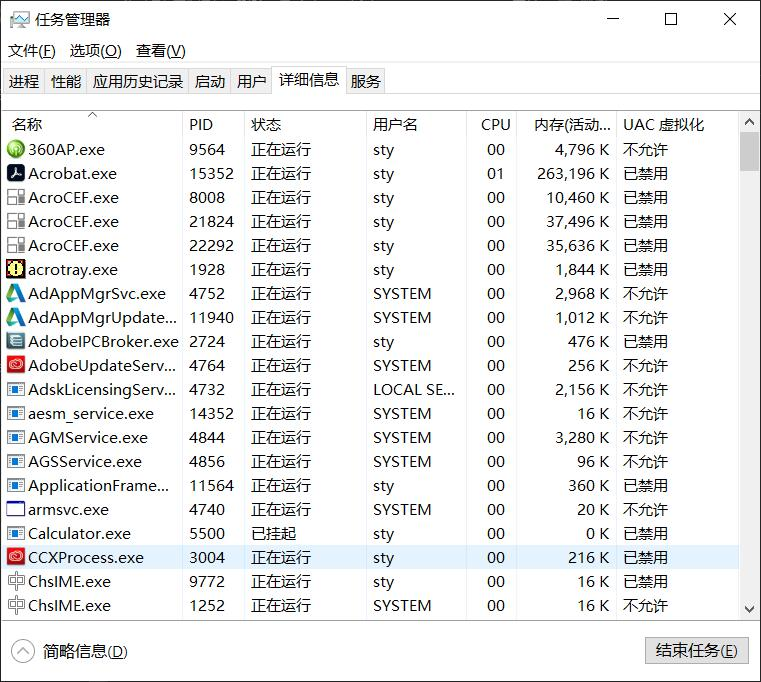
\includegraphics[width=0.7\linewidth]{screenshot001.jpg}
	\caption{进程运行状态信息}
	\label{fig:renwu}
\end{figure}
右边第一列是程序名,第二列PID列出的就是当前所有已运行程序的进程号,没有看到 命令行窗口程序(cmd)进程。

(2)	产生两个命令行窗口新进程。创建过程如图所示。

①打开两个命令行窗口。连续两次执行命令行窗口程序。
②査看命令行窗口程序的进程信息。切换到任务管理器窗口。
可以看到任务管理器窗口中新增了两行命令行程序"cmd.exe"进程信息,其进程号分别为5600和7084。

(3) 通过应用程序界面关闭进程。

1.关闭一个命令行窗口程序。
点击窗口关闭标签。

2.査看命令行窗口程序的进程信息切换到任务管理器。
可以看到进程号为5600的命令行窗口进程消失。

(4)	通过任务管理器关闭进程。
右击7084号进程-"结束进程",余下命令行窗口将被关闭,回到了原先的状态。

\subsection{实验小结}
这是一个很简单的实验,我理解了端与进程关系,了解了进程的基本概念,了解了进程的基本运行原理,掌握了基本进程管理技能。实验没有遇到困难。并且我还通过netstat -ano看到了每个进程所占用的端口号。


\section{网络端地址实验}
\subsection{实验目的}
网络端地址用于标识计算机网络进程,网络进程是计算机网络传输主体,由于语言表达上问题,容易误将计算机作为计算机网络的传输主体。明确了网络传输主体,就容易理解计算机网络各项具体功能处理的基本原理。本实验利用浏览器上网这个最为熟悉的应用,呈现网络 端地址作用。
(1)	明确计算机网络交互的主体是进程。计算机网络两台计算机之间的交互,实质上是两个进程之间的交互。
(2)	了解网络端地址构成及使用。端地址是用于标识网络上任意一台计算机上的任意一个网络进程,具有唯一性和不变性,只有通过访问网络端地址才能通过网络同该进程交互。但在日常使用应用协议时,常常忽略端口地址,自动釆用该应用协议缺省端口地址作为网络端地址。 
\subsection{实验设备}
实验环境由一台计算机来担当实验设备,计算机必须连接互联网。使用浏览器访问互联网任意一个网站,其目标网站的端地址为"www.XXX.com:80", "XXX"代表任意域名。
\subsection{实验网络拓扑}
网络端地址实验拓扑结构如图\ref{screenshot001}所示。
% TODO: \usepackage{graphicx} required
\begin{figure}[htbp]
	\centering
	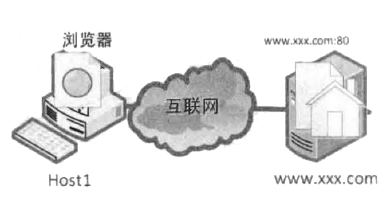
\includegraphics[width=0.7\linewidth]{image/screenshot001}
	\caption{网络端地址实验拓扑结构}
	\label{fig:screenshot001}
\end{figure}
\subsection{实验内容}
启动浏览器,通过访问同一个网址的不同端口,实验中使用了同济大学官网,实际可以是任何一个网址。

(1)	访问非80端口。地址栏中输入http://www.tongji.edu.cn:81,访问如图\ref{fig:screenshot003}所示。
% TODO: \usepackage{graphicx} required
\begin{figure}[htbp]
	\centering
	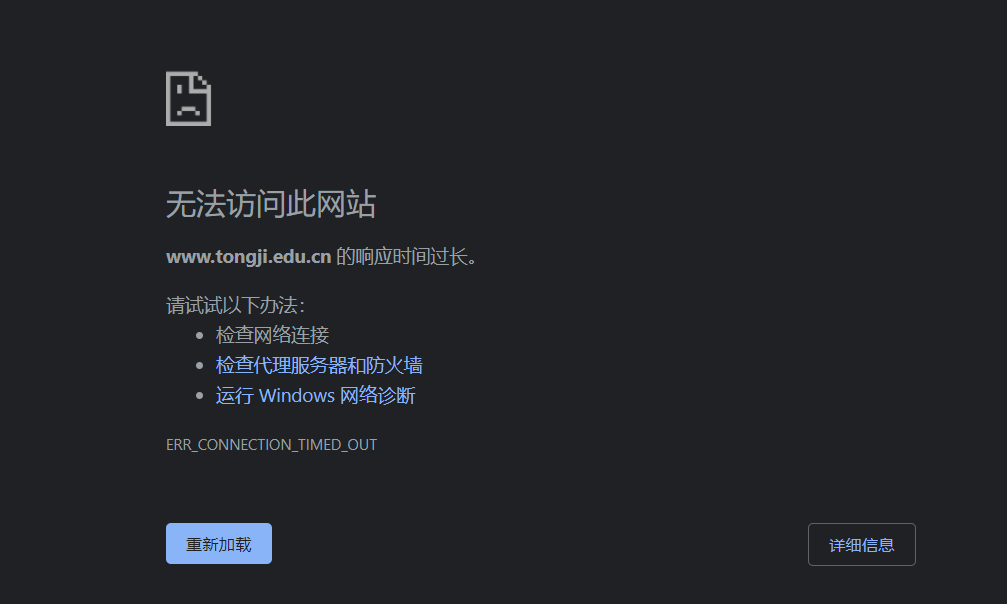
\includegraphics[width=0.7\linewidth]{image/screenshot003}
	\caption{无法访问网站}
	\label{fig:screenshot003}
\end{figure}

浏览器显示无法获得该URL地址网页,Web服务器端口地址不是81.

(2)	访问80端口,地址栏中输入"http://www.tongji.edu.cn:80",如图\ref{fig:screenshot002}所示。浏览器能正常显示网站主页内容。
% TODO: \usepackage{graphicx} required
\begin{figure}[htbp]
	\centering
	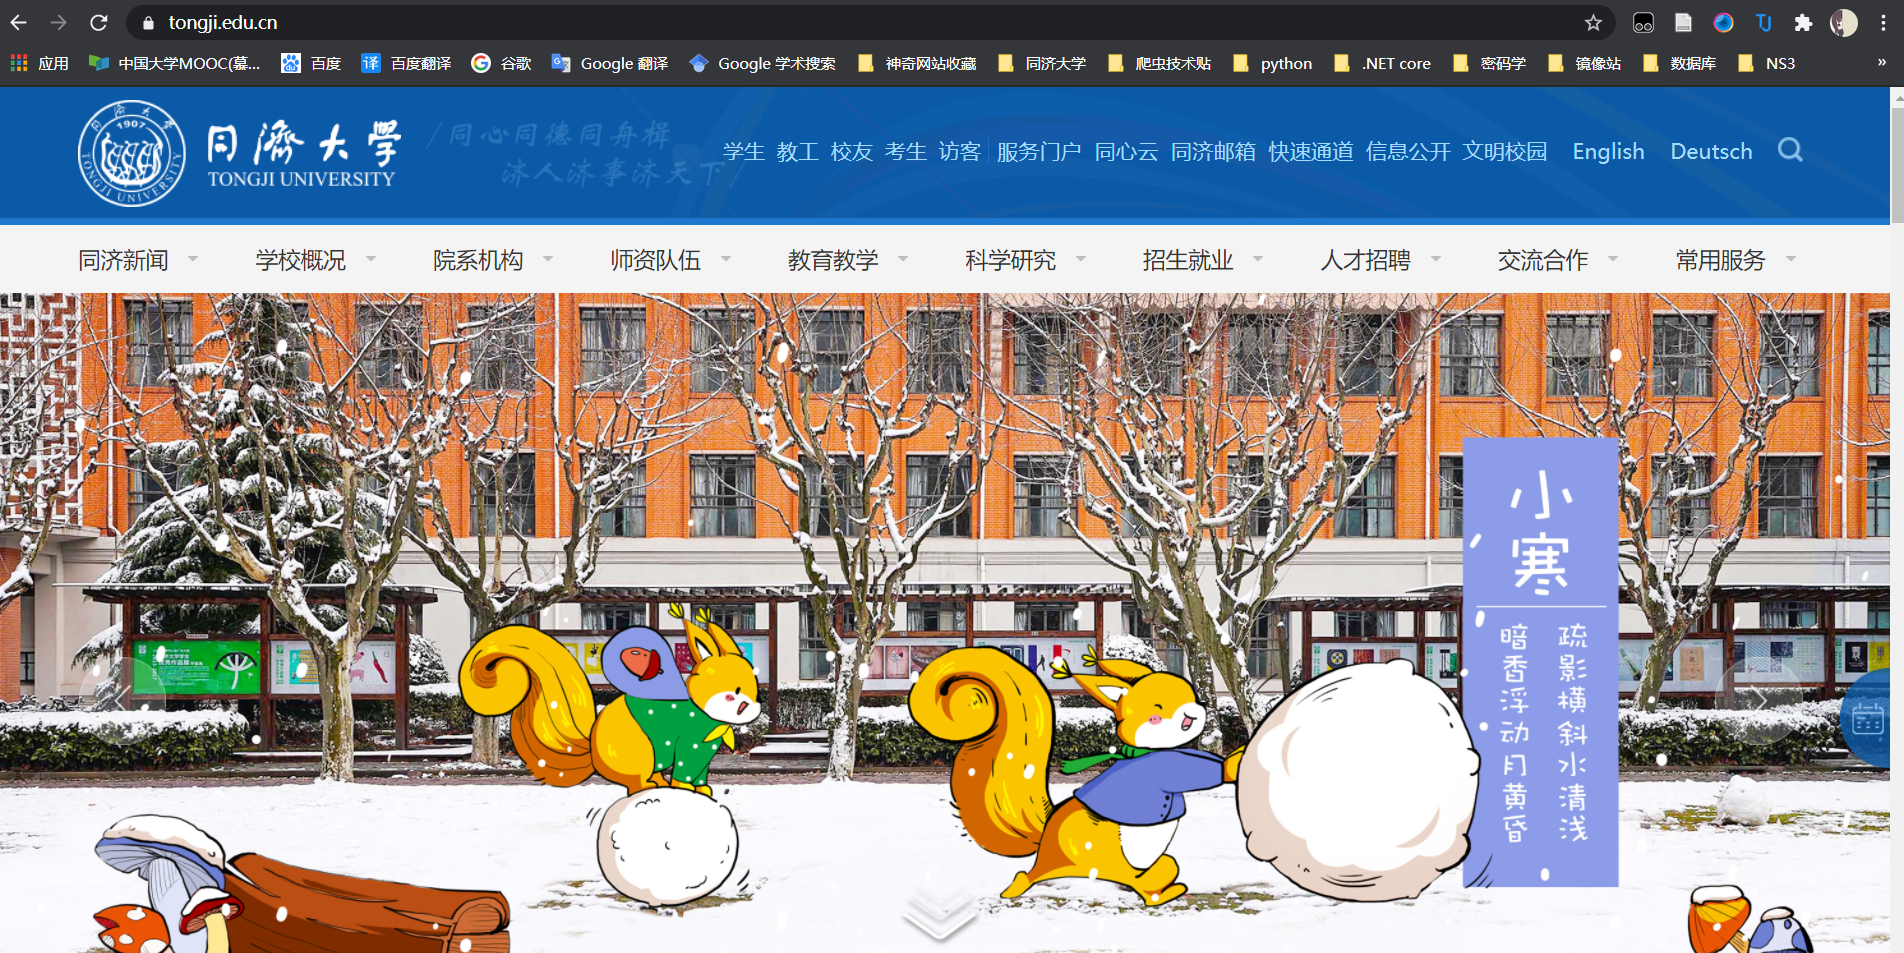
\includegraphics[width=0.7\linewidth]{image/screenshot002}
	\caption{正常访问网页}
	\label{fig:screenshot002}
\end{figure}

\subsection{实验小结}

网络端地址实验也是非常简单的实验,没有遇到任何问题。我们访问服务器的特定服务都需要指定一个特殊的端口,比如smtp协议的25端口,pop3协议的110端口,数据库使用的3306端口,https使用的443端口等等。
\section{网络线的制作和测试实验}
\subsection{实验目的}
了解以太网网络线的制作方法,深入理解物理网络的传输方式。
\subsection{实验设备}
两个TJ45水晶头,一段五类双绞线。
压线钳和网络电缆测试仪。

\subsection{实验内容}
制作一个插头,其步骤:

	1.用压线钳将网线一端的套管皮剪掉2cm。

	2.按照白橙、橙、白绿、蓝、白蓝、绿、白棕、棕线序把网线排列好。

	3.把网线摆平拉直,剪齐留下1.5cm。

	4.将水晶头有塑料弹簧片的一面向下,有金属针脚的一面向上,将线插入水晶头,并使其紧紧地顶在顶端。

	5.把水晶头插入压线钳套住水晶头用力压,使得网线和水晶头卡在一起。 

同样方法制作另一个插头

使用以太网测试工具,将网线线两端头插入网线测试仪,灯亮表示测试通过。 
\subsection{实验小结}

本次实验室我在计算机网络实验中遇到的第一个有一定难度的实验,比较考验我们的动手能力,如果没有掌握技巧,很可能在第五步"把水晶头插入压线钳套住水晶头用力压,使得网线和水晶头卡在一起"这一步失败。不过在多次尝试后,终能领略到"做网线原来如此简单"。
\section{ISO基本操作实验}
\subsection{实验目的}
1.理解实验网络物理组网原理

2.登录路由器

3.熟悉路由器操作系统ISO基本操作

\subsection{实验设备}
两台路由器,一台交换机,两台主机。

\subsection{实验网络拓扑}

% TODO: \usepackage{graphicx} required
\begin{figure}[htbp]
	\centering
	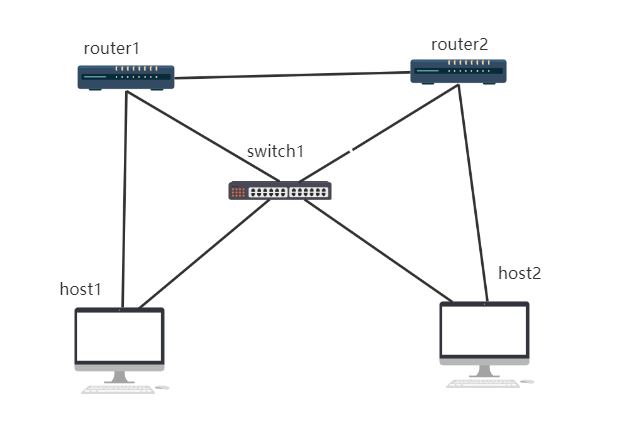
\includegraphics[width=0.7\linewidth]{image/screenshot004}
	\caption{实验网络拓扑}
	\label{fig:screenshot004}
\end{figure}

\subsection{实验内容}
\subsubsection{实验内容1}
1.观看物理连接,理解网络拓扑

2.登录路由器

--打开计算机电源

--选择系统1

--关闭防火墙

--建立HyperTerminal:开始$\rightarrow$程序$\rightarrow$附件$\rightarrow$通讯$\rightarrow$超级终端$\rightarrow$名称=router$\rightarrow$连接=com1$\rightarrow$Baut Rate=9600,8,no parity, 1 stop bit$\rightarrow$呼叫

--断开:HyperTerminal$\rightarrow$断开
\begin{table}[htbp]
	\centering
\begin{tabular}{|l|l|l|l|l|}
	\hline Command Mode & Access Method & Password & Prompt Displayed & Exit Method \\
	\hline User Exec 用户 & Log in & Virtual & $>$ & Logout \\
	\hline Privileges Exec & enable & Enable Secret & $\#$ & disable \\
	\hline Global Configuration 配早 & Config t & & (config)$\#$ & Exit/ctrl+Z \\
	\hline Interface Configuration 端口配早 & Inter & & (config-if)$\#$ & Exit/ctrl+Z \\
	\hline
\end{tabular}
\caption{ISO路由器模式}
\end{table}
\subsubsection{实验内容2}
\begin{lstlisting}
ISO基本命令
1 ?
操作帮助
--寻求帮助:router01> ?
--寻求帮助:router01> sh ?
2 show
--寻求帮助:router01> sh ?
--查看系统配置:router01> sh version
--查看路由表:router01>sh ip route
--寻求帮助:router01> sh ?
--寻求帮助:router01> sh in ?
--寻求帮助:router01> sh int g ?
--查看以太网口配置:router01> sh int gt 0/0
--寻求帮助:router01> sh int ser ?
--查看串口配置:router01> sh int serial 0/0
--查看路由表配置信息:router01> sh running-config  #权限不够
3 enable
--进入特权模式:router01>en(able) ,Enable Secret Password=cisco
--查看路由表配置信息:router01# sh running-config 
--寻求帮助:router01# sh int g ?
--查看以太网口配置:router01# sh in g 0/0
--寻求帮助:router01# sh int ser ?
--查看串口配置:router01# sh int serial 0/0
4 config
--进入配置模式:router01#config t
--寻求帮助:router01(config)# ?
5 interface
--寻求帮助:router01# inter fast ?
--进入以太口:router01(config)#int g 0/0
--修改IP地址: router01(config-if)#ip address 192.168.x.2
6 end
--退到特权模式:router01(config-if)#end(ctrl+z), exit
--查看以太网口配置:router01# sh int g 0/0
7 ping 
--连通测试命令: router01# ping 192.168.x.254
8 shut
关闭端口
--进入配置模式:router01#config t
--进入以太口:router01(config)#int g 0/0
--关闭端口功能:router01(config-if)#no shut
--退到特权模式:router01(config-if)#end(ctrl+z), exit
--查看以太网口配置:router01# sh int g 0/0
9 no
反命令
--进入配置模式:router01#config t
--进入以太口:router01(config)#int g 0/0
--打开端口功能:router01(config-if)#no shut
--退到特权模式:router01(config-if)#end(ctrl+z), exit
--查看以太网口配置:router01# sh int gt 0/0
--进入以太口:router01(config)#int g 0/0
--删除IP地址: router01(config-if)#no ip address <ipaddress><subnet mask>

\end{lstlisting}
\subsection{实验小结}
本次实验是ISO路由器基本操作试验,是后面所有实验的基础,因为后面的每次实验都需要通过命令行来操作路由器和交换机。实验内容非常简单,只需要跟着教程做就可以做出来了,本次实验了解了很多ISO操作系统的常用命令,为后面的实验打好了基础。

这段在第一次在服务器上看到的实验清单里有所以我就写了,后来又重发了个实验清单,里面没出现这个实验,因为已经写了所以就没删。

\section{UDP协议网络编程实验}
\subsection{实验目的}
UDP协议应用面没有TCP协议广,但影响也很大,如微信和QQ等都是典型的UDP应用。UDP网络编程原理基本相同。本实验是使用Socket来编写一个基于UDP简易通信程序,进行即时通信。

(1)	理解客户机/服务器模型,了解端口在网络传输中的作用。

(2)	了解无连接通信方式及编程方式。

(3)	了解掌握基于Socket的UDP应用编程的基本步骤。 

\subsection{实验设备}
一台安装了java的电脑,老师使用的IDE是Eclipse,我使用的是IDEA.
\subsection{实验内容}
运行Eclipse开发平台,并选择已创建Socket项目。

(1)	创建Java包"edu.tongji.networklab.udp"

右击项目 "MSocket/Java Resources/srcw"

"New"->"Package"

输入包名"Name=edu.tongji.networklab.udp"->"Finish"。创建该包用于存放 UDP 实验类。

(2)	开发UdpClient类。

	1.创建 UdpClient类。在包"edu.tongji.networklab.udp"下,创建 UDPClient类。 

右击"src/edu.tongji.networklab.udp"->"New"->"Class".

Name=UdpClient,选择"public static void main(String[ ] arg) "—>"Finish".

	2.输入实验代码。用附录2中UdpCIient源代码完全覆盖初始代码

	3.保存。保存包含着对Java编译,键入"Ctrl+S"或菜单"File"—>"Save"。

(3)	开发UdpServer类

	1.创建 UdpServer 类;类似 UdpCIient,在"edu.tongji.networklab.udp"下,创建 UDPServer类。 

右击"src/edu.tongji.networklab.udp"->"New"->"Class"->"Name=UdpServer",选择"public static void main(String[ ] args)"—>"Finish"

	2.代码开发。输入实验源代码,用附录2中UdpServer源代码完全覆盖初始代码。

	3.保存。保存包含着对Java编译,键入"Ctrl + S"或菜单"File"->"Save"。

(4)代码运行测试。

	1.运行UdpServerC

右击UdpServer—"Run as"->"Java Application"。

	2.运行 UdpClient 发送。同上,右击"UdpClient"->"Run as"->"Java Application"。

点击"连接",然后在发送区输入"hello"->"发送"。

	3.接收文本。
UdpClient的接收区显示"hello";左下角是UdpServer控制台,显示UdpServer收到的客户端请求数据"hello",实验成功。

下面是本次实验的截图。

% TODO: \usepackage{graphicx} required
\begin{figure}[htbp]
	\centering
	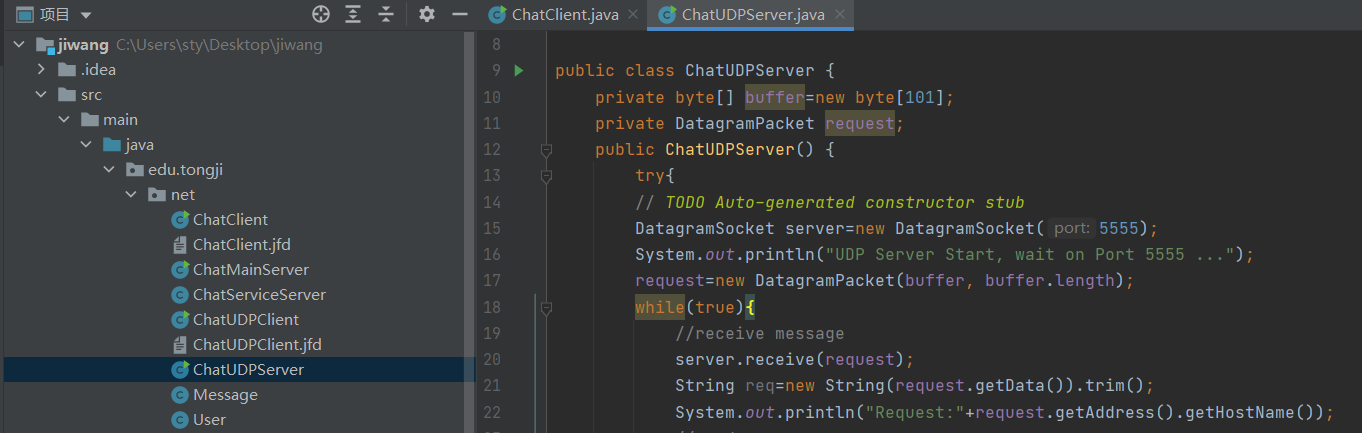
\includegraphics[width=0.9\linewidth]{image/screenshot006}
	\caption{部分代码截图}
	\label{fig:screenshot006}
\end{figure}


% TODO: \usepackage{graphicx} required
\begin{figure}[htbp]
	\centering
	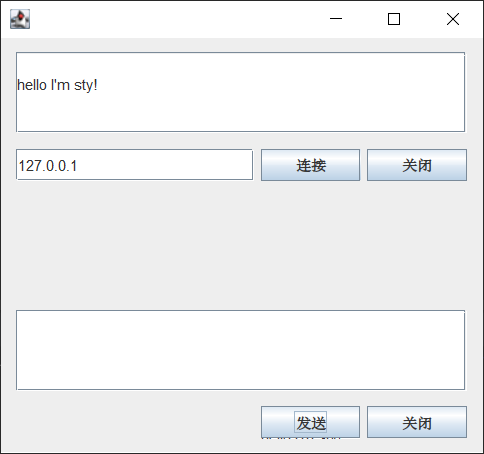
\includegraphics[width=0.7\linewidth]{image/screenshot005}
	\caption{实验截图}
	\label{fig:screenshot005}
\end{figure}


\subsection{实验小结}
实验代码金老师已经帮我们写好了,所以我们很快做完了实验,但是关键是要领会试验运行的原理,而不是只关注实验运行的结果。

这段也是在第一次在服务器上看到的实验清单里有所以我就写了,后来又重发了个实验清单,里面没出现这个实验,因为已经写了所以就也没删。

\section{TCP应用协议编程实验}
\subsection{实验目的}
TCP是使用最为广泛的传输层协议,绝大多数的网络应用服务器都使用TCP协议以保证数据传输可靠,但工程上服务器还需要具有并发能力,允许多个客户并发访问。本实验是使用Socket来编写一个基于TCP简易通信程序,且具有并发能力。
(1)	了解基于TCP网络应用服务器的基本编程架构。
(2)	了解面向连接和无连接的区别,了解TCP编程基本步骤。
(3)	了解并发服务原理及编程方式。

\subsection{实验设备}
一台安装了java的电脑,老师使用的IDE是Eclipse,我使用的是IDEA.

\subsection{实验内容}
创建实验项目目录的过程和上一个实验相似,这里不再赘述。关键点如下:

在Java项目Socket下,开发服务器程序和客户机程序。

(1)	开发服务器程序,创建并实现MainServer类和ServiceServer类,将附录3的MainServer类和ServiceServer类全部源代码复制进去。

(2)	开发客户机程序TCPClient类,为方便实验,TCPClient包含图形化界面,代码较长,将附录3的TCPClient全部源代码复制进去。

(3)	测试交互。先运行MainServer,后运行TCPClient,将连续创建两个TCPClient进程,并同时访问服务器,然后在TCPClient界面中输入字符串,测试并发通信服务。

下面是本次实验我的截图,如图\ref{fig:screenshot008} 图\ref{fig:screenshot007}:

% TODO: \usepackage{graphicx} required
\begin{figure}[htbp]
	\centering
	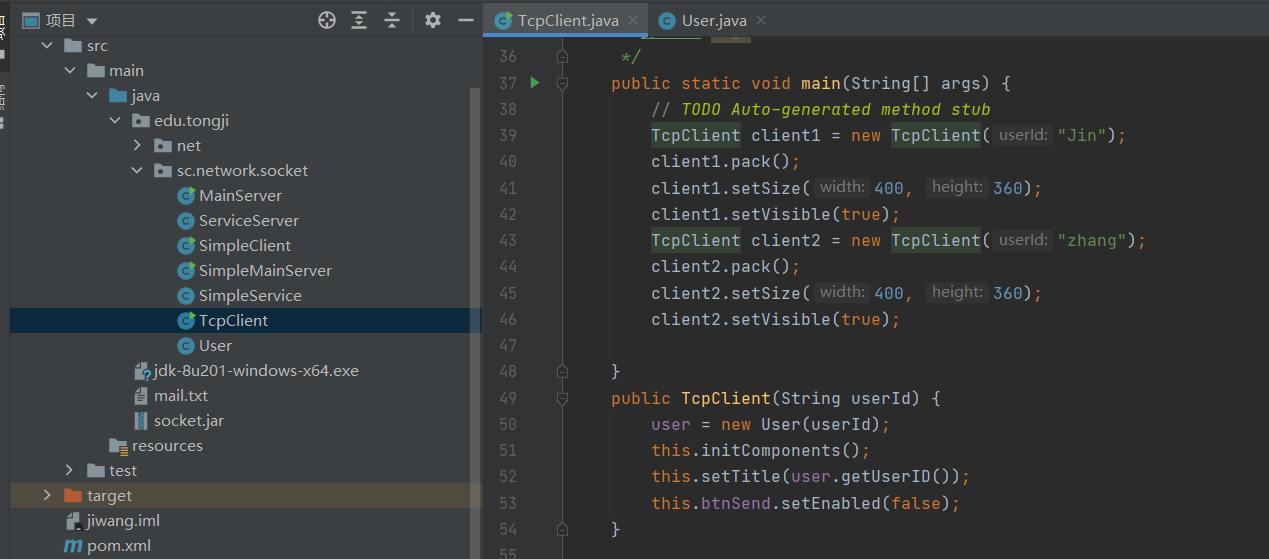
\includegraphics[width=0.8\linewidth]{image/screenshot008}
	\caption{部分代码截图}
	\label{fig:screenshot008}
\end{figure}



\begin{figure}[htbp]
	\centering
	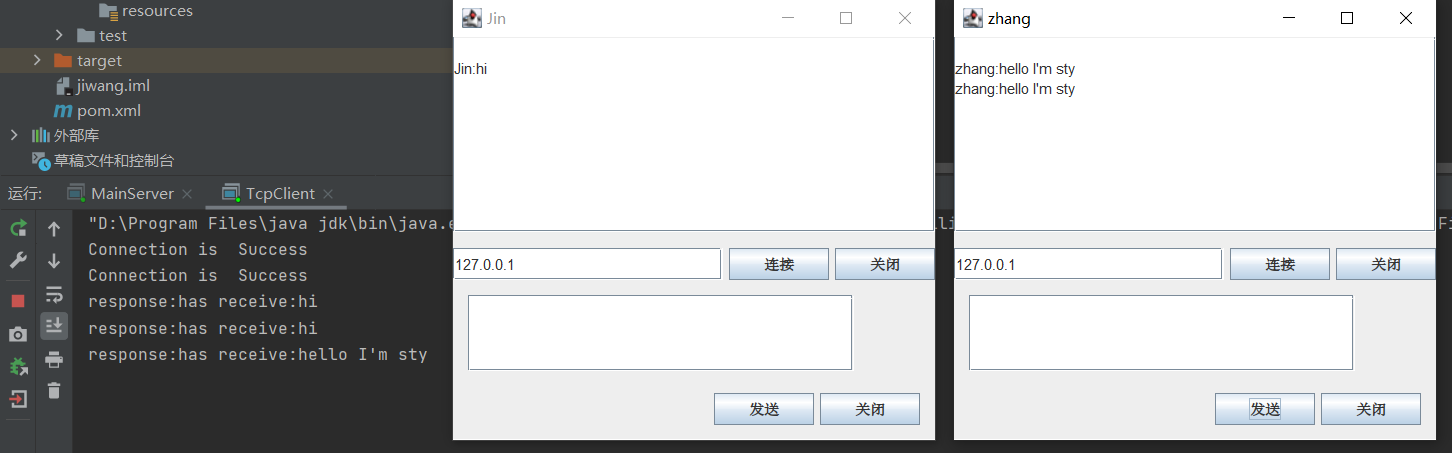
\includegraphics[width=0.8\linewidth]{image/screenshot007}
	\caption{实验截图}
	\label{fig:screenshot007}
\end{figure}


\subsection{实验小结}
这个实验和上个实验很像,TCP和UDP都是传输层协议,但具体的细节有很多很多的不同。实验代码金老师已经帮我们写好了,所以我们很快做完了实验,但是关键是要领会试验运行的原理,而不是只关注实验运行的结果。
\section{端口扫描实验}
\subsection{实验目的}
端口扫描是应对主机入侵而釆取的基本防范措施,掌握端口管理的基本技能是应对网络攻击的必备技能。本实验将使用开源的专业端口扫描软件工具nmap,对子网内的主机进行端口扫描。
(1)	了解端口开放含义。
(2)	了解安全漏洞含义。
(3)	了解掌握网络漏洞扫描工具的使用。
(4)	使用服务管理对端口进行管理。

\subsection{实验设备}

主机需要安装nmap软件。两台计算机和一台交换机担当实验设备,使用两根以太网络线,将两台计算机网卡和交换机连接起来,构成一个子网。主机Hostl作为端口扫描操作平台,另一台主机Host2作为扫描的目标平台,可以是任何一种操作系统,目标主机安装 Windows。在操作平台上使用端口扫描工具软件对目标主机进行扫描。实验使用Windows版本nmap作为端口扫描工具软件,nmap是一款开源的软件,需要下载安装。

\subsection{实验网络拓扑}


\begin{figure}[htbp]
	\centering
	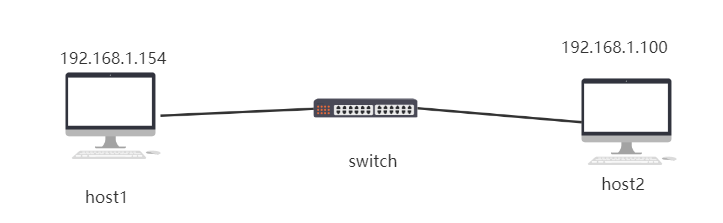
\includegraphics[width=0.7\linewidth]{image/screenshot009}
	\caption{端口扫描网络拓扑}
	\label{fig:screenshot009}
\end{figure}

\subsection{实验内容}

\subsubsection{实验一:远程子网扫描实验}

(1)	配置主机Hostl和Host2地址,主机网卡IP地址设置如下: 

Hostl:IP 地址= 192. 168.1.254,子网掩码=255.255.255.0,网关= 192.168.1.1

Host2:IP 地址= 192. 168. 1.100,子网掩码= 255.255.255.0,网关= 192.168.1.1

(2)	使用nmap扫描软件远程扫描指定子网。对192.168.1.0/24子网进行扫描。

1.Hostl 上启动 nmap。

左击“开始”->“所有程序”->“Nmap”->“Nmap-Zenmap GUI”。

2.扫描192. 168. 1.0/24子网。

输入“目标= 192. 168. 1. * ”,配置=Intense scan->“扫描”,注意扫描要持续一段时间,请保持耐心,在左边会依次列出被扫描的主机IP地址。

3.査看目标主机的端口开放状况。

选择主机192. 168. 1.100,点击“端口/主机”发现了10个开放的端口。

\subsubsection{实验二:端口关闭实验}

如果发现某些端口不用开放,就可以关闭这些端口。实验将关闭目标主机上VM认证服务端口。

(1)进入服务,关闭目标主机上VM认证服务。Host2,右击“开始”->“系统”->“其他管理工具”->“管理工具”->“服务"。

右击 VMware Anthorization Service->“停止”。

(2)重新扫描192.168.1. 100核实。由于nmap是个优秀的软件,所以只要实验网络拓扑没有断开,实验很容易就取得了成功。

实验结果如下图:

\begin{figure}[htbp]
	\centering
	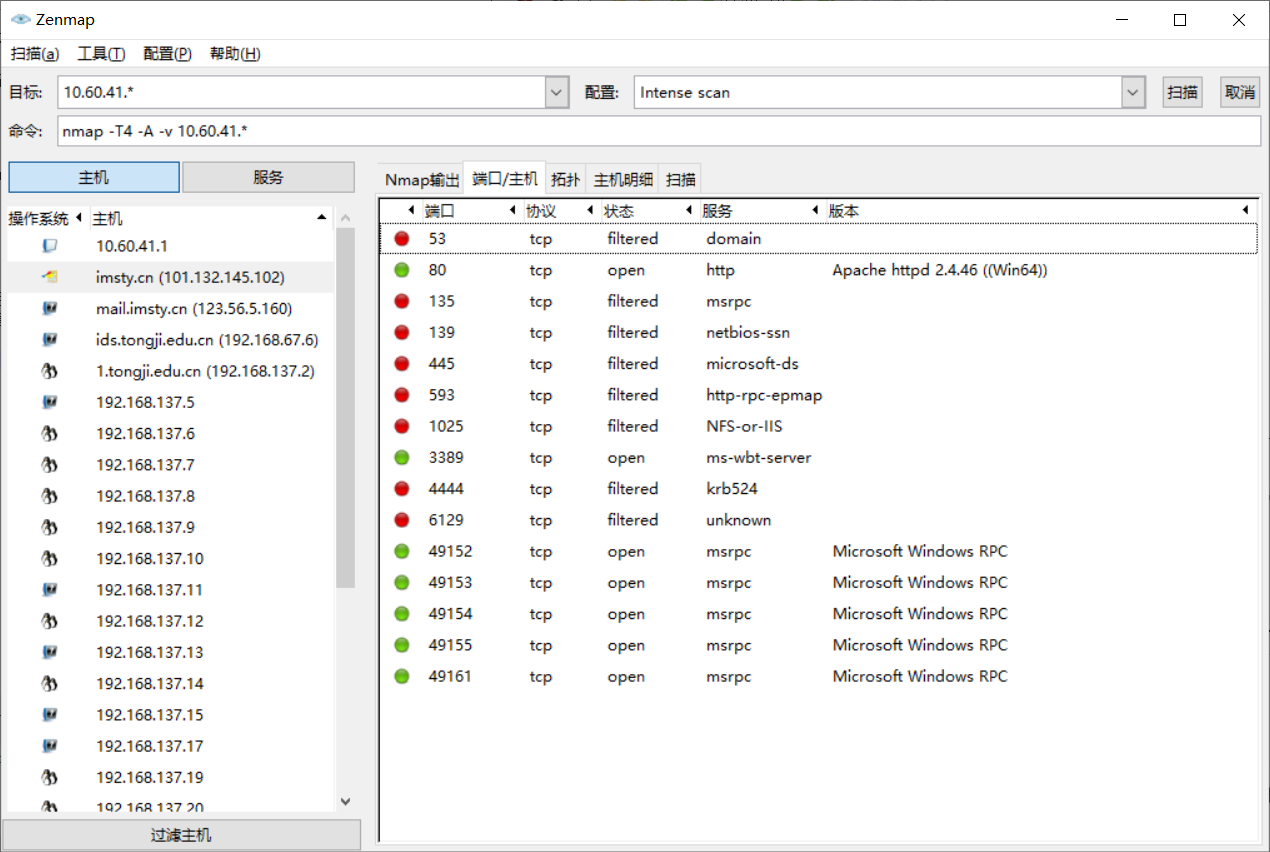
\includegraphics[width=0.7\linewidth]{image/screenshot010}
	\caption{端口扫描}
	\label{fig:screenshot010}
\end{figure}


\subsection{实验小结}
这个实验我记得其实上课金老师没带我们做,因为第一次在服务器上看到的实验清单里有所以我就写了,后来又重发了个实验清单,里面没出现这个实验,因为已经写了所以就没删。实验让我对端口扫描有了一个从感性到理性的认识,开放的网络端口确实比较容易给黑客以可乘之机,这让我想起了臭名昭著的勒索病毒WannaCry,它就是利用了Windows操作系统445端口存在的漏洞。

\section{物理地址解析实验}
\subsection{实验目的}
IP网络不具有实际通信能力,需要将IP数据包封装在物理帧中进行传输,封装前需要对下一跳IP地址进行物理地址解析。物理地址解析是理解IP封装的关键知识点,但物理地址解析行为非常隐蔽,难以察觉。实验利用ARP协议的缓存机制来间接证明物理地址解析行为的发生:
(1)	理解IP网络和物理网络之间的功能关系。
(2)	了解ARP地址解析原理。
(3)	掌握ARPT具软件使用。

\subsection{实验设备}

两台计算机和一台交换机担当实验设备,使用两根以太网络线,将两台计算机网卡都用网 线直接连接交换机。主机Hostl作为地址解析源节点,另一台主机Host2作为地址解析目标节点。使用Windows操作系统自带的ARP工具软件作为实验工具。

\subsection{实验网络拓扑}
\begin{figure}[htbp]
	\centering
	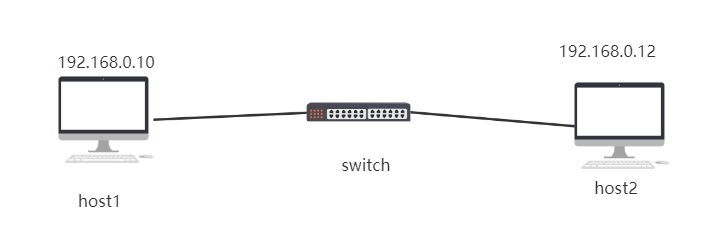
\includegraphics[width=0.7\linewidth]{image/screenshot011}
	\caption{实验网络拓扑}
	\label{fig:screenshot011}
\end{figure}


\subsection{实验内容}

按照实验环境要求,完成实验拓扑结构连接,并打开相关设备电源。

(1)	为Host1和Host2设置IP地址。主机网卡IP地址设置如下:

Host1:IP 地址= 192.168.0.12,子网掩码= 255. 255. 255.0,网关空缺

Host2:IP 地址= 192.168.0.10,子网掩码= 255. 255. 255.0,网关空缺

(2)	Host2触发对Hostl的地址解析。解析如图4-10和图4-11所示。

1.Host2清除ARP缓存表。Host2以管理员身份打开命令行窗口,清除ARP缓存表,以消除有可能存在192. 168. 0.12地址解析条目。

输入:arp-d,清空地址解析缓冲区,以便消除可能已产生的地址解析;

arp -a,显示当前地址解析缓冲区内容,没有出现192. 168.0. 12条目。

2.Host2触发对Host1地址解析,并获得其地址解析缓存。Host2发出ping连通测试命令。

输入“ping 192. 168.0. 12”,测试连通Hostl,触发对192. 168.0. 12的地址解析。

arp-a,显示当前地址解析缓存表内容,岀现了192. 168.0. 12条目,说明在发出连通测试IP数据包前,对192. 168. 0. 12节点的物理地址进行了解析,其解析物理地址是78-36-cc-ee-ab-39。

(3)	核实解析物理地址。Host1打开命令行窗口,核实物理地址。

输入“ipconfig /all”,列出IP地址和物理网卡地址,IP地址是192. 168. 0. 12,物理地址是78-36-cc-ee-ab-39,同Host2解析得到的物理地址完全一致。

实验结果如图\ref{fig:arp} 和图\ref{fig:screenshot012}所示,注意图中红框。

\begin{figure}[htbp]
	\centering
	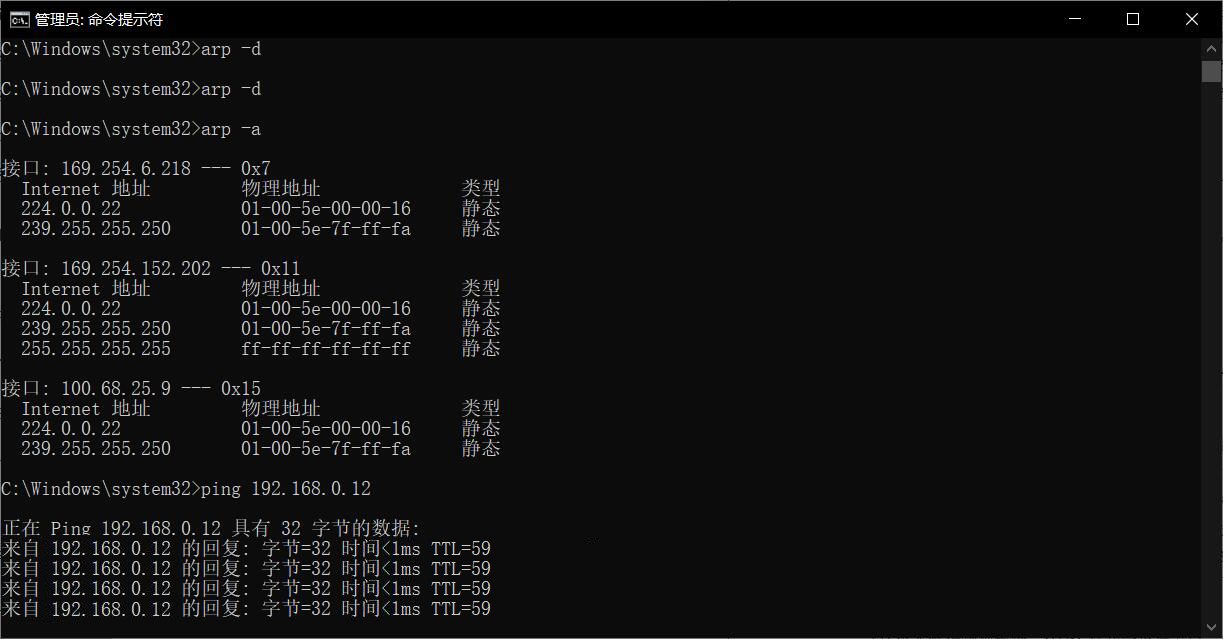
\includegraphics[width=0.7\linewidth]{arp.jpg}
	\caption{物理地址解析实验}
	\label{fig:arp}
\end{figure}


\begin{figure}[htbp]
	\centering
	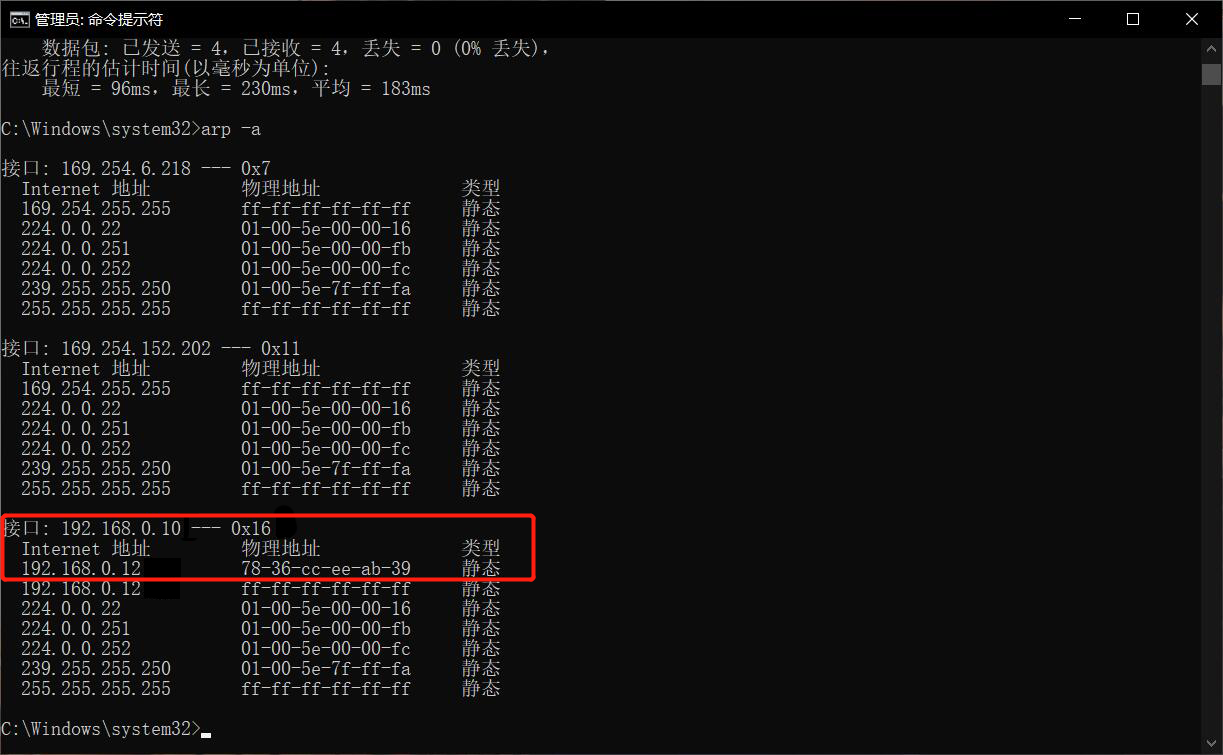
\includegraphics[width=0.7\linewidth]{image/screenshot012}
	\caption{物理地址解析实验图2}
	\label{fig:screenshot012}
\end{figure}


\subsection{实验小结}
物理地址解析实验也是非常重要的实验,实验本身没什么难度,关键在于理解。物理地址解析是通过广播ARP消息来完成的,相当于向局域网里所有主机发出一个问题:“谁拥有IP地址xxx.xxx.xxx.xxx?”然后拥有这个IP地址的主机就会回应。


\section{异步串联通信收发实验}
\subsection{实验目的}
数据通信是物理层的核心功能,其基本原理属于通信学范畴。实验利用计算机的COM口进行两台计算机间的字符收发,展示通信基本原理,加深了解物理层作用。
(1)	理解异步串行通信基本原理。
(2)	熟悉掌握RS-232通信标准以及RS-232帧格式。
(3)	了解波特率等主要通信参数的作用和使用。

\subsection{实验设备}

1. 实验环境主要由两台带COM口的计算机,1根串行交叉线组成;

2. 将单根串行交叉线中间层组成。将单根串行交叉线将两个计算机的COM串口对接起来;

3. 两台计算机超级终端将作为路由器管理的操作平台。

\subsection{实验网络拓扑}

% TODO: \usepackage{graphicx} required
\begin{figure}[htbp]
	\centering
	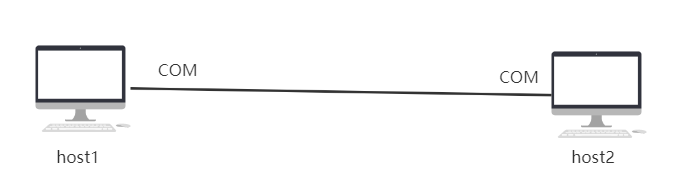
\includegraphics[width=0.7\linewidth]{image/screenshot013}
	\caption{异步串行通信试验网络拓扑}
	\label{fig:screenshot013}
\end{figure}

实验环境主要由两台带COM口的计算机,一根串行交叉线组成。将单根串行交叉线将两个计算机的COM串口对接起来;两台计算机超级终端将作为路由器管理的操作平台。

\subsection{实验内容}

【准备过程】

1. 按照实验拓扑结构要求将两台计算机的COM口用串口反接连接线连接起来。

2. Host1:运行超级终端,建立串口通信连接test1,设置缺省通信参数。

3. Host2:运行超级终端,建立串口通信连接test2,设置缺省通信参数。

\subsubsection{实验1:测试在相同通信参数下的字符传输}

1. Host2的超级终端输入如下内容,此时Host2超级终端无内容显示

\begin{lstlisting}
hello !
\end{lstlisting}

2. Host1的超级终端接收到如下字符串

\begin{lstlisting}
hello !
\end{lstlisting}

\subsubsection{实验2:测试采用不同波特率下的字符传输}

1. Host1和Host2均断开连接,在“文件->属性->配置”中修改参数如下:
\begin{table}[htbp]
	\centering
\begin{tabular}{|c|c|c|c|c|}
	\hline 连接名 & 波特率 & 数据位 & 奇偶校验 & 停止位 \\
	\hline test1 & 4800 & 8 & 奇校验 & 1 \\
	\hline test2 & 9600 & 8 & 奇校验 & 1 \\
	\hline
\end{tabular}
\caption{参数}
\end{table}

2. 进行通信测试。首先在Host1终端从键盘键入以下字符串,Host1屏幕上并不会显示输入内容,
Host2屏幕上显示乱码。

\begin{lstlisting}
7788 test
\end{lstlisting}

3. 在Host2终端从键盘键入以下字符串,Host2屏幕上并不会显示输入内容,Host1屏幕上显示不同乱
码。
\begin{lstlisting}
7788 test
\end{lstlisting}
\subsection{实验小结}

在这个实验中主要是加深我们对物理层网络通信的理性认识。实验1中,两台计算机的通信参数相同,波特率匹配,不会发生帧错误,因此字符传输正常。

而实验2中,两台计算机的波特率不同,则它们单位时间内通信信号发生变化的次数不同,相应的信号采样的频率也不一致,因此两台计算机显示出乱码且乱码值也不相同。

这个实验较简单。通过动手操作串口的字符接收和发送,加深了对通信基本原理的理解。在理解通信基本原理和异步串行传输的基础上,进一步掌握RS-232接口标准以及RS-232帧格式,通过实验1和实验2的具体操作切实理解了通信双方必须要保证波特率匹配才能正确通信,明白了波特率的物理含义。

当然实验中也遇到了一些困难,主要是串口松动接触不良造成的。
\section{主机路由实验}
\subsection{实验目的}

按照网际网组网原理,IP网络是个多跳网络,两个节点之间的传输将穿越多个IP子网,经过多个路由器,才能到达目标主机,而这一切均有赖于路由机制完成。一般认为,路由是路由器的专利。 实际上,主机上也设置了路由表,只是较为隐蔽。主机路由表是理解主机和路由器建立转发关系的 关键所在。实验构建两个IP子网,利用单路由器实现子网互联,验证主机缺省网关作用。

(1)	深入了解主机路由机制。

(2)	了解和掌握主机路由配置方法。

\subsection{实验设备}

实验环境由一台路由器、两台计算机和一台交换机组成。由交换机担当网络连接设备,将路由器两个以太网端口和两台计算机网卡都用网线直接连接到交换机;通过串行线将主机 Host1串口com同路由器Console口连接起来,启用其超级终端作为路由器管理的操作平台。

\subsection{实验网络拓扑}
主机路由实验网络拓扑如图\ref{fig:screenshot014}所示。
\begin{figure}[htbp]
	\centering
	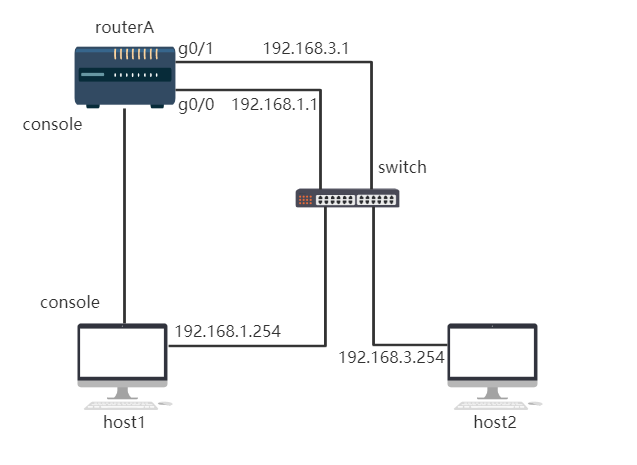
\includegraphics[width=0.7\linewidth]{image/screenshot014}
	\caption{主机路由实验网络拓扑}
	\label{fig:screenshot014}
\end{figure}


\subsection{实验内容}
按照实验环境要求,完成实验拓扑结构连接,并打开相关设备电源。

\subsubsection{实验一:主机路由实验}

(1)	配置主机Host1和Host2地址,并测试子网连通性。

1.配置Host1和Host2地址。主机网卡IP地址设置如下:

Host1: IP 地址= 192. 168. 1. 254,子网掩码= 255. 255. 255. 0,网关=192. 168. 1. 1

Host2:IP 地址= 192. 168. 3. 254,子网掩码= 255. 255. 255.0,网关= 192. 168. 3. 1

2.测试子网连通性。Host1打开命令行窗口。

输入“ping 192. 168. 3. 254”,没有连通,原因是Host1和Host2的网络地址不同,网关地址虽设置了,但网关节点并不存在,设置无法起作用。

3.查看主机Host1主机路由表。Host1使用命令行窗口。

输入"Route print",可以看到缺省路由(0.0.0.0    0.0.0.0)是 192.168. 1. 10

(2)配置RouterA以设置子网网关。启用超级终端,配置路由器两个以太网端口分别成为两个子网的网关。

\begin{lstlisting}
1. 进入配置模式。
进入特权模式:routerA>en, Enable Secret Password = cisco
进入配置模式:routerA# config t
2. 192.168.1.0/24网关配置。
进入g0/0以太网端口配置模式:routerA(config) # int g0/0
设置 IP 地址:router A (config-if) # ip address 192. 168. 1. 1 255. 255. 255. 0
开启端口:routerA( config-if) # no shut
退出端口配置模式,使端口配置生效:routerA(config-if) # exit
3. 192.168.3.0/24网关配置。
进入g0/l以太网端口配置模式:routerA(config) # in g0/l
设置 IP 地址:routerACcon£ig-if) # ip address 192. 168. 3. 1 255. 255. 255. 0
开启端口:routerA( config-if) # no shut
退出端口配置模式,使端口配置生效:routerA(config-if) # exit
4. 启用路由功能。
启用路由功能:routerA(config) # ip routing
退出配置模式,使配置生效:routerACconfig) # exit

\end{lstlisting}

(3)	测试子网连通性。测试主机Host1是否连通主机Host2, Host1中打开命令行窗口,输入"ping 192. 168. 3. 254”,表示Host1已连通主机Host2,主机路由表和主机网关发生作用,发挥了路由器路由转发功能。

\subsubsection{实验二:主机缺省网关实验}

取消主机Host1缺省网关地址,并测试同Host2连通性。

(1)	重置主机Hostl的缺省网关地址。

删除默认网关地址-“确定”。

(2)	测试子网连通性。Hostl打开命令行窗口。

输入“ping 192.168.3.254”,表示不能连通Host2,网关节点存在,但主机的网关地址没有设置,将不能发挥网关节点作用,无法访问其他子网。


\subsection{实验小结}

在实验过程中出现了一些问题,例如接上交换机并配置完每台主机的IP和子网掩码后,利用ping进行连通性测试失败,后经检查后发现网线刚接上交换机时交换机对应端口的灯为红色,等待灯变成绿色后可以成功ping通,猜测是因为此段时间交换机在获取主机的IP地址或者MAC地址。

在实验时,用网线将路由器的FE 0/1口和FE 0/0口和交换机相连,路由器和交换机对应端口的灯亮,但是过一会之后路由器上的FE 0/1端口灯灭了,对应的交换机端口上的灯也灭了,我以为是路由器坏了,后来发现,在对路由器进行操作,输入no shut命令开启FE 0/1端口之后灯又亮了,由此我明白了为什么开启端口的命令叫做no shut。在对路由器进行操作的时候碰到的另一个问题是,我根据书上的命令进行输入,输入int g0/0回车,命令行报错,经过排查之后发现我使用的路由器上的端口名称不是g0/0而是 FE 0/0,这可能是因为路由器不是千兆路由器而是百兆路由器,因此我将命令改成了int f0/0,遂成功。

在实验中还遇到了另外的问题是,所有操作均正确,但是主机却ping不通,根据老师的点拨,是因为交换机可能已经划分了多个VLAN,因此更换接线的端口之后成功ping通。
\section{以太网组网实验}
\subsection{实验目的}

物理网络是计算机网络的基本组织单元,其各个节点之间可以进行数据通信。物理网络是互联网的基础架构,无论对于理解网络基本原理还是网际互联原理都非常关键。实验利用以太网交换机组成一个独立的双绞线以太网物理网络,实现网络节点之间的互通。

(1)	理解局域网组网原理。

(2)	理解掌握以太网组网步骤。

(3)	了解以太网网络地址格式。

\subsection{实验设备}

两台计算机和一台交换机担当实验设备,使用两根双绞线网线,将两台计算机以太网网卡同交换机连接起来。计算机Host1作为操作平台和测试操作平台,另一台计算机Host2作为测试平台。也可以使用家用无线路由器代替交换机,开展本实验。

\subsection{实验网络拓扑}

如图\ref{fig:screenshot015}所示

\begin{figure}[htbp]
	\centering
	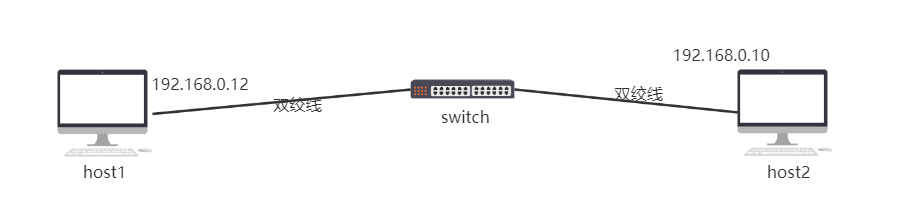
\includegraphics[width=0.7\linewidth]{image/screenshot015}
	\caption{组网实验实验网络拓扑图}
	\label{fig:screenshot015}
\end{figure}

\subsection{实验内容}

\subsubsection{实验一:以太网组网试验}

(1)	用两根双绞线网线分别将两台计算机网卡同交换机端口连接起来,这样就形成了局域网。

(2)	为主机配置IP地址。限于篇幅,请参考1.4. 1小节,主机网卡IP地址设置如下。

Hostl:IP 地址= 192. 168. 0. 12,子网掩码= 255. 255. 255.0

Host2:IP 地址= 192. 168. 0. 10,子网掩码= 255. 255. 255. 0

(3)	Host1测试Host2是否连通。打开Host1命令行窗口。

输入ping命令“ping 192. 168.0. 10”,可以看到连通,由于交换机处理有个延缓过程,命令要多打几次,才能实验成功。

这个地方我印象深刻,交换机上的灯过一会之后会由红变绿,代表可以连通了。

实验截图如下:

% TODO: \usepackage{graphicx} required
\begin{figure}[htbp]
	\centering
	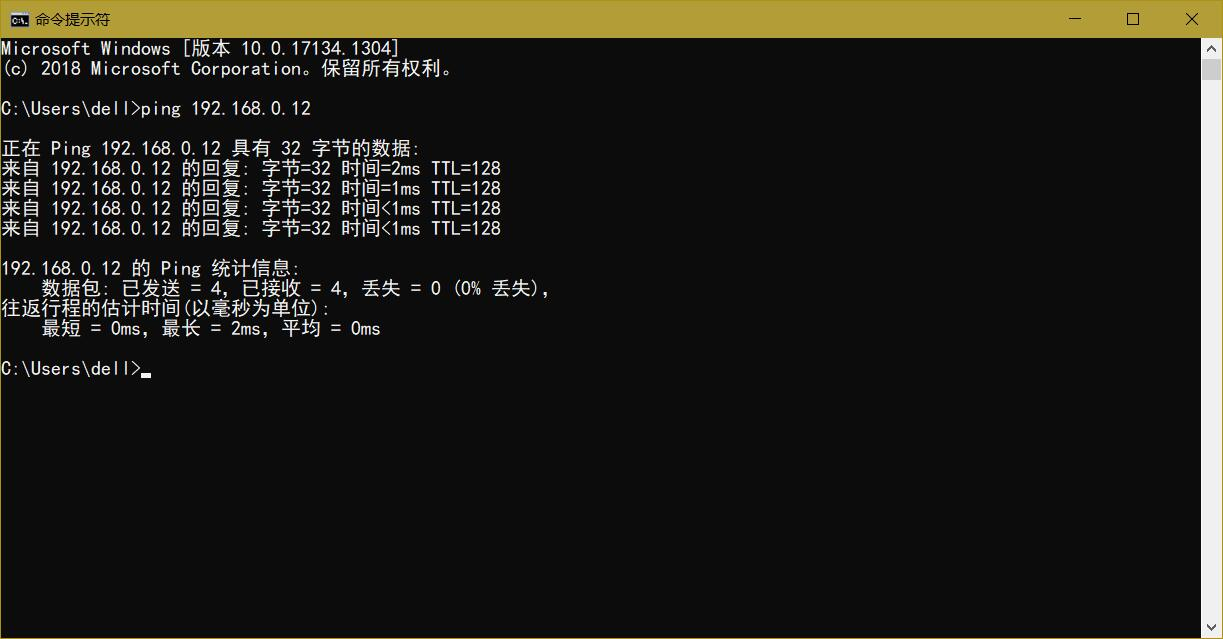
\includegraphics[width=0.7\linewidth]{image/ping}
	\caption{ping通了}
	\label{fig:ping}
\end{figure}



\subsubsection{实验二:以太网卡地址查看实验}

Host1査看自身以太网物理地址,打开命令行窗口。

输入命令ipconfig: ipconfig /all,可以看到Host1以太网卡的IP地址和物理地址。

% TODO: \usepackage{graphicx} required
\begin{figure}[htbp]
	\centering
	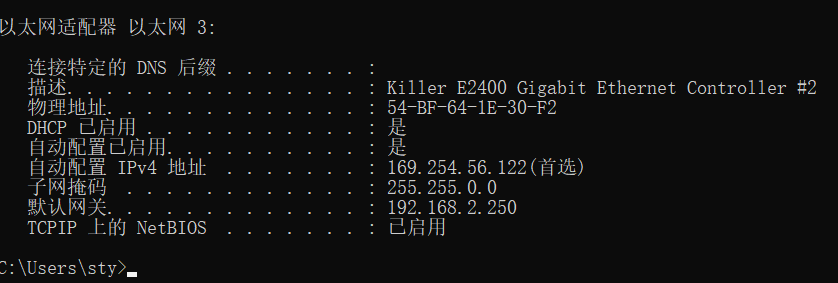
\includegraphics[width=0.7\linewidth]{image/screenshot016}
	\caption{查看地址}
	\label{fig:screenshot016}
\end{figure}


\subsection{实验小结}

这两个实验的内容相当相当的简单,但在当时做实验的时候还是遇到了一点点小问题,例如接上交换机并配置完每台主机的IP和子网掩码后,利用ping进行连通性测试失败,后经检查后发现网线刚接上交换机时交换机对应端口的灯为红色,等待灯变成绿色后可以成功ping通,猜测是因为此段时间交换机在获取主机的IP地址或者MAC地址。

在实验中还遇到了另外的问题是,所有操作均正确,但是主机却ping不通,根据老师的点拨,是因为交换机可能已经划分了多个VLAN,因此更换接线的端口之后成功ping通。

\section{VLAN配置实验}
\subsection{实验目的}

对于企业而言,可能含有许多部门,为便于管理,常常以部门为单位,构建多个物理子网。 传统网络工程,只有相近的办公室才可以组成同一个物理子网,鉴于种种原因,很可能同个部 门的两个办公室位于不同楼层,甚至不同大楼。

虚拟局域网(Virtual Local Area Network, VLAN),标准编号为IEEE 802.IQ,可以实现 将两个相距较远的办公室组成同一个物理子网。实验利用交换机提供虚拟局域网功能,实现VLAN划分。

(1)	了解虚拟局域网基本概念。

(2)	掌握交换机实施虚拟局域网技术。


\subsection{实验设备}

由一台CISCO交换机和两台计算机担当实验设 备,使用两根双绞线网线,将两台计算机以太网网卡同交换机连接起来;通过串行线将计算机Hostl串口 coml同交换机Console 口连接起来,使用超级终端作为交换机的操作平台。


\subsection{实验网络拓扑}

如图,我将不同的端口区分了不同的颜色以区分它们,代表不同的VLAN.

\begin{figure}[htbp]
	\centering
	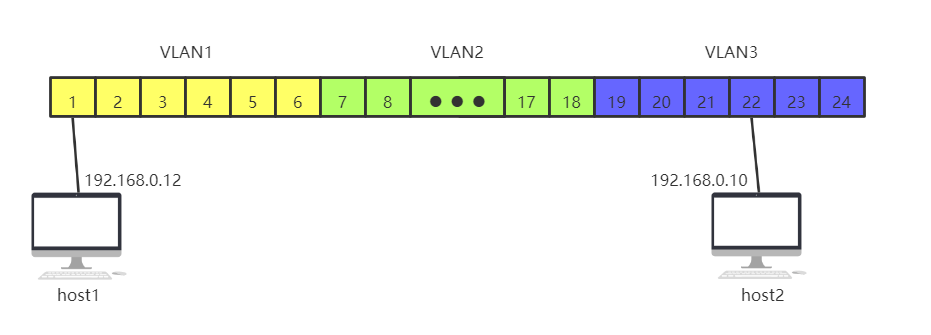
\includegraphics[width=0.7\linewidth]{image/screenshot017}
	\caption{VLAN划分示意图}
	\label{fig:screenshot017}
\end{figure}


\subsection{实验内容}

\begin{lstlisting}
1.未配置前端口通信测试
--配置两主机IP地址:192.168.0.2和192.168.0.5
--连接任意端口
--测试192.168.0.2:ping 192.168.0.5#连通
2配置VLAN2
2.1连接交换机
--使用console线将计算机串口com2与路由器console口直接相连;
--建立HyperTerminal:开始程序附件通讯超级终端名称=switch连接=com2Baut Rate=9600,8,no parity, 1 stop bit;
--进入特权模式:switch01>en(able) ,Enable Secret Password=cisco
2.2 2查看VLAN配置:switch01# sh vlan
2.2.3 建立VLAN2
--进入vlan配置模式:switch01#vlan database
--添加vlan: switch01(vlan)#vlan 2 name vlan2 
--退出:switch01(vlan)#exit
2.2.3 建立VLAN3
--进入vlan配置模式:switch01#vlan database
--添加vlan: switch01(vlan)#vlan 3 name myvlan 
--退出:switch01(vlan)#exit
2.2.4 为VLAN2分配端口
--进入配置模式:switch01#config t
--进入f0/1端口:switch01(config)#in f0/1
--将端口分配给vlan2:switch01(config -if)#switchport access vlan 2
--退出:switch01(config -if)#exit
--查看VLAN2配置:switch01# sh vlan name vlan2
2.2.5.测试
--重新测试192.168.0.2: ping 192.168.0.5 #不连通
2.2.6 为VLAN2分配新端口
--进入f0/24端口:switch01(config)#in f0/24
--将端口分配给vlan2:switch01(config -if)#switchport access vlan 2
--退出:switch01(config -if)#exit
--查看VLAN2配置:switch01# sh vlan name vlan2
2.2.7.测试
--重新测试192.168.0.2: ping 192.168.0.5 #办连通
3配置VLAN3
4 删除VLAN
4.1 删除端口
--进入配置模式:switch01#config t
--进入f0/1端口:switch01(config)#in f0/1
--将端口返回VLAN1:switch01(config -if)#switchport access vlan 1
--将所有端口删除
--退出:switch01(config -if)#exit
4.2 删除VLAN2
--进入vlan配置模式:switch01#vlan database
--添加vlan: switch01(vlan)#no vlan 2
--退出:switch01(vlan)#exit
4.3查看VLAN配置:switch01# sh vlan
4.4 删除VLAN3
--进入vlan配置模式:switch01#vlan database
--添加vlan: switch01(vlan)#no vlan 3
--退出:switch01(vlan)#exit

\end{lstlisting}

实验过程的记录如下,每幅图的含义已经写在每幅图片的下方:


\begin{figure}[htbp]
	\centering
	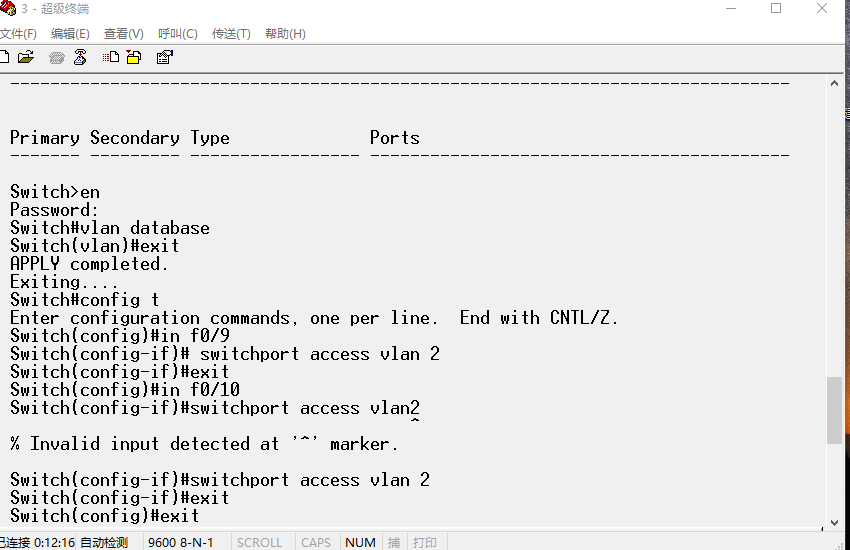
\includegraphics[width=0.7\linewidth]{image/vlan1}
	\caption{为端口指定VLAN}
	\label{fig:vlan1}
\end{figure}

\begin{figure}[htbp]
	\centering
	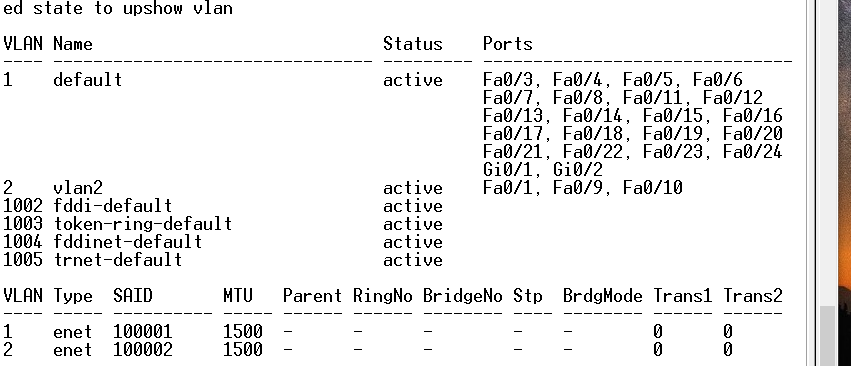
\includegraphics[width=0.7\linewidth]{image/vlan2}
	\caption{查看已经划分的端口}
	\label{fig:vlan2}
\end{figure}

\begin{figure}[htbp]
	\centering
	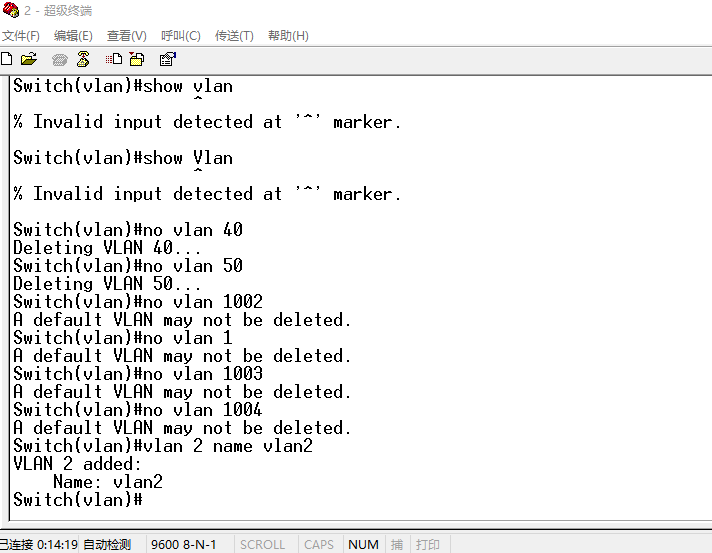
\includegraphics[width=0.7\linewidth]{image/vlan3}
	\caption{删除VLAN以及添加VLAN}
	\label{fig:vlan3}
\end{figure}


\begin{figure}[htbp]
	\centering
	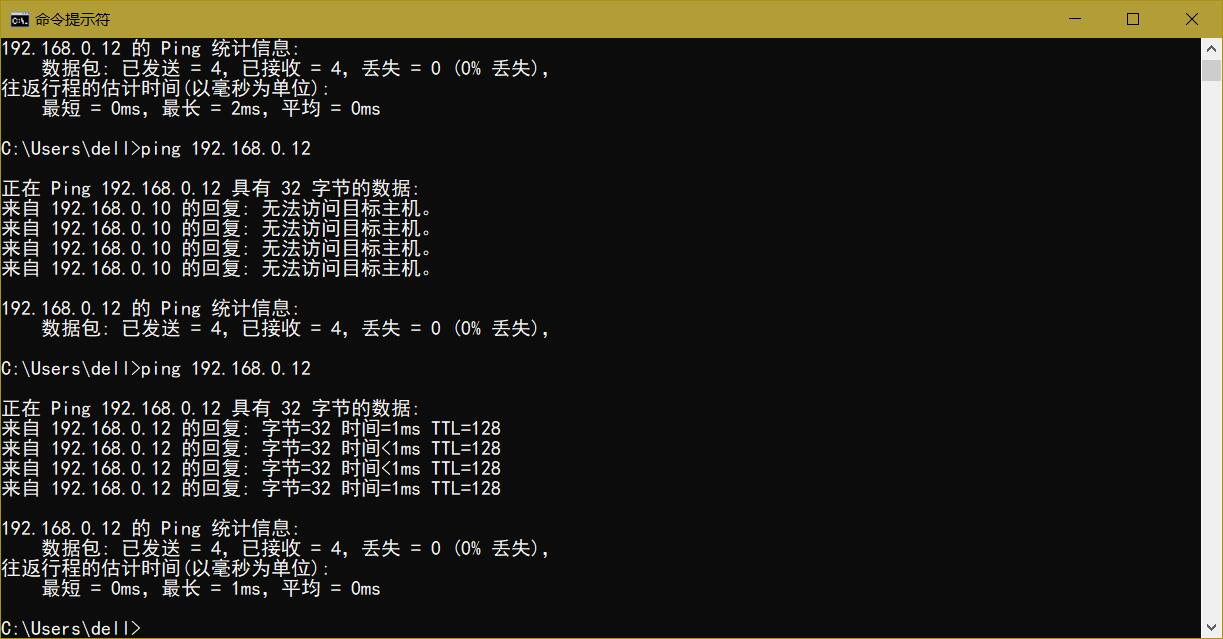
\includegraphics[width=0.7\linewidth]{image/在不同vlan无法访问,在相同vlan可以访问}
	\caption{在不同vlan无法访问,在相同vlan可以访问}
	\label{fig:vlanvlan}
\end{figure}



\subsection{实验小结}

VLAN实验可以算是非常实用的实验了,因为为了局域网的安全,给网络划分不同的区域非常重要。计网实验指定很多,使用也比较复杂,必须静下心来仔细核对,否则就比较容易出错。另外实验室的设备也有时候会出一点问题导致实验进度受到阻碍。

尚未配置VLAN前,VLAN1拥有所有端口,1个VLAN即1个广播域,在同广播域下的192.168.0.10与192.168.0.12可以连通。但如果在不同的VLAN中就无法连通了。

\subsubsection{经验教训}

配置完之后检查一下VLAN分配情况看看是不是你想的那样,而且前面的同学留下来的配置也可能干扰你做实验。

\section{虚拟无线网络实验}
\subsection{实验目的}

无线组网技术是计算机网络组网技术中发展最为迅速的技术,由于无线网络具有的可移动性,发展前景非常广阔,但无线组网技术实验教学却受环境制约因素较大,无论设备数量还是拓扑结构,在现有实验条件下均受到极大限制。

在经过本实验之后,可以对NS3这一平台有更深入的理解。


\subsection{实验设备}
一台安装了VMware的电脑,其中安装Ubuntu 16.04,并配置好NS3的环境。

\subsection{实验内容}

本实验包括两个部分。

\subsubsection{1.无线局域网络隐藏节点实验}

【实验目标】

对无线网络的传输机制有一个直观的了解,加深对CSMA/CA协议的理解。该实验项目中可以随意调整节点的位置,并通过分析实验产生数据结果,来获得最终的实验结论。可以培养初步的观察力和分析能力,形成最基本的研究能力。

【实验原理】

无线局域网络Wireless LANs,简称Wi-Fi,标准版本号是802.11,从此版本又发展了多个子版本,比如熟知的802.11g。但其传输机制是完全一致,所有节点都采用了同频率载波,采用了Carrier Sense On Multi-Access/ Collision Avoid (CSMA/CA),即多路存取载波监听/避免碰撞机制,类似总线的共享发送模式,即任意时刻只有一个节点才能发送。
多路存取载波监听机制,根据监听通道传输状态以决定是否可以发送。

1、当节点需要发送数据时,进行载波监听。载波是网络上的传输信号。

2、如果节点在网络上监听到载波,说明其他节点在发送,那只能耐心等待,返回1。

3、如果没有监听到载波,就能直接往网上发送帧,用不着通知其他节点。这是没有节点在传输数据。

多路存取载波监听机制建立在所有节点都能监听其他任意节点的载波基础上,但在无线网络中,由于其可移动性,会发生隐藏节点问题。

隐藏节点是指在接收节点的覆盖范围内而在发送节点的覆盖范围外的节点。由于听不到发送节点的发送,隐藏节点可能向相同的接收节点发送分组,导致分组在接收节点处冲突。隐藏节点可以分为隐发送节点和隐接收节点。

A和C就互为隐藏节点。节点A和C同时想发送数据给节点B,但A和C都不在对方的传送范围内。所以当A发送数据给B时,C并未检测到A也在发送数据,会认为目前网络中无数据传送,会将数据发送给B。这样,A和C同时将数据发送给B,使得数据在B处产生冲突,最终导致发送的数据不可用。这种因传送距离而发生误判的问题称为隐藏节点问题。

解决隐藏节点的思路是使接收节点周围的邻居节点都能了解到正在进行的传输。RTS/CTS方式是解决隐藏节点问题的主要方法之一,发送节点在数据发送前与接收节点进行一次短控制消息握手交换,请求发送(Request to Send,RTS)和清除发送(Clear to Send,CTS)的控制信息来避免冲突。

发送方发出数据前,先送出一个RTS包,告知在传送范围内的所有节点不要有任何传送操作。如果接收方目前空闲,则响应一个CTS包,告诉发送方可开始发送数据,此CTS包就会告知所有在接收方信号传输范围内的其它节点不要进行任何传输操作。

【实验内容】

隐藏节点实验主要是揭示无线节点传输过程中可能发生的冲突以及解决的过程。实验设置了两个发送节点和一个接收节点,实验中需要控制的是节点之间的距离可以自由调整,RTS/CTS控制可以启用或不启用,然后观察数据包丢失现象来获得实验结论。实验场景如下:

\begin{figure}[htbp]
	\centering
	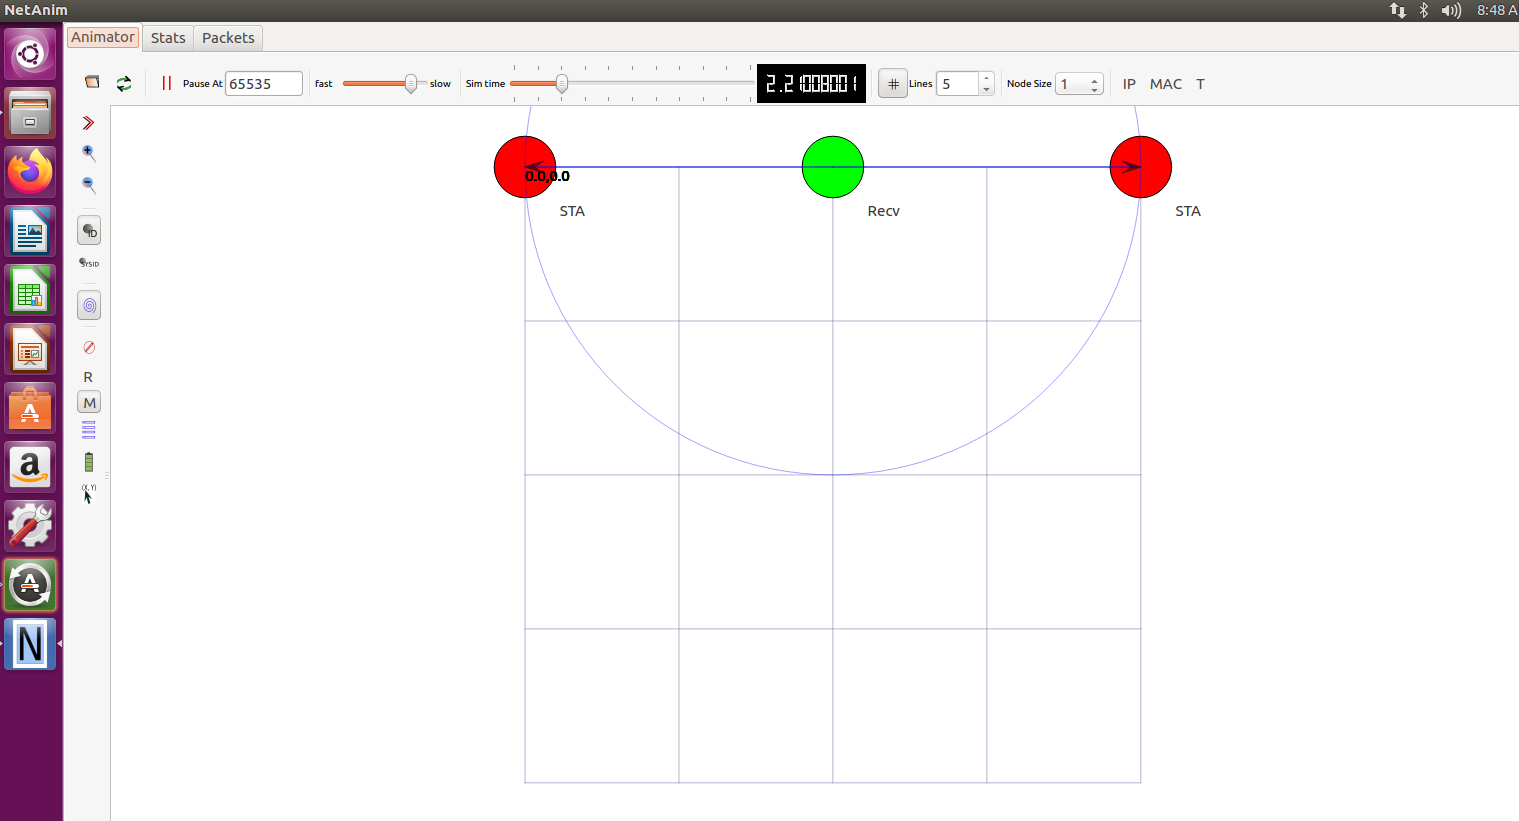
\includegraphics[width=0.7\linewidth]{image/screenshot019}
	\caption{实验场景}
	\label{fig:screenshot019}
\end{figure}

【实验过程】

虚拟实验由wifi-hidden-stations.cc实现。具体步骤:

1、编译wifi-hidden-stations.cc。

1)复制wifi-hidden-stations.cc到NS\_HOME/scratch

2)编译wifi-hidden-stations.cc:./waf –run scratch/wifi-hidden-stations.cc

\begin{figure}[htbp]
	\centering
	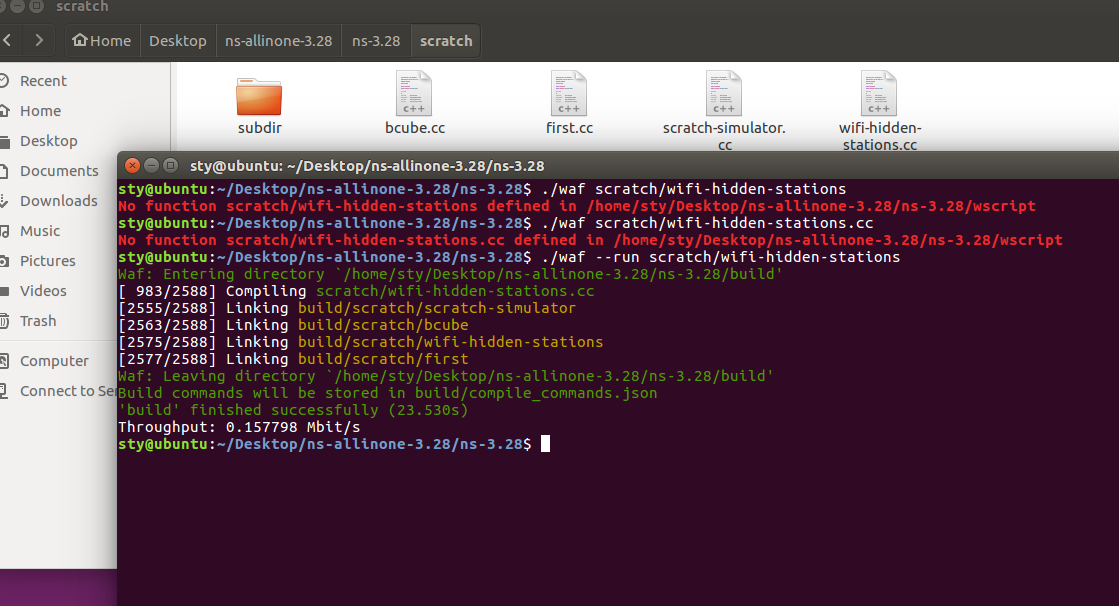
\includegraphics[width=0.9\linewidth]{image/screenshot018}
	\caption{编译并运行wifi-hidden-stations.cc}
	\label{fig:screenshot018}
\end{figure}

2、运行目标代码。

1)将目录移动到NS\_HOME/scratch/build

2)运行目标代码:./ wifi-hidden-stations.cc

3、显示运行动画

1)将目录移动到执行目录netanim

2)启动netanim动画工具程序:./NetAnim

3)显示运行动画。打开wifi-hidden-stations.xml


\begin{figure}[htbp]
	\centering
	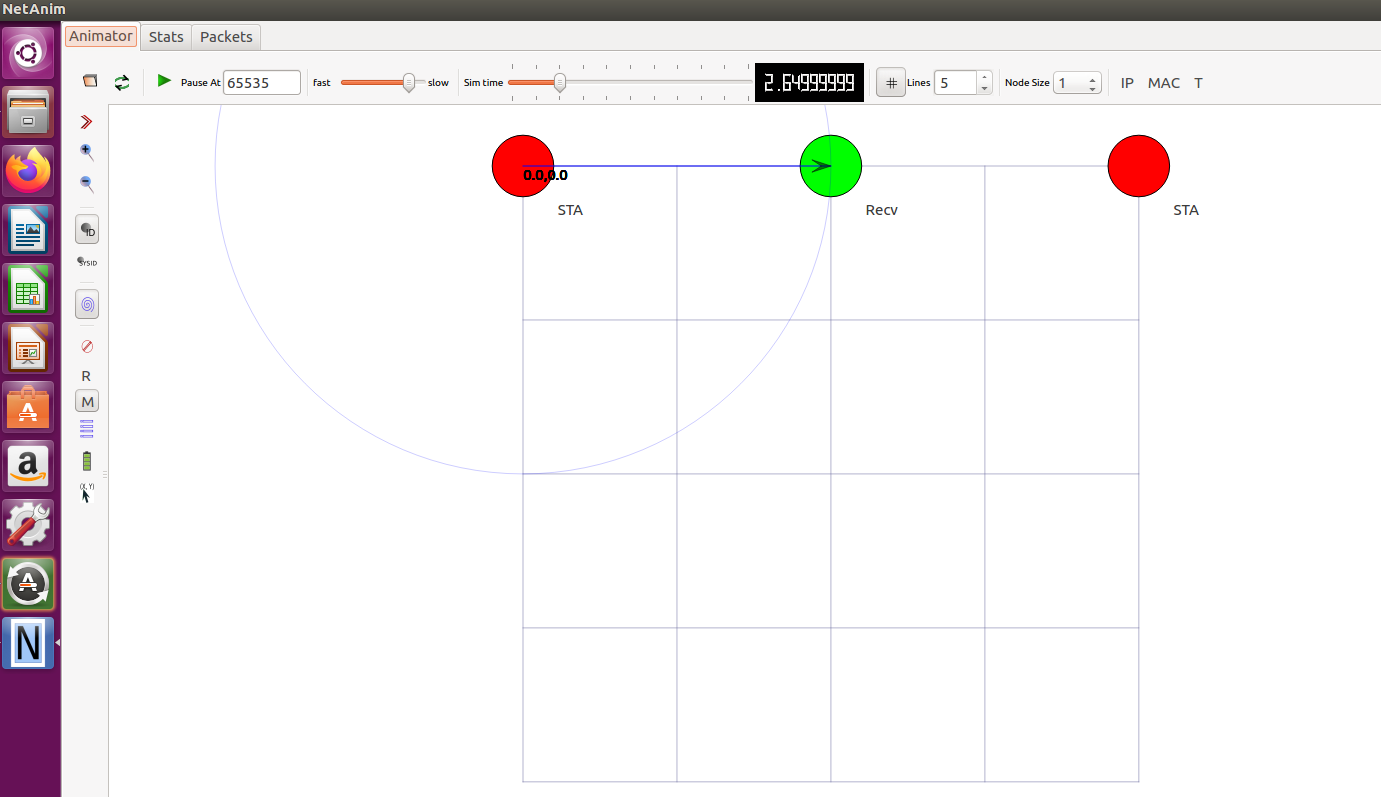
\includegraphics[width=0.9\linewidth]{image/screenshot020}
	\caption{运行画面}
	\label{fig:screenshot020}
\end{figure}

【实验小结】

通过本次实验以及源码阅读我初步知道了如何编写一个ns3脚本来模拟一个预设的网络场景,掌握了科学研究的工具是进行科学研究的第一步。

隐藏节点的问题是计算机网络中经常被拿来讨论的问题,可是只有亲自写过代码清楚其中的逻辑才能完全掌握它。

\subsubsection{2.移动自组网络manet实验}

【实验目标】

实验目标,主要是对移动自组网络的传输机制有一个直观的了解,加深对中间节点路由协议原理的理解,培养学生的初步的观察力和分析能力,形成最基本的研究能力。

【实验原理】

自组网络实验主要是揭示其典型的传输过程。工程上,经常将数据发送节点,称为源(source)节点,主要用于采集数据,接收节点,称为汇聚(sink)节点,将收集到的数据统一发送给数据中心。实验将使用50个节点,其位置随机确定的,其中,确定1个汇聚节点和10个源节点,源节点将同时向汇聚节点发送数据,不能直接传输到达的数据,将由其他中间节点进行路由,实验允许采用OLSR、AODV、DSDV和DSR路由协议,缺省采用AODV路由协议。通过观察数据包传输来理解自组网络运行机制。

AODV无线自组织按需距离矢量协议. 当一个节点需要给网络中的其他节点传送信息时,如果没有到达目标节点的路由,则必须先以组播的形式发出RREQ(路由请求)报文。RREQ报文中记录着发起节点和目标节点的网络层地址,邻近节点收到RREQ,首先判断目标节点是否为自己。如果是,则向发起节点发送RREP(路由回应);如果不是,则首先在路由表中查找是否有到达目标节点的路由,如果有,则向源节点单播RREP,否则继续转发RREQ进行查找。


\begin{figure}[htbp]
	\centering
	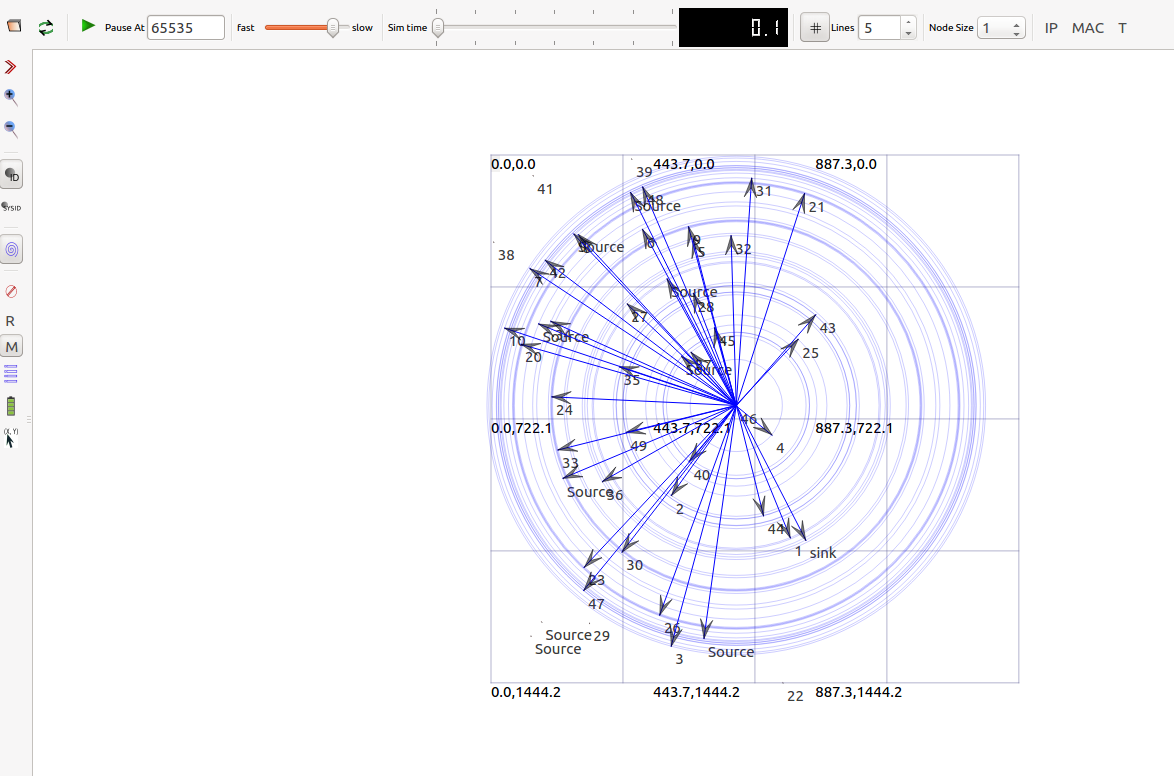
\includegraphics[width=0.8\linewidth]{image/screenshot023}
	\caption{实验界面示意}
	\label{fig:screenshot023}
\end{figure}



【实验内容】

虚拟实验由manet-routing.cc实现。具体步骤:

1、编译manet-routing..cc。

1)复制manet-routing.cc到NS\_HOME/scratch

2)编译manet-routing.cc:./waf –run scratch/ manet-routing.cc

2、运行目标代码。

1)将目录移动到NS\_HOME/scratch/build

2)运行目标代码:./ manet-routing.cc

\begin{figure}[htbp]
	\centering
	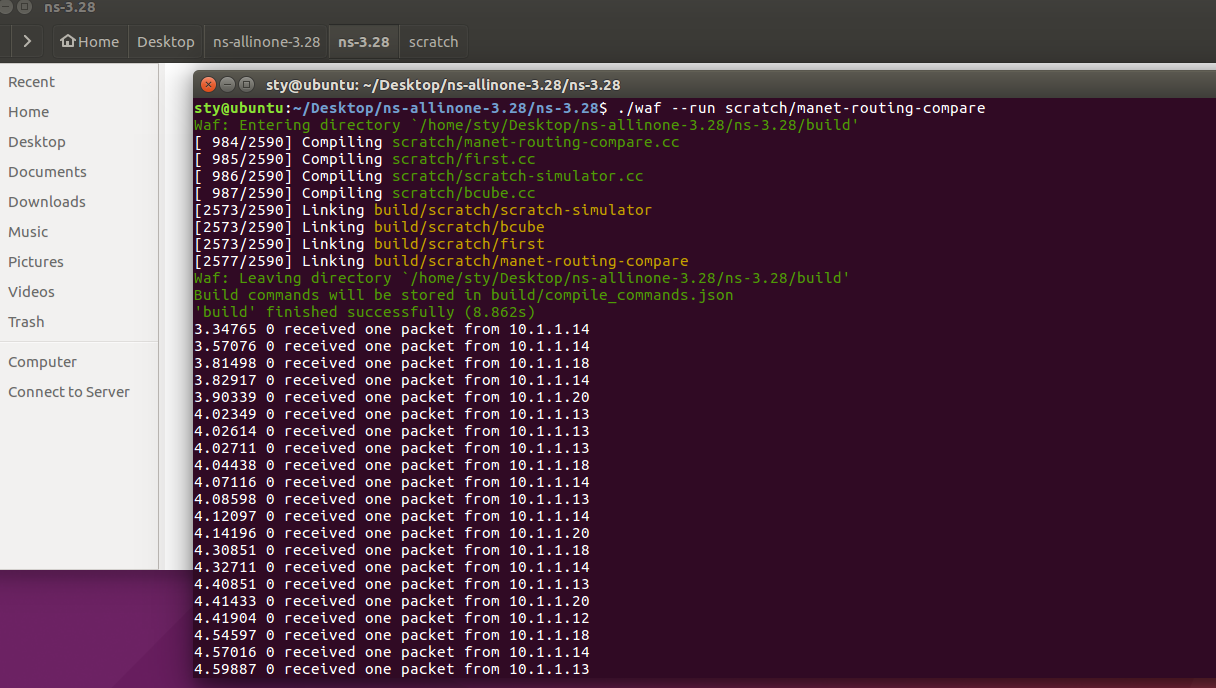
\includegraphics[width=0.8\linewidth]{image/screenshot021}
	\caption{编译并运行manet-routing.cc}
	\label{fig:screenshot021}
\end{figure}


3、显示运行动画

1)将目录移动到执行目录netanim

2)启动netanim动画工具程序:./NetAnim

3)显示运行动画。打开manet-routing.xml

\begin{figure}[htbp]
	\centering
	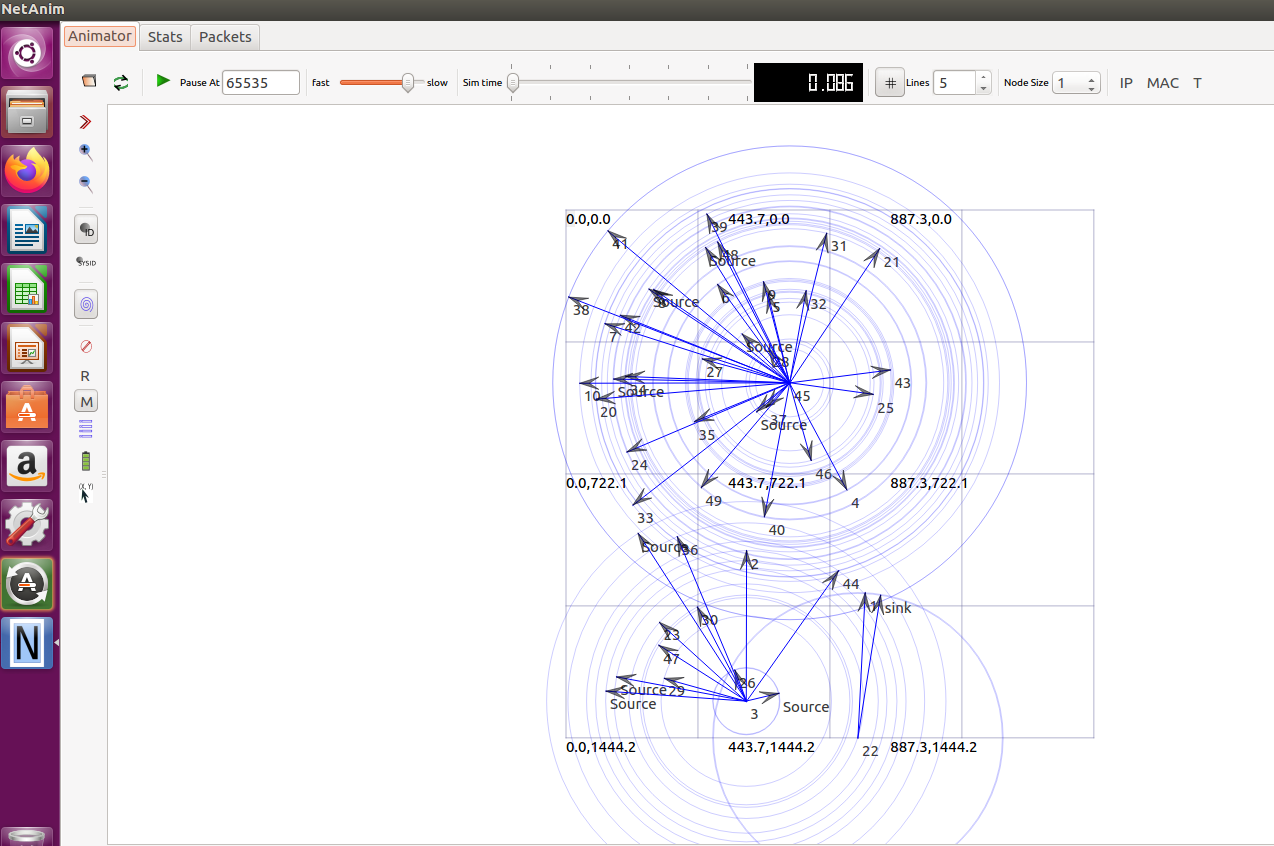
\includegraphics[width=0.9\linewidth]{image/screenshot022}
	\caption{显示运行动画}
	\label{fig:screenshot022}
\end{figure}


【实验小结】

无线自组织网络有非常多的应用情形,这个简单的,非常经典的demo带我入门,领略了ns3的强大之处。

\subsection{实验小结}

通过本次虚拟无线网络实验,初步了解了ns3的使用方法和它的强大之处,也为后续做NS3自选实验做好了铺垫。

第二个实验我特别关注了,在现实中,有很多关于无线自组织网络的研究,例如在本次的自选实验中,我们曾关注过一篇车用自组织网络(VANETs),其中详细介绍了车用自组织网络的工作方法,还基于NS3研究了车用自组织网络的路由协议的性能。较之一般的Ad hoc网络,VANETs的动态特性更为明显。VANETs当中的汽车节点移动速度更快、拓扑变化更频繁、路径寿命更短。同时,VANETs当中的汽车节点移动模型比较复杂,车辆节点密度不均匀等特点也给VANETs的研究工作带来了极大的困难。

\section{静态路由配置实验}
\subsection{实验目的}

静态路由,是指由人工根据网络拓扑结构来创建路由表。路由器需要依靠路由表来转发 IP数据包,该实验是路由器实验中最基础的实验,后续的几个实验都以静态路由为基础。静态路由也是理解路由原理最直观的途径。实验模仿两个远程子网的互联,两个子网在本地各 接一个路由器,路由器之间用远程网络相连,使用静态路由实现远程子网互联。

(1)	深入了解IP路由基本原理。

(2)	了解和掌握配置静态路由配置方法。

\subsection{实验设备}

实验环境由两台路由器、两台计算机和一台交换机组成,模拟两个远程子网互联。使用单根串行交叉线将两个路由器的串口对接起来,代表路由器之间的远程网络;将路由器以太网端口和两台计算机网卡都用网线直接连接到交换机,由交换机担当网络连接;通过串行线将计算机串口com同路由器console口连接起来,两台计算机超级终端将作为路由器管理的操作平台。

\subsection{实验网络拓扑}


\begin{figure}[htbp]
	\centering
	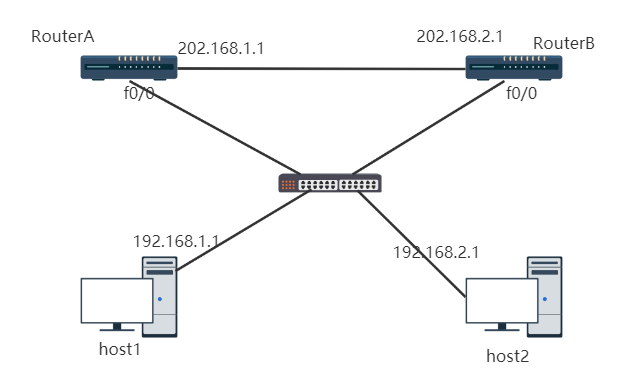
\includegraphics[width=0.7\linewidth]{image/screenshot024}
	\caption{静态路由实验实验网络拓扑}
	\label{fig:screenshot024}
\end{figure}


\subsection{实验内容}

\begin{lstlisting}
1.连接路由器
--打开路由器电源
--使用console线将计算机串口com1与路由器console口直接相连;
--建立HyperTerminal:开始程序附件通讯超级终端名称=router连接=com1Baut Rate=9600,8,no parity, 1 stop bit;
--进入特权模式:router01>en(able) ,Enable Secret Password=cisco
2查看端口状态:
--记录以太0/0口IP地址:router01# sh interface g 0/0
--记录串口0/0口IP地址:router01# sh interface ser 0/0/1
3配置快速以太f0/0
--进入配置模式:router01#config t
--进入以太口:router01(config)#in g0/0
--删除旧IP地址: router01(config-if)#no ip address <ipaddress><subnet mask>
--添加IP地址: router01(config-if)#ip address <ipaddress><subnet mask>
--开启端口功能:router01(config-if)#no shut
4配置串口s0/0
--退到配置模式:router01(config-if)#exit
--进入串口:router01(config)#in s0/0/1
--设置新IP地址
5 静态路由
5.1添加对端路由: router01(config)#ip route 192.168.y.0 255.255.255.0 202.168.1.z # 对端网络地址和广域端口地址;
5.2查看路由表:  router01# sh ip route
5.3 打开路由功能:router01# config t
router01(config)#ip routing
router01(config-if)#exit
5.4 测试
--配置计算机IP地址:192.168.x.254
--测试连通(从计算机):ping 192.168.y.254# 对端计算机
6 缺省路由
6.1删除静态路由: router01(config)#no ip route 192.168.y.0 255.255.255.0 
6.2添加缺省路由: router01(config)#ip route 0.0.0.0 0.0.0.0 202.168.1.z # 对端网络地址和广域端口地址;
6.3查看路由表:router01# sh ip route
6.4 测试
--测试连通(从计算机):ping 192.168.y.254# 对端计算机
7查看运行配置:router01# sh running config

\end{lstlisting}


\begin{figure}[htbp]
	\centering
	\includegraphics[width=0.7\linewidth]{image/1907846D1B5FCD168DC34B37C57127CE}
	\caption{用 sh ip route 查看路由表的照片}
	\label{fig:1907846d1b5fcd168dc34b37c57127ce}
\end{figure}


\begin{figure}[htbp]
	\centering
	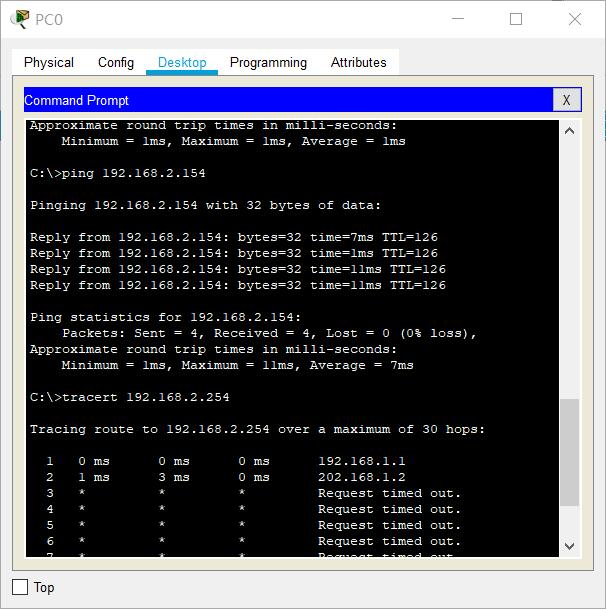
\includegraphics[width=0.7\linewidth]{image/QQ截图20201028235123}
	\caption{用tracert 跟踪路径}
	\label{fig:qq20201028235123}
\end{figure}

\begin{figure}[htbp]
	\centering
	\includegraphics[width=0.7\linewidth]{image/E7210D63DB010B2DDCD3092AFB1AB061}
	\caption{静态路由配置成功,ping通了的照片}
	\label{fig:e7210d63db010b2ddcd3092afb1ab061}
\end{figure}


\subsection{实验小结}

本次实验还是遇到了不少小问题的,在金老师的指导下也收获了不少debug的方法。

1.计网实验教室系统重装过了,防火墙没关,导致一开始ping不通。

2.一开始完成实验操作后并没有ping通两台主机,经过排查,查看路由器路由表的时候发现没有从路由器1到路由器2的路由,但是这个路由应该已经在之前的操作里设置过了,据此断定是因为串口接触不良,串口接触良好后再次查看路由器的路由表,对应的路由就出现了。

3.\textbf{配置时和已有的路由冲突了,使用no命令删除了冲突的IP,最后配置成功。这点很重要!}当时因为冲突报错困扰了我很长时间。

4.许多串口可能接触不良,最后我总结出经验,需要使用no shut命令配合串口旁边的指示灯来判断串口是否正常。

5.接线前先检查包括串口在内的各部件是否工作正常,正常后再进行进一步的实验,以免实验失败了还难以排查问题。

\section{RIP动态路由实验}
\subsection{实验目的}

1.	了解和掌握路由信息协议 RIP 概念;

2.	配置 RIP 动态路由,实现网际通信。

这一讲书上没有写,只能看文档了。

\subsection{实验设备}

两台路由器,使用串行线将两个 0 串口对接;两台计算机作为操作平台;一台交换机担当网络连接。

\subsection{实验网络拓扑}
实验网络拓扑和静态路由是一样的,只不过路由表不用自己设置了。

\begin{figure}[htbp]
	\centering
	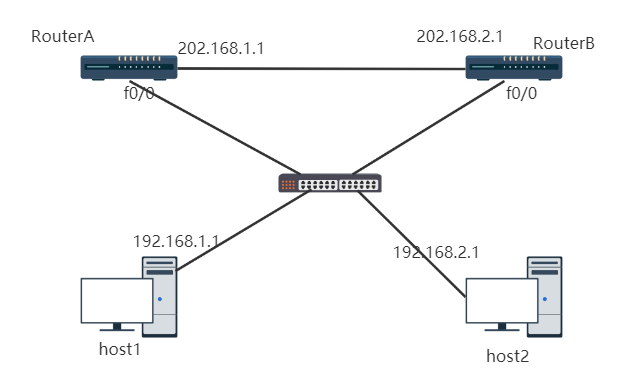
\includegraphics[width=0.7\linewidth]{image/screenshot024}
	\caption{RIP动态路由实验实验网络拓扑}
	\label{fig:screenshot024-2}
\end{figure}

\subsection{实验内容}

\begin{lstlisting}
连接路由器
--打开路由器电源
--使用console线将计算机串口com1与路由器console口直接相连;
--建立HyperTerminal:开始程序附件通讯超级终端名称=router连接=com1Baut Rate=9600,8,no parity, 1 stop bit;
--进入特权模式:router01>en(able) ,Enable Secret Password=cisco
2查看端口状态:router01# sh interface
记录IP地址;
3配置快速以太网f0/0
--进入配置模式:router01#config t
--进入以太口:router01(config)#in f0/0
--删除旧IP地址: router01(config-if)#no ip address <ipaddress><subnet mask>
--添加IP地址: router01(config-if)#ip address <ipaddress><subnet mask>
--开启端口功能:router01(config-if)#no shut
4配置串口s0/0
--退到配置模式:router01(config-if)#exit
--进入串口:router01(config)#in s0/0
--设置IP地址: router01(config-if)#ip addr 202.168.1.1 255.255.255.0
5配置串口s0/1
--退到配置模式:router01(config-if)#exit
--进入串口:router01(config)#in s0/1
--设置IP地址: router01(config-if)#ip addr 202.168.2.1 255.255.255.0
--设置带宽: router01(config-if)#band 256
6 配置RIP动态路由
--添加RIP: router01(config)#router rip #如果路由功能关闭,rip必须重新配置;
--指定邻居网络:router01(config-router)# network 192.168.1.0
router01(config-router)# network 202.168.1.0
router01(config-router)# network 202.168.2.0
--查看RIP路由表:router01# sh ip route rip 
7 测试
--配置计算机IP地址:192.168.x.254
-- router01#no ip domain-lookup
-- router01#trace ip 192.168.2.250
8 跟踪调试
-- router01#debug ip rip#查看信息发送端口
9 被动接口设置 
--进入RIP设置: router01(config)#router rip
--以太网端口配置成被动模式: router01(config-router)#passive-interface f0/0
--查看调试:以太口不再发送

\end{lstlisting}

实验拍照如下图\ref{fig:63f1c6dd39df7a536df3207bdc2cd44}:


\begin{figure}[htbp]
	\centering
	\includegraphics[width=0.7\linewidth]{image/63f1c6dd39df7a536df3207bdc2cd44}
	\caption{RIP动态路由实验截图}
	\label{fig:63f1c6dd39df7a536df3207bdc2cd44}
\end{figure}



\subsection{实验小结}

本次动态路由实验也遇到了一定的问题,在第一次尝试中遇到了线路无法接通的困惑,具体如下:在配置完所有端口后,在两个路由器的四个串口上的指示灯只亮了三展,在router1的s0/0/0口上指示灯是亮的,而在router2的s0/0/0口上指示灯是灭的,并且并不是指示灯坏了,指示灯有时是能断续发一点光的。

实验结果是,利用tracert查看路由,发现包通过了s0/0/1口,也就是限速的串口,并且延迟很高(大约20ms),这说明串口配置确实有问题,这令人百思不得其解。

同时,在计算机网络课程的学习中,我得知了RIP是距离向量路由算法(DVR 计算机网络与因特网第六版P203)的实现,OSPF是链路状态路由协议(LSR 计算机网络与因特网第六版P202)的实现,这让我对动态路由算法的底层原理有了更深入的了解。

\section{OSPF动态路由实验}
\subsection{实验目的}

动态路由是指由软件根据网络拓扑结构自动构建路由表,适合于较大规模网络的路由配置。最难能可贵的是动态路由能自动适应网络故障,一旦发生网络故障,会根据网络故障发生 情况重新生成路由表,及时消除故障的影响。动态路由配置技能是路由器管理的主要工程技能,必须熟悉和掌握。实验模仿两个远程子网的互联,两个子网各接一个路由器,路由器之间用远程网络相连,使用开放式最短路径优先协议(OSPF)实现远程子网互联。

(1)	了解动态路由表生成基本原理。

(2)	了解最短路径优先算法基本思想。

(3)	了解掌握OSPF动态路由技能。


\subsection{实验设备}

实验环境主要由两台路由器、两台计算机和一台交换机组成。使用两根串行交叉线将两个路由器的串口对接起来,创建两个远程传输子网,便于动态路由选择;将路由器以太网端口 和两台计算机网卡都用网线直接连接交换机,由交换机担当网络连接;通过串行线将计算机串口com同路由器console口连接起来,两台计算机超级终端作为路由器管理的操作平台。

\subsection{实验网络拓扑}

实验网络拓扑还是和静态路由是一样的,只不过路由表不用自己设置了。如图\ref{fig:screenshot024-3}所示。

\begin{figure}[htbp]
	\centering
	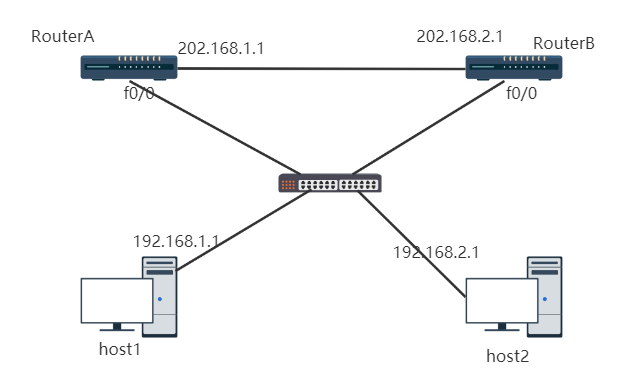
\includegraphics[width=0.7\linewidth]{image/screenshot024}
	\caption{OSPF动态路由实验网络拓扑}
	\label{fig:screenshot024-3}
\end{figure}


\subsection{实验内容}

\begin{lstlisting}
连接路由器
--打开路由器电源
--使用console线将计算机串口com1与路由器console口直接相连;
--建立HyperTerminal:开始程序附件通讯超级终端名称=router连接=com1Baut Rate=9600,8,no parity, 1 stop bit;
--进入特权模式:router01>en(able) ,Enable Secret Password=cisco
2查看端口状态:router01# sh interface
记录IP地址;
3配置快速以太网f0/0
--进入配置模式:router01#config t
--进入以太口:router01(config)#in f0/0
--删除旧IP地址: router01(config-if)#no ip address <ipaddress><subnet mask>
--添加IP地址: router01(config-if)#ip address <ipaddress><subnet mask>
--开启端口功能:router01(config-if)#no shut
4配置串口s0/0
--退到配置模式:router01(config-if)#exit
--进入串口:router01(config)#in s0/0
--设置IP地址: router01(config-if)#ip addr 202.168.1.1 255.255.255.0
5配置串口s0/1
--退到配置模式:router01(config-if)#exit
--进入串口:router01(config)#in s0/1
--设置IP地址: router01(config-if)#ip addr 202.168.2.1 255.255.255.0
--设置带宽: router01(config-if)#band 256
6 配置OSPF动态路由
--添加OSPF: router01(config)#router ospf 100 #如果路由功能关闭,rip必须重新配置;
--指定邻居网络:router01(config-router)# network 192.168.1.0 0.0.0.255 area 0
router01(config-router)# network 202.168.1.0 0.0.0.255 area 0
router01(config-router)# network 202.168.2.0 0.0.0.255 area 0
--查看OSPF ID:router01# sh ip ospf int 
--查看OSPF路由表:router01# sh ip route ospf 
--查看OSPF邻居:router01# sh ip ospf nei
7 测试
--配置计算机IP地址:192.168.x.254
-- router01#no ip domain-lookup
-- router01#trace ip 192.168.2.250
8 跟踪调试
-- router01#debug ip ospf#查看信息发送端口

\end{lstlisting}

\begin{figure}[htbp]
	\centering
	\includegraphics[width=0.7\linewidth]{image/4035bc3b7ac7d1a0c09d9908097465f}
	\caption{OSPF实验拍照}
	\label{fig:4035bc3b7ac7d1a0c09d9908097465f}
\end{figure}


\subsection{实验小结}

本次的实验是和RIP路由一起做的。

在第一次尝试中遇到了线路无法接通的困惑,具体如下:在配置完所有端口后,在两个路由器的四个串口上的指示灯只亮了三展,在router1的s0/0/0口上指示灯是亮的,而在router2的s0/0/0口上指示灯是灭的,并且并不是指示灯坏了,指示灯有时是能断续发一点光的。
实验结果是,利用tracert查看路由,发现包通过了s0/0/1口,也就是限速的串口,并且延迟很高(大约20ms),这说明串口配置确实有问题,这令人百思不得其解。

同时,在计算机网络课程的学习中,我得知了RIP是距离向量路由算法(DVR 计算机网络与因特网第六版P203)的实现,OSPF是链路状态路由协议(LSR 计算机网络与因特网第六版P202)的实现,这让我对动态路由算法的底层原理有了更深入的了解。

\section{帧中继配置实验}
\subsection{实验目的}

广域网是另一类主要有线物理网络,可以实现跨地域的网络连接,承担着骨干传输网络作用,只有ISP(Internet Service Provider,互联网服务提供商)才会拥有,如中国电信、移动等,普通企业很难见到此类设备。因此本书没有对广域网进行详尽介绍,但了解广域网网络和局域网互联,有助于深入理解网际网的异构特性。本实验利用路由器模拟帧中继交换机,用于远程连接两个以太网,实现网络互联。

(1)	了解广域网基本概念。

(2)	区分二层路由和三层路由基本概念。

(3)	熟悉帧中继交换机永久虚电路及配置步骤。

\subsection{实验设备}

实验环境主要由三台路由器、三台计算机和一台交换机组成,模拟一个由局域网和广域网组成的网际网。路由器(模拟帧中继交换机)使用单根串行交叉线将路由器A和路由器C的 广域网串口连接起来,路由器B和路由器C的广域网串口连接起来(构建帧中继网络专线以连接两个远程子网),并使得同RouterC相连的电缆连接线类型均为DCE,将路由器A和路由 器B以太网端口和两台计算机网卡都用网线直接连接到交换机,由交换机担当网络连接;通过串行线将各个计算机串口com同路由器console口连接起来,使用各自超级终端作为路由器管理的操作平台。

\subsection{实验网络拓扑}


实验网络拓扑如图\ref{fig:screenshot025}

\begin{figure}[htbp]
	\centering
	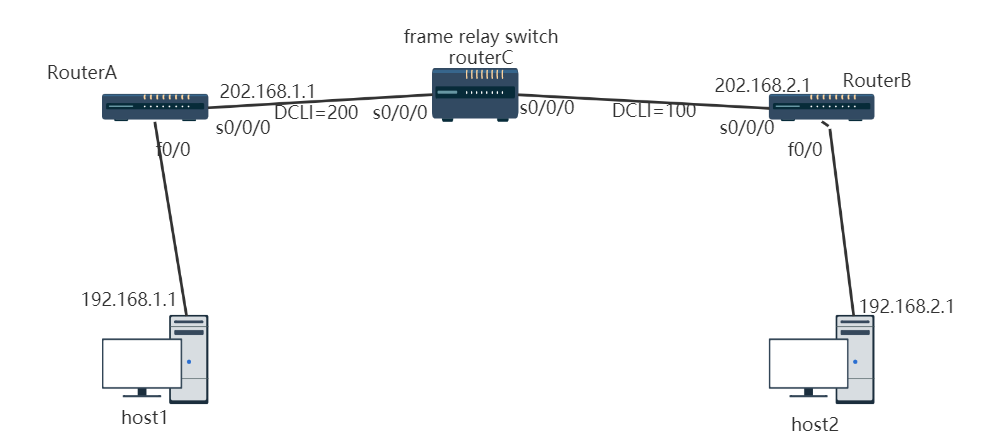
\includegraphics[width=0.7\linewidth]{image/screenshot025}
	\caption{帧中继实验网络拓扑}
	\label{fig:screenshot025}
\end{figure}


\subsection{实验内容}

\begin{lstlisting}
1. 帧中继交换机配置
1.1路由器设置成帧中继交换机
--进入全局配置模式: router03#config t
--启用作为帧中继交换机:router03(config)#frame switching
--查看帧中继功能:router03#sh run
1.2 设置s0/0端口
--查看端口物理连接:router03#sh control s0/0#检查端口s0/0, s0/1,物理线是否连接,
--设置端口:router03 (config)#in s0/0#端口s0/0
--封装端口为Frame:router03 (config-if)#encap   frame#enacapsulation frame-relay 
--帧封装方式:router03 (config-if)#fram intf-type dce 
--设置lmi类型:router03 (config-if)#fram lmi-type cisco 
--时钟频率:router03 (config-if)#clock rate 56000
--配置广域路由(pvc):router(config-if)#fram route 200 inter s0/1 100
--启动端口:router03 (config-if)#no shut
router03 (config-if)# exit
1.3设置s0/1端口:
--设置端口:router03 (config)#in s0/1#端口s0/1
--封装端口为Frame:router03 (config-if)#encap   frame#enacapsulation frame-relay 
--配置端口类型DCE:router03 (config-if)#fram intf-type dce 
--设置lmi类型:router03 (config-if)#fram lmi-type cisco 
--时钟频率:router03 (config-if)#clock rate 56000
--配置广域路由(pvc):router03 (config-if)#fram route 100 inter s0/0 200
1.4 检查帧中继交换机
--查看配置:router03#sh run
--查看交换机路由表,即pvc构成:router03#sh frame route
\end{lstlisting}

\begin{table}[htbp]

\centering
\begin{tabular}{|l|l|l|l|}
	\hline IN\_Port & IN\_DLCl & OUT\_Port & OUT\_DLCl \\
	\hline $\mathrm{S} 0 / 0$ & 200 & $\mathrm{~S} 0 / 1$ & 100 \\
	\hline $\mathrm{S} 0 / 1$ & 100 & $\mathrm{~S} 0 / 0$ & 200 \\
	\hline
\end{tabular}
\caption{查看交换机路由表,即pvc构成}
\end{table}
\begin{lstlisting}
--查看pvc使用情况:router03#sh frame pvc#端口类型DCE,DLCI用途是Switching,激活状态
2 路由器router01配置
2.1配置快速以太网f0/0
--进入配置模式:router01#config t
--进入以太口:router01(config)#in f0/0
--删除旧IP地址: router01(config-if)#no ip address <ipaddress><subnet mask>
--添加IP地址: router01(config-if)#ip address <ipaddress><subnet mask>
--开启端口功能:router01(config-if)#no shut
2.2 配置帧中继广域网链路
--查看pvc链路号:router01#sh frame pvc#看不到
--设置端口:router01(config)#in s0/0#端口s0/0
--封装端口为Frame:router01(config-if)#encap  frame#线路才启用; 
--查看并记录DLCI编号:router01#sh frame pvc
--设置lmi类型:router01(config-if)#fram lmi-type cisco 
--设置IP地址:router01(config)#ip addr 202.168.2.1 255.255.255.0 
--启动端口:router01(config-if)#no shut
2.3 地址映射管理
--查看DLCI同IP地址映射状态:router01#sh frame map#已经映射就不用设立;
2.4 静态路由配置
--添加缺省路由: router01(config)#ip route 0.0.0.0 0.0.0.0 202.168.2.2 # 对端广域端口地址;
--或添加静态路由: router01(config)#ip route 192.168.y.0 255.255.255.0 202.168.2.2 
--查看路由表:router01# sh ip route
2.5 测试
--配置计算机IP地址:192.168.x.254
--测试连通(从计算机):ping 192.168.y.254# 对端计算机
2.6 静态建立帧中继映射
--关闭动态反向地址解析:router01(config)#int s0/0#指定端口
router01(config-if)#no fram inverse
router01(config-if)#shut#重启端口
router01(config-if)#no shut
--查看DLCI同IP地址映射状态:router01#sh frame map#不存在映射
--建立映射DLCI:router01(config-if)#fram map ip 202.168.2.2 200#对端地址 
2.7 重新测试
--配置计算机IP地址:192.168.x.254
--测试连通(从计算机):ping 192.168.y.254# 对端计算机

\end{lstlisting}

\subsection{实验小结}

这个实验遇到的主要问题还是实验设备的问题!串口容易坏或者接触不良!两个路由器的两个串口灯都是亮的,但是并不通,得用手去按紧了才通。

这个实验本身还是比较复杂的,在做实验的时候也做了很久才做出来。我本来还想再cisco packet tracer上重现这个实验加深一下印象,但是在执行frame switching的命令的时候找不到frame命令,后来一查才知道cisco packet tracer不支持这个命令。

做了这个实验之后更加深入的理解了帧中继技术,也更加掌握了其路由表的建立的机制。

\section{组播实验}
\subsection{实验目的}

组播是一对多的传输模式,即一个节点向组播地址发送一个IP数据包,所有该组播的成员 都将接收这个IP数据包,具有较高传输效率。组播应用非常广泛,视频会议就是组播的典型应 用,正确使用组播对于提高网络传输效率非常有价值。但组播不会自动跨域子网,需要对路由器 进行适当设置。实验模仿两个远程子网的互联,两个子网各接一个路由器,路由器之间用远程网 络相连,安排一个组播发送节点和两个组播接收节点,配置路由器使得组播能跨越子网。

(1)了解组播协议基本原理。

(2)掌握路由器组播配置技能。

\subsection{实验设备}

实验环境主要由两台路由器、三台计算机和两台交换机组成。使用单根串行交叉线将路 由器A同路由器B的串口对接起来,模拟远程传输网络;将路由器A以太网端口和主机 Host1用网线直接连接到一个交换机Switch1;将路由器B以太网端口和主机Host2和Host3 用网线直接连接到另一个交换机Switch2;按图4-54通过串行线将主机Hostl和Host2串口 com同路由器console 口连接起来,使用超级终端充当路由器管理的操作平台。运行组播测试工具软件用于组播测试。

\subsection{实验网络拓扑}

实验网络拓扑如图\ref{fig:screenshot026}所示
\begin{figure}[htbp]
	\centering
	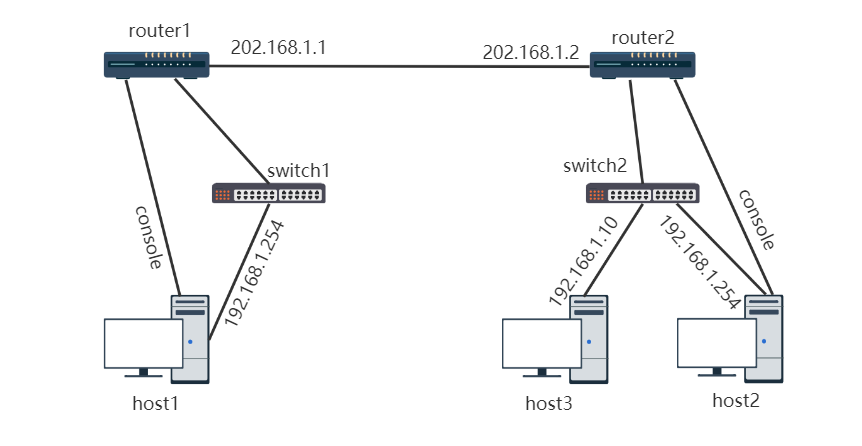
\includegraphics[width=0.7\linewidth]{image/screenshot026}
	\caption{实验网络拓扑}
	\label{fig:screenshot026}
\end{figure}

\subsection{实验内容}

\begin{lstlisting}
1.连接路由器
--打开路由器电源
--使用console线将计算机串口com1与路由器console口直接相连;
--建立HyperTerminal:开始程序附件通讯超级终端名称=router连接=com1Baut Rate=9600,8,no parity, 1 stop bit;
--进入特权模式:router01>en(able) ,Enable Secret Password=cisco
2查看端口状态:
--记录以太0/0口IP地址:router01# sh interface fast 0/0
--记录串口0/0口IP地址:router01# sh interface ser 0/0
3配置快速以太f0/0
--进入配置模式:router01#config t
--进入以太口:router01(config)#in f0/0
--删除旧IP地址: router01(config-if)#no ip address <ipaddress><subnet mask>
--添加IP地址: router01(config-if)#ip address <ipaddress><subnet mask>
--开启端口功能:router01(config-if)#no shut
--开启端口功能:router01(config-if)#no shut
4配置串口s0/0
--退到配置模式:router01(config-if)#exit
--进入串口:router01(config)#in s0/0
--设置新IP地址
5 静态路由
5.1添加对端路由: router01(config)#ip route 192.168.y.0 255.255.255.0 202.168.1.z # 对端网络地址和广域端口地址;
5.2查看路由表:router01# sh ip route
5.3 测试组播不成功
--配置计算机IP地址:McastSend.exe
--测试连通(从计算机):MCastReiver.exe# 对端计算机
6 配置组播
6.1开启组播功能: router01(config)#ip multicast-routing 
6.2配置串口组播方式: router01(config)#int s0/0/0 # 对端网络地址和广域端口地址;
router01(config-if)#ip pim dense-mode # 
6.3配置以他口组播方式:router01(config)#int  f0/0 # 对端网络地址和广域端口地址;
router01(config-if)#ip pim dense-mode # 
6.4查看组播:router01# sh ip mroute
router01# sh ip pim inyter
router01# sh ip pim nei

--测试连通(从计算机): 192.168.y.254# 对端计算机
7查看运行配置:router01# sh running config

\end{lstlisting}

实验截图如下图\ref{fig:screenshot027}:


\begin{figure}[htbp]
	\centering
	\subfigure[组播测试发送端]{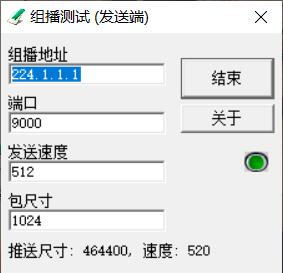
\includegraphics[height=0.4\linewidth]{image/screenshot027}}
	\subfigure[组播测试接收端]{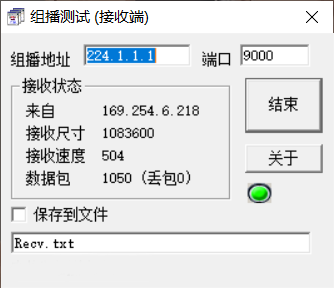
\includegraphics[height=0.4\linewidth]{image/screenshot028}}
	\caption{组播测试截图}
	\label{fig:screenshot027}
\end{figure}



\subsection{实验小结}



这个实验遇到的主要问题还是出现在设备上,在前面的几次基础实验的成功经验下才排除了错误。串口容易坏或者接触不良!两个路由器的两个串口灯都是亮的,但是并不通,得用手去按紧了才通。

实验中使用命令 netsh interface ipv4 show join 查看组播是否运行在了正确的网卡上!最好在适配器设置里将无关的网卡禁用以提高成功率。

本次实验中的路由配置不一定是静态路由,也可以选用RIP或者OSPF动态路由,IP地址分配也可以是DHCP分配,只不过要自己去查看分配到的IP地址,只要保证两个字网可以互相连通就可以了。在保证上述前提下,软件程序运行在正确的网卡的前提下,实验做成功还是比较容易的。

\section{动态IP地址分配DHCP实验}
\subsection{实验目的}

IP地址在人工配置中极易造成重复,从而发生冲突,动态主机配置协议(Dynamic Host Configuration Protocol,DHCP),将自动为子网内的节点向卡分配IP地址。DHCP可以简化网络地址配置,适合非专业人员使用,目前很多网络设备都具备DHCP服务功能,如家庭无线猫也使用DHCP。实验通过开启路由器的DHCP功能,对连接同一个交换机的主机开展动态地址分配。

(1)	深入了解动态主机配置协议原理。

(2)	了解和掌握DHCP服务的配置步骤。

\subsection{实验设备}

实验设备主要由一台路由器、两台计算机和一台交换机组成。路由器将担当DHCP服务器;将路由器以太网端口和两台计算机网卡都用网线直接连接到交换机,由交换机担当网络连 接;通过串行线将计算机Hostl串口 com同路由器console口连接起来,使用超级终端作为路由器管理的操作平台,两台计算机都作为地址分配实验主机。假如没有路由器和交换机设备,也可以用家用无线路由器来代替。

\subsection{实验网络拓扑}


拓扑图如图\ref{fig:DHCP}所示
\begin{figure}[htbp]
	\centering
	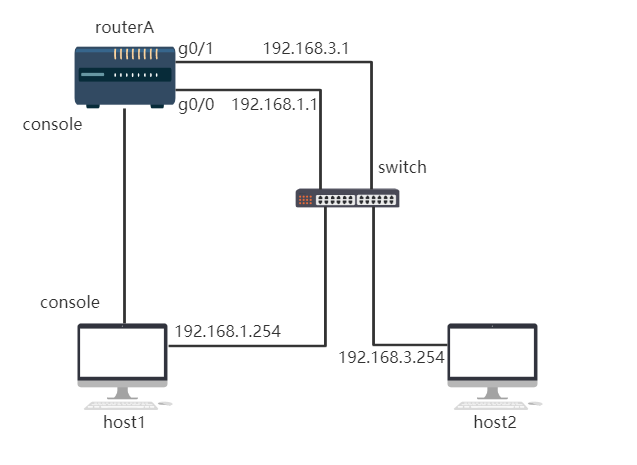
\includegraphics[width=0.7\linewidth]{image/screenshot014}
	\caption{DHCP实验网络拓扑}
	\label{fig:DHCP}
\end{figure}

\subsection{实验内容}
按照实验环境要求,完成实验拓扑结构连接,并打开相关设备电源。

(1)配置RouterA的DHCP服务。使用超级终端,进行网关设置和DHCP服务配置。

1.进入配置模式。

进入特权模式:routerA>en, Enable Secret Password= cisco

进入配置模式:routerA>config t

2.网关设置。

进入以太网端口配置模式:routerA(config) \# in g0/0

设置 IP 地址:routerA(config-if) \# ip address 192. 168. 1. 1 255. 255. 255. 0

开启端口 : routerA(config-if) \# no shut

退出端口配置模式,使端口配置生效:routerA(config-if) \# exit

3.配置DHCP服务。

进入 DHCP 服务配置模式:routerA(config) \# ip dhcp pool mydhcp

设置待可分配网络地址:routerA (dhcp-config) \# network 192. 168. 1. 0 255. 255. 255. 0

域名设置:routerA (dhcp-config) \# domain-name networklab. com

默认网关地址分配设置:routerA(dhcp-config) \# default-router 192. 168. 1. 1

本地 DNS 服务器地址分配设置:routerA(dhcp-config) \# dns-server 202. 120. 190. 208

设置租期:routerA(dhcp-config) \# lease infinite

设置不参与分配地址:routerA(config) \# ip dhcp excluded-address 192.168. 1.1 192. 168.1. 7关闭DHCP冲突日志,以免显示影响操作:routerA(config) \# no ip dhcp conflict logging 启动 DHCP服务:routerA(config) \# service dhcp

退出配置模式,使配置生效:routerA(config)\# exit

(2)配置Hostl网卡地址自动分配设置。

1.设置主机Hosl网卡IP地址自动获取,选择"Internet协议版本4”->“属性”。 选择“自动获得IP地址”和“自动获得DNS服务器地址”->“确定”。

2.査看主机Hostl的IP地址分配状态。打开命令行窗口。 释放分配地址:ipconfig /release

重新申请分配:ipconfig /renew

查看已分配的主机Hostl网卡IP地址:ipconfig /all, IP地址得到了分配,地址为192. 168.1.21,子网掩码为255. 255. 255.0,默认网关地址为192. 168. 1. 1,本地DNS服务器地址 为202. 120. 190. 208,对照配置,完全一致。 


\begin{figure}[htbp]
	\centering
	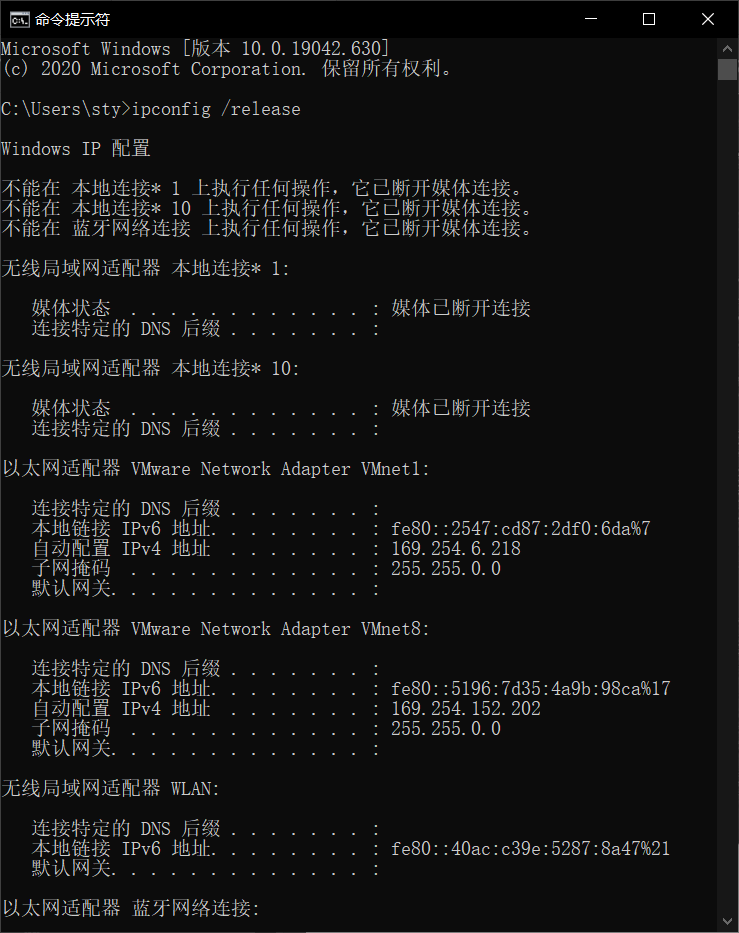
\includegraphics[width=0.7\linewidth]{image/screenshot029}
	\caption{查看主机IP地址分配}
	\label{fig:screenshot029}
\end{figure}

\subsection{实验小结}

DHCP实验是非常简单的实验了,在实验过程中没有遇到问题,在做过DHCP动态IP地址分配协议实验之后对DHCP有了更深的理解,知道家里用的家用路由器是怎么分配IP地址的了。

\section{ACL访问控制实验}
\subsection{实验目的}

包过滤机制是路由器基本处理机制,加入过滤规则,可以实施基本的网络安全控制。阻隔 访问敏感网站和关键主机,均可以使用访问控制列表作为过滤规则实施。学习访问控制列表, 不但可以了解基本网络安全知识,而且还可以提高路由器使用水平。本实验利用路由器的访 问控制列表功能,使得特定的IP地址不能访问,实现网络安全管理任务。

(1)	了解路由器包过滤基本原理。

(2)	了解访问控制列表实施原理。

(3)	利用控制列表实施网络安全。

(4)	掌握访问控制组配置。

(5)	实施包过滤,有选择地允许某些地址组进行网际通信。

\subsection{实验设备}

实验环境主要由两台路由器、两台计算机和一台交换机组成。使用单根串行交叉线将两个路由器的串口对接起来;将路由器以太网端口和两台计算机网卡都用网线直接连接到交换机,由交换机担当网络连接;通过串行线将计算机串口com同路由器console口连接起来,两台计算机超级终端作为路由器管理的操作平台。

\subsection{实验网络拓扑}


\begin{figure}[htbp]
	\centering
	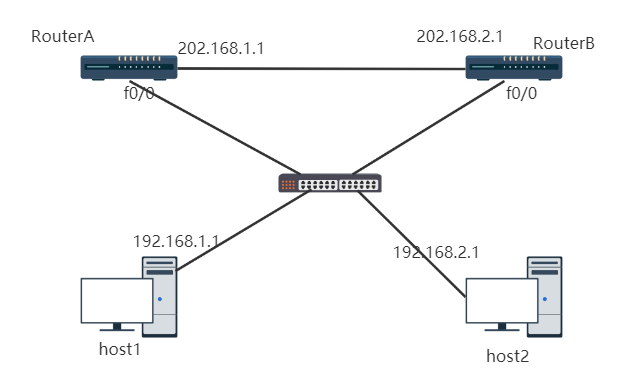
\includegraphics[width=0.7\linewidth]{image/screenshot024}
	\caption{ACL访问控制列表实验网络拓扑}
	\label{fig:acl}
\end{figure}

\subsection{实验内容}

\subsubsection{一、连接路由器}

--打开路由器电源

--使用console线将计算机串口com1与路由器console口直接相连;

--建立HyperTerminal:开始程序附件通讯超级终端名称=router连接=com1Baut Rate=9600,8,no parity, 1 stop bit;

--进入特权模式:router01>en(able) ,Enable Secret Password=cisco

\subsubsection{二、静态路由配置}

2.1 配置快速以太f0/0

--进入配置模式:router01\#config t

--进入以太口:router01(config)\#in f0/0

--删除旧IP地址: router01(config-if)\#no ip address <ipaddress><subnet mask>

--添加IP地址: router01(config-if)\#ip address <ipaddress><subnet mask>

--开启端口功能:router01(config-if)\#no shut

2.2配置串口s0/0

--退到配置模式:router01(config-if)\#exit

--进入串口:router01(config)\#in s0/0

--添加IP地址: router01(config-if)\#ip address <ipaddress><subnet mask>

--开启端口功能:router01(config-if)\#no shut

2.3 静态缺省路由

--添加对端路由: router01(config)\#ip route 0.0.0.0 0.0.0.0 202.168.1.z \# 对端网络地址和广域端口地址;

\begin{figure}[htbp]
	\centering
	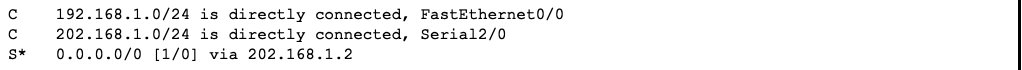
\includegraphics[width=0.7\linewidth]{image/screenshot030}
	\caption{router01的路由表}
	\label{fig:screenshot030}
\end{figure}

\begin{figure}[htbp]
	\centering
	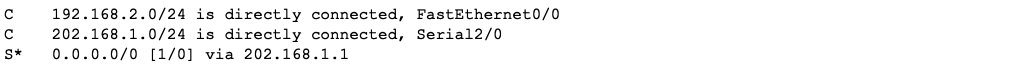
\includegraphics[width=0.7\linewidth]{image/screenshot031}
	\caption{router02的路由表}
	\label{fig:screenshot031}
\end{figure}


\begin{figure}[htbp]
	\centering
	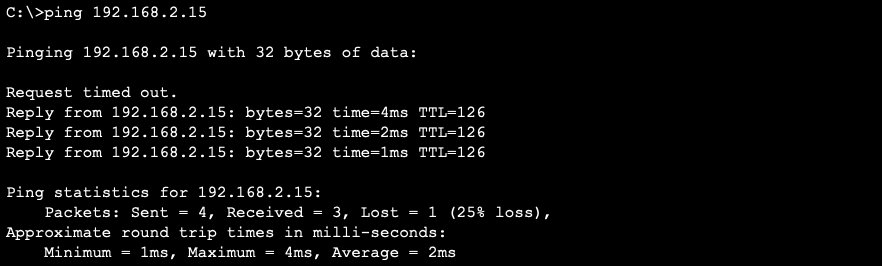
\includegraphics[width=0.7\linewidth]{image/screenshot032}
	\caption{host测试,用ping连通192.168.2.15,成功连通}
	\label{fig:screenshot032}
\end{figure}


\subsubsection{三、访问控制组,只允许内部地址外出}

4.只允许内部地址外出permit:192.168.1.0/28

--192.168.x.15可以外出;

--192.168.x.17不可以外出;

4.1 建立访问控制组

--进入配置模式:router01\#config t

--建立访问控制组1:router01(config)\# access-list 1 permit 192.168.x.0  0.0.0.15

--查看访问控制组:router01\# sh access-list

\begin{figure}[htbp]
	\centering
	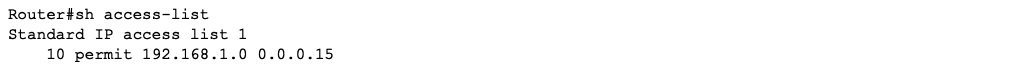
\includegraphics[width=0.7\linewidth]{image/screenshot033}
	\caption{router01的访问控制组}
	\label{fig:screenshot033}
\end{figure}


4.2实施包过滤1

--指定以太端口:router01\# config t

router01(config)\#in f0/0

--建立映射:router01(config)\# ip access-group 1 in 

--查看包过滤:router01\# sh run

\begin{figure}[htbp]
	\centering
	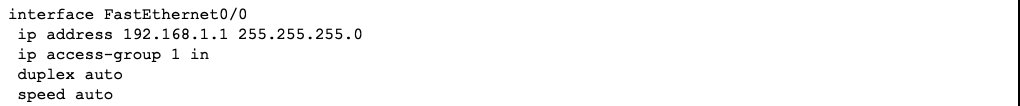
\includegraphics[width=0.7\linewidth]{image/screenshot034}
	\caption{查看包过滤}
	\label{fig:screenshot034}
\end{figure}


4.3 host测试(DOS窗口)

--测试连通(从计算机):ping 192.168.y.1\# 对端路由器,成功

\begin{figure}[htbp]
	\centering
	\includegraphics[width=0.7\linewidth]{image/screenshot035}
	\caption{第一次测试}
	\label{fig:screenshot035}
\end{figure}


--修改计算机IP地址:192.168.x.17

--测试连通(从计算机):ping 192.168.y.1\# 对端路由器,不成功

\begin{figure}[htbp]
	\centering
	\includegraphics[width=0.7\linewidth]{image/screenshot036}
	\caption{修改IP为192.168.1.17后,第二次测试}
	\label{fig:screenshot036}
\end{figure}


4.4实施包过滤2

--指定实施端口:router01\# config t

router01(config)\#in f0/0

--删除映射:router01(config)\# no ip access-group 1 in 

--查看包过滤:router01\# sh run

\begin{figure}[htbp]
	\centering
	\includegraphics[width=0.7\linewidth]{image/screenshot037}
	\caption{删除映射后查看包过滤}
	\label{fig:screenshot037}
\end{figure}


--指定串行端口:router01\# config t

router01(config)\#in s0/0

--建立映射:router01(config)\# ip access-group 1 out


\begin{figure}[htbp]
	\centering
	\includegraphics[width=0.7\linewidth]{image/screenshot038}
	\caption{建立映射后查看包过滤}
	\label{fig:screenshot038}
\end{figure}

\subsubsection{四、访问控制组,只允许外部地址进入}

5(可选)只允许外部地址进入permit:192.168.y.0/28

--192.168.2.15可以进入;

--192.168.2.17不可以进入;

5.1 建立访问控制组

--进入配置模式:router01\#config t

--建立访问控制组1:router01(config)\# access-list 2 permit 192.168.2.0  0.0.0.15 

--查看访问控制组router01\#sh access-list

\begin{figure}[htbp]
	\centering
	\includegraphics[width=0.7\linewidth]{image/screenshot039}
	\caption{router01的访问控制组}
	\label{fig:screenshot039}
\end{figure}


5.2实施包过滤

--实施端口:router01\# config t

router01(config)\#in s0/0

--建立映射:router01(config)\# ip access-group 2 in 

--查看包过滤:router01\# sh run

\begin{figure}[htbp]
	\centering
	\includegraphics[width=0.7\linewidth]{image/screenshot040}
	\caption{查看包过滤}
	\label{fig:screenshot040}
\end{figure}


5.3 测试

--配置对端计算机IP地址:192.168.x.17

--测试连通(从对端计算机):ping 192.168.y.1\# 对端路由器,成功


\begin{figure}[htbp]
	\centering
	\includegraphics[width=0.7\linewidth]{image/screenshot041}
	\caption{第一次测试,成功}
	\label{fig:screenshot041}
\end{figure}

--测试连通(从对端计算机):ping 192.168.y.17\# 对端路由器,不成功

\begin{figure}[htbp]
	\centering
	\includegraphics[width=0.7\linewidth]{image/screenshot042}
	\caption{第二次测试,不成功}
	\label{fig:screenshot042}
\end{figure}


6 查看

--查看运行状态: router01\# show run

\begin{figure}[htbp]
	\centering
	\includegraphics[width=0.7\linewidth]{image/screenshot043}
	\caption{查看运行状态}
	\label{fig:screenshot043}
\end{figure}

--查看访问控制组: router01\# show access-list 1

\begin{figure}[htbp]
	\centering
	\includegraphics[width=0.7\linewidth]{image/screenshot044}
	\caption{查看访问控制组}
	\label{fig:screenshot044}
\end{figure}


router01\# show access-list 2

--删除: router01(config) no access-list 1

--测试连通(从计算机):ping 192.168.y.254\# 对端计算机

\begin{figure}[htbp]
	\centering
	\includegraphics[width=0.7\linewidth]{image/screenshot045}
	\caption{测试:成功}
	\label{fig:screenshot045}
\end{figure}



\subsection{实验小结}

我们都知道我国的防火长城就是由ACL访问控制列表来实现的,所以访问在ACL访问控制列表中的站点的时候需要使用代理服务器。通过这次实验我加深了对访问控制的具体流程的理解,对计算机网络也更感兴趣了。

有前面的很多实验做基础,我已经对连线和路由器、交换机配置等基本操作都很熟悉,实验顺畅的进行。ACL控制访问列表实验是个基于静态路由配置的实验,其网络拓扑结构与前面的很多实验完全相同。通过本次实验掌握了访问控制组的相关配置指令,认识了路由器包过滤机制,也更加深了对网络安全的理解。

\section{邮件收发实验}
\subsection{实验目的}

电子邮件是目前人们工作和个人进行沟通交流的主要渠道,已成为人们生活和工作的重 要组成部分,也是互联网应用最广的服务之一。了解电子邮件原理,可以更有效地开展邮件应 用。实验通过安装邮件服务器,创建一个邮件应用环境,然后使用Telnet工具,使用命令行操 作进行简单邮件的收发。

(1)	了解应用层数据规范和交互命令基本组成。

(2)	了解电子邮件运行的基本模型。

(3)	了解邮件服务器基本安装和管理步骤。

(4)	了解邮件发送交互方式,熟悉SMTP协议消息。

(5)	了解邮件接收交互方式,熟悉POP协议消息。

\subsection{实验设备}

使用一台计算机作为实验运行平台,实验环境主要由软件环境担当。

(1)	启动包含SMTP和POP服务器的邮件服务器,并开设实验邮件账号供实验使用;

(2)	创建networklab. com作为邮箱服务器伪域名;

(3)	使用Telnet T具软件作为客户机,分别访问SMTP服务器和POP服务器,进行邮件 的发送和接收。

\subsection{实验内容}

\subsubsection{实验一:SMTP邮件发送实验}
(1)启动hMailServer服务。打开系统服务管理,“开始”->“系统”->“其他管理工具”-> “管理工具”->“服务”。
如果hMailServer还没启动,右击hMailServer->“启动”。

(2)使用Telnet发送邮件。

1.进入Telnet命令。打开命令行窗口。

输入“telnet",进入Telnet交互模式。

2.连接SMTP服务器,端口号是25

输入"open networklab. com 25"。

3.向邮箱student1@networklab. com发送邮件消息。使用SMTP消息向邮箱student1 @networklab. com发送邮件,具体消息含义参见SMTP消息介绍,数字开头是服务器的响应状态码。

标识发件人身份,HELO networklab. com

指定发件人邮箱,MAIL FROM:jinweizu@163. com

指定收件人邮箱 JRCPT TO:student1@networklab. com

输入信件主体:

DATA

Subject: test SMTP.

结束信件输入:<cr><LF>. <cr><LF>,使用<回车>.<回车>

结束连接:QUIT。

\subsubsection{实验二:POP邮件接收实验}

(1)使用Telnet接收邮件。

1.连接POP服务器,端口号是110

open networklab. com 110

2.接收实验一发送的邮件。通过发送POP消息,接收实验一发送的邮件,数字开头是服务器的响应状态码。

输入邮件账号和口令:

USER studentl©networklab. com

PASS password 

查看当前信件列表:LIST

阅读编号为1的信件内容:RETR1,可以看到实验一发送的邮件内容,邮件成功接收。 结束连接:QUIT。


\begin{figure}[htbp]
	\centering
	\includegraphics[width=0.9\linewidth]{"image/reveive email"}
	\caption{实验截图:成功收到邮件并阅读邮件内容!}
	\label{fig:reveive-email}
\end{figure}


\subsection{实验小结}

邮件收发实验是我认为最好玩的一个应用层协议的实验之一,为此我还在阿里云注册了一个域名imsty.cn并按照与书上相似的方法配置了一个邮件服务器,并成功与我的QQ邮箱进行了邮件发送与接收。

当然在实验中我还遇到了一些困难,比如在我连接smtp服务器的25端口的时候有时候会拒绝连接,后来经过自己查看hMailServer的设置之后发现是如果多次输错密码hMailServer会把那个IP加入黑名单并持续一段时间,在我关闭掉这个设置之后实验成功进行。

在课外我还注册了一个域名,配置了一个邮件服务器,并能成功做到和我的QQ邮箱收发邮件,下面是一些截图。

\begin{figure}[htbp]
	\centering
	\includegraphics[width=0.6\linewidth]{image/screenshot046}
	\caption{发送成功}
	\label{fig:screenshot046}
\end{figure}

\begin{figure}[htbp]
	\centering
	\includegraphics[width=0.6\linewidth]{image/screenshot047}
	\caption{接收成功}
	\label{fig:screenshot047}
\end{figure}



\section{ARP消息分析实验}
\subsection{实验目的}

IP数据包在封装到以太网帧之前,需要获得下一跳IP地址的物理网络地址,TCP/IP协议使用ARP协议帮助进行IP地址解析,ARP协议是网际层协议,作为联结IP协议和网络接口层的纽带,起着承上启下作用。本实验借助Tcpdump工具,捕获和分析ARP消息。

(1)	了解和掌握ARP消息结构。

(2)	理解ARP解析原理。

\subsection{ARP消息封装}

ARP消息是直接封装在物理帧中进行传输的。

\begin{figure}[htbp]
	\centering
	\includegraphics[width=0.7\linewidth]{image/screenshot048}
	\caption{ARP消息封装}
	\label{fig:screenshot048}
\end{figure}


\subsection{实验设备}

一台安装了Ubuntu16.04虚拟机的计算机。


\subsection{实验内容}

1.启动捕获ARP消息监听

创建终端1,请参照1.4.2小节,进入捕获ARP消息监听状态。


输入捕获ARP消息监听命令:sudo tcpdump -exp -i enp0s3 arp 用户口令:123456789,处于监听状态。

2,触发产生ARP消息

创建终端2,利用ping测试Windows节点连通,以触发ARP协议,如图7-11。

输入ping命令“ping 192.168.1. 254”,非首次访问,请先执行arp-d,清除ARP缓存表。

3.	捕获和分析ARP消息

物理帧头部的第一个矩形框标注了帧类型,ethertypeARP(0x0806),代表封装的是ARP消息。

ARP消息格式分成七行,共计28个字节,按照ARP消息格式对捕获的ARP消息进行分析。1个16进制数字代表半个字节,每组8个数字刚好对应ARP格式中一行,然后按照ARP消息格式中行顺序来分析数据含义。

如图\ref{fig:arp}所示就是在实验中我捕获的ARP消息:

\begin{figure}[htbp]
	\centering
	\includegraphics[width=\linewidth]{image/arp}
	\caption{ARP消息}
	\label{fig:arp}
\end{figure}



(1)	ARP请求消息。第一个封装消息:

第一行,Hardware Address Type = 0x0001,表示釆用了以太网网络地址类型;Protocol Address Type= 0x0800,表示釆用了 IP协议地址类型。

第二行,Haddr Len = 0x06,表示以太网物理地址长度是6个字节,48位长;Paddr Len = 0x04,表示IP地址长度是4个字节,32位长;0peration = 0x0001,表示是ARP请求消息。

第三行+第四行上半行,Sender Haddr = 0x402c f4cd 7474,表示源节点硬件物理地址,共有48位。

第四行下半行+第五行上半行.Sender Paddr = 0xc0a8 Olfe,表示源节点IP地址,折算成 十进制就是192. 168. 1.254。

第五行下半行+第六行.Target Haddr=0x0800 2754 122d,表示需要解析的目的节点硬 件物理地址,理论上应为0。

第七行,Target Paddr=0xc0a8 0113,表示目标节点IP地址,折算成十进制就是192.168.1.19。

(2)	ARP响应消息。第二个封装消息:

第一行,Hardware Address Type = 0x0001,表示釆用了以太网地址类型;Protocol
Address Type=OxO8OO,表示采用了 IP协议地址类型。

第二行,Haddr Len=0x06,表示物理地址长度是6个字节,48位长;Paddr Len=0x04,表 示IP协议地址长度是4个字节,32位长)0peration=0x0002,表示是ARP响应消息。

第三行+第四行上半行,Sender Haddr = 0x0x0800 2754 122d,表示源节点硬件物理地址,共有48位,就是解析得到硬件物理地址。

第四行下半行+第五行上半行.Sender Paddr=0xc0a8 0113,表示源节点IP地址,折算成十进制就是192. 168. 1. 19.

第五行下半行+第六行-Target Haddr=0x402c f4cd 7474,表示目的节点硬件物理地址。 第七行,Target Paddr = 0xc0a8 Olfe,表示目的节点协议地址,折算成十进制就是 192. 168. 1. 254,ARP请求者IP地址。


\subsection{实验小结}
在这个实验里我掌握了ARP消息结构,对ARP解析原理的理解也加深了。

抓包实验非常简单,只要跟着老师的教材一步步做就不会出现问题。

在实验中遇到的主要问题是,开启了抓包监听之后在控制台还会源源不断的输出其他数据包的内容干扰,所以监听必须指定想要的数据包格式,过滤掉不想要的数据包格式,以免干扰分析,在已经抓取到了想要分析的数据包之后,可以按ctrl+c停止监听,防止后续源源不断出现的抓包记录干扰分析。

还要注意的一点是下面的16进制数字不包含帧头部,帧头部的信息(包括源MAC,目标MAC和类型)出现在第一行中。

\section{IP数据包分析实验}
\subsection{实验目的}

IP协议是TCP/IP模型的核心协议,IP数据包是网际网上进行传输的网络数据包,所有的传输与处理都围绕IP数据包展开,因此,了解IP数据包格式,理解每一个数据域含义,对于 网际网的传输机制理解至关重要。本实验将借助Tcpdump工具,捕获和分析IP数据包。

(1)	了解IP数据包格式以及各个数据域含义。

(2)	了解IP数据包传输原理。

\subsection{实验设备}

一台安装了Ubuntu16.04虚拟机的计算机。

\subsection{实验内容}
(1)设置好实验环境

输入捕获IP数据包监听命令:sudo tcpdump - ex - i enp0s3 ip 口令:123456789,处于监听状态。

(2)触发产生IP数据包。创建终端2,向Windows节点发出ICMP消息。

输入“ping 192. 168. 1. 254”。

(3)	分析捕获IP数据包。终端1,捕获了一个IP数据包,如图\ref{fig:ip}所示。

\begin{figure}[htbp]
	\centering
	\includegraphics[width=\linewidth]{image/ip}
	\caption{捕获了的IP数据包}
	\label{fig:ip}
\end{figure}


IP数据包头部格式,如图\ref{fig:screenshot049}所示。

\begin{figure}[htbp]
	\centering
	\includegraphics[width=0.8\linewidth]{image/screenshot049}
	\caption{IP数据包头部格式}
	\label{fig:screenshot049}
\end{figure}

分成五行,每行对应两组数字,共计20个字节,按照IP数据包格式对IP数据包进行分 析。1个数字代表半个字节,每组8个数字刚好对应IP数据包格式中一行,特意用 矩形框分隔,下面按照格式中行顺序来分析数据含义。

第一行,version=0x4,标识IP版本号,表示第四版IP;h. len=0x5,表示IP头部长度为5 行,每行长32位,总计20字节;Service Type=0x00,空缺;Total Length= 0x54,表示IP数据 包总长度,当前为84个字节。

第二行,分段数据,不讨论。

第三行,T TL=0x80,表示生存时间,折合成十进制为128;type = 0x01,表示封装的上层 协议,1表示ICMP协议;Header checksum=0x4e99,表示IP数据包头部的校验和补码。 

第四行,源地址= 0xc0a8 Olfe,表示源节点IP地址,折合成十进制是192. 168. 1. 254

第五行,目标地址=0xc0a8 0113,表示目标节点IP地址,折合成十进制是192.168. 1.19


\subsection{实验小结}

在这个实验里我掌握了IP数据包头部结构以及各个数据域含义,对IP数据包传输原理的理解也加深了。

和上个实验一样,抓包实验非常简单,只要跟着老师的教材一步步做就不会出现问题。

在实验中遇到的主要问题是,开启了抓包监听之后在控制台还会源源不断的输出其他数据包的内容干扰,所以监听必须指定想要的数据包格式,过滤掉不想要的数据包格式,以免干扰分析,在已经抓取到了想要分析的数据包之后,可以按ctrl+c停止监听,防止后续源源不断出现的抓包记录干扰分析。

还要注意的一点是下面的16进制数字不包含帧头部,帧头部的信息(包括源MAC,目标MAC和类型)出现在第一行中。

\section{UDP用户数据报分析实验}
\subsection{实验目的}

UDP协议是非常重要的传输层协议,人们常用的即时工具软件就是使用UDP作为传输 层协议,UDP用户数据包格式非常简单,了解UDP用户数据包有利于帮助理解传输层作用。 本实验将借助Tcpdump,捕获和分析UDP用户数据包。

(1)	理解传输层作用。

(2)	了解UDP用户数据包结构。

\subsection{实验设备}
一台安装了Ubuntu16.04虚拟机的计算机。

\subsection{实验内容}

首先按照要求设置好实验环境。

(1)创建终端1,启动抓包监听,以便在网络上捕获UDP用户数据包,“应用程序”->“附
件”->“终端”

监听 UDP 端口 5555: sudo tcpdump-xp-i enp0s3 udp and port 5555 口令J23456789,处于监听状态。

(2)产生UDP用户数据包。创建终端2,使用Linux命令方式向Windows节点 UDP5555端口发送字符串,以触发UDP用户数据包,如图7-21所示。

输入“echo networklab>/dev/udp/l92. 168. 1. 254/5555",将字符串重定向到 Windows 主机的UDP5555端口。

(3)分析捕获UDP数据包。终端1,捕获了封装UDP用户数据包的IP数据包,如图\ref{fig:udp}所示。

\begin{figure}[htbp]
	\centering
	\includegraphics[width=\linewidth]{image/udp}
	\caption{实验中捕获的udp数据包}
	\label{fig:udp}
\end{figure}

图中后半部分是udp数据包,前面是IP数据包头部,共20个字节,其中,IP数据包头部中的第三组数标识IP包被封装的上层协议,对应IP数 据包头部格式第三行前半行,TTL=0x40,表示生存时间,折算成十进制是64;type = 0x11,标 识封装类型,折算成十进制17,表示上层协议是UDP协议。

图中UDP用户数据包头部分成两行,其余是UDP用户数据包数据体,即应用程序 数据。图中1个数字代表半个字节,每组8个数字刚好对应UDP用户数据包格式中一 行,然后就是按照格式中行顺序来分析数据含义。

第一行,UDP SOURCE PORT=0xal09,表示源端口号;UDP DESTINATION PORT = 0X15b3,表示目标端口号,折算成十进制为5555。

第二行,UDP MESSAGE LENGTH = 0xl3,表示UDP用户数据包长度,19个字节长,8 个字节头部,11个字节数据;UDP CHECKSUM = 0x8486,表示UDP用户数据包校验和。

第三行+第四行+第五行,代表UDP数据体,0x6e65 7477 6f72 6b6c 6162,按照ASCII  
编码就是发送的字符串"networklab”; 0x0a,则代表ASCII编码换行,刚好是11个字节。


\subsection{实验小结}

通过这一节的实验,我深刻的理解了传输层作用。加深了对UDP用户数据包结构的印象。

与前面两个抓包实验不同,这一节我们不是发送ARP消息,也不是用ping命令发送ICMP消息,而是手动发送了一个udp消息并写入了自定义的消息内容。

和前面的实验一样的是,抓包实验非常简单,只要跟着老师的教材一步步做就不会出现问题。

在实验中遇到的主要问题是,开启了抓包监听之后在控制台还会源源不断的输出其他数据包的内容干扰,所以监听必须指定想要的数据包格式,过滤掉不想要的数据包格式,以免干扰分析,在已经抓取到了想要分析的数据包之后,可以按ctrl+c停止监听,防止后续源源不断出现的抓包记录干扰分析。

还要注意的一点是下面的16进制数字不包含帧头部,帧头部的信息(包括源MAC,目标MAC和类型)出现在第一行中。

\section{NAT网络地址转换实验}
\subsection{实验目的}

通常情况下,不管穿越多少个IP子网,IP数据包地址是始终不会改变的。网络地址转换 (Network Address Translation,NAT),是指实施包过滤机制时,通过对IP数据包地址进行改 变而实现不同地址类型转换的一种网络技术。网络地址转换用途广泛,可用于私有网络与互 联网互通,家庭接入互联网共享等网络应用。学习网络地址转换,不但可以帮助理解各种网络 共享现象,而且还能结合访问控制列表,实施一些网络安全任务。本实验利用路由器的NAT' 功能,结合访问控制列表,实现具有一定安全保护能力的私网与互联网互通。

(1)	了解地址转换原理,理解私有网与互联网互通和互联网接入共享原理。

(2)	了解NAT技术和NAPT技术。

(3)	理解与掌握网络地址转换技术,应用于网络安全。


\subsection{实验设备}

实验设备主要由两台路由器、两台计算机和一台交换机组成。使用单根串行交叉线将两个路 由器的串口对接起来;将路由器以太网端口和两台计算机网卡都用网线直接连接交换机,由交换机 担当网络连接;通过串行线将计算机串口 com同路由器console 口连接起来,两台计算机超级终端 作为路由器管理的操作平台。为处理方便,所有子网掩码设置成255. 255. 255. 0,配置参数:

(1)	Router A,以太网端口 gO/O,IP地址设置为192.168.1.1,串口地址设置为202.168,1.1。

(2)	RouterB,以太网端口 g0/0,IP地址设置为192.168. 2.1,串口地址设置为202.168.1.2。

(3)	主机hostl承担测试任务,网卡地址设置在192. 168. 1.0/24网段,具体地址按实验内 容要求,在192.169. 15和192. 168.1. 17之间进行切换,网关地址设置成192. 168. 1.1。

(4)	主机host2网卡地址设置为192. 168.2.254,网关地址设置成192. 168.2. 1。 

\subsection{实验网络拓扑}

网络拓扑图和前面的好几次实验都是一样的。如图\ref{fig:nat}所示

\begin{figure}[htbp]
	\centering
	\includegraphics[width=0.7\linewidth]{image/screenshot024}
	\caption{NAT网络地址转换实验拓扑}
	\label{fig:nat}
\end{figure}



\subsection{实验内容}
\begin{lstlisting}
1.连接路由器
--打开路由器电源
--使用console线将计算机串口com1与路由器console口直接相连;
--建立HyperTerminal:开始程序附件通讯超级终端名称=router连接=com1Baut Rate=9600,8,no parity, 1 stop bit;
--进入特权模式:router01>en(able) ,Enable Secret Password=cisco
3内部地址转换
3.1 转换方案192.168.1.16—31202.168.1.4--6
3.2 建立NAT
--建立访问控制组:router01(config)# access-list 1 permit 192.168.1.16  0.0.0.15 
--建立转换地址池mypool:router01(config)# ip nat pool mypool 202.168.1.4 202.168.1.6 netmask 255.255.255.0
--设置动态NAT关系:router05(config)# ip nat inside source list 1 pool mypool
3.3 端口设置
--设置端口:router01 (config)#in s0/0#端口s0/0
--设置地址:router01 (config-if)#ip address 202.168.1.1 255.255.255.0
--设置转换方向:router01 (config-if)#ip nat outside#出口
--设置端口:router01 (config)#in f0/0#端口f0/0
--设置地址:router01 (config-if)#ip address 192.168.1.1 255.255.255.0
--设置转换方向:router01 (config-if)#ip nat inside#进口
--设置单向路由:router01 (config)#ip route 0.0.0.0 0.0.0.0 202.168.1.2
3.4 测试
--检测:router01# debug ip nat
--配置计算机IP地址:192.168.1.15
--测试连通(从计算机):ping 192.168.2.1
--配置计算机IP地址:192.168.1.17
--测试连通(从计算机):ping 192.168.2.1
--查看转换地址表:router01# sh ip nat translation#动态转换只有才完成时才会显示。
\end{lstlisting}

\subsection{实验小结}

NAT全称是“Network Address Translation”,即“网络地址转换”。

1. 这个实验其实非常重要!!!通过这个实验我理解了一件很重要的事情,那就是为什么我家里连接到同一个路由器的wifi 的所有设备都拥有相同的IP地址!

2. 实验场景类似于微观角度的同济校园网,允许一个整体机构以一个公用IP(InternetProtocol)地址出现Internet上,是一种把内部私有IP地址转换成合法公网IP地址的技术,解决的是节约IP地址的问题。

3. 一定要记得设置端口方向inside和outside。



\section{NS3-自选型综合实验}
\subsection{实验目的}
1.掌握NS3模拟器的搭建环境和搭建配置。

2.入门NS3仿真工具,掌握NS3中各个类的基本使用方法,掌握使用NS3模拟器进行科学研究的方法,培养审慎的科学态度。

3.使用控制变量法,比较在其他变量(包括路由协议,计算机节点数量等)相同的情况下Fat-tree和Bcube两种数据中心架构的性能,比较的维度有丢包率,网络吞吐量,平均时延等,基本上全面比较了两种网络拓扑结构的性能,发挥了NS3的强大威力。
\subsection{实验设备与环境}
一台安装了Ubuntu16.04虚拟机的计算机。其中需要配置NS3模拟器的环境。

NS3所需环境大致有gcc g++ python python-dev qt4-dev-tools libqt4-dev mercurial bzr cmake libc6-dev libc6-dev-i386 g++-multilib gdb valgrind  gsl-bin libgsl0-dev libgsl0ldbl flex bison libfl-dev tcpdump sqlite sqlite3 libsqlite3-dev libxml2 libxml2-dev libgtk2.0-0 libgtk2.0-dev vtun lxc uncrustify doxygen graphviz p\_w\_picpathmagick texlive texlive-extra-utils texlive-latex-extra texlive-font-utils texlive-lang-portuguese dvipng python-sphinx dia python-pygraphviz python-kiwi python-pygoocanvas libgoocanvas-dev ipython libboost-signals-dev libboost-filesystem-dev openmpi-bin openmpi-common openmpi-doc libopenmpi-dev等,其中g++最为重要,若需要编译老版本的ns3,则必须安装老版本的g++,否则会导致编译失败,在本实验中我们用到的g++版本为5.4.0,NS3版本为3.22

\subsection{实验网络拓扑}

实验的示例拓扑结构如图\ref{fig:screenshot050}和\ref{fig:screenshot051}所示,图中Fat-tree的k=4,在实际实验的时候k的取值是4到24,图中Bcube的n=4,k=1,在实际实验的时候k=2,n的取值是4到15.

\begin{figure}[htbp]
	\centering
	\includegraphics[width=0.7\linewidth]{image/screenshot050}
	\caption{数据中心 Fat-tree网络结构拓扑,k=4}
	\label{fig:screenshot050}
\end{figure}


\begin{figure}[htbp]
	\centering
	\includegraphics[width=0.7\linewidth]{image/screenshot051}
	\caption{数据中心 Bcube网络结构拓扑,n=4,k=1}
	\label{fig:screenshot051}
\end{figure}


\subsection{实验内容}

\subsubsection{基本介绍}

我们做的实验可以概括为基于NS3模拟环境下的BCube与Fat-tree两种拓扑结构性能比较。


常见的数据中心网络的拓扑可分为三种:基于交换机的拓扑、基于服务器的拓扑、交换机与服务器混合的拓扑。在基于交换机的拓扑中,使用交换机进行包的转发;在基于服务器的拓扑中,使用服务器不仅执行应用服务,而且还负责服务器间包的转发;而在交换机和服务器混合的拓扑中,交换机和服务器同时参与包的转发。常见的基于交换机的拓扑如:多层网络,Fat tree,VL2,Portland等。基于服务器的拓扑如:Camcube。基于交换机和服务器的混合拓扑有:BCube。

在我们组所选取的的论文的里,作者比较了基于交换机和服务器的混合拓扑Bcube和基于交换机的拓扑Fat tree的性能(平均吞吐量、平均时延、丢包数量等)。

我们的工作是对论文中所提出的拓扑结构用ns3进行复现以验证文中所得到的数据及结论是否正确。

\subsubsection{Fat-tree介绍}

Al-Fares 等人提出了一种Fat tree 的网络拓扑结构,Fat tree 主要通过互连一些低端廉价的交换机来代替多层网络拓扑中的高端交换机,因此多层网络中的汇聚层和接入层的交换机将被替换为一组互联的低端交换机替代。Fat tree 位于汇聚层和接入层的交换机被分为$K$ 个域(Pod),每个域中的交换设备实现上行和下行链接数目相等,$K$ 个核心交换机共$K^2$个端口分别连接$K$个域(Pod)。由于Fat tree 中每个域(Pod)有相等的上行和下行连接数目,因此Fat tree 有充分的对分带宽,另外由于拓扑中的域采用低端廉价的交换设备,因此该拓扑也是经济和高度可扩展的。

FatTree构建拓扑规则如下:FatTree拓扑中包含的Pod数目为$k$,每一个pod连接的sever数目为$(k/2)^2$,每一个pod内的边缘交换机及聚合交换机数量均为$k/2$,核心交换机数量为$(k/2)^2$,网络中每一个交换机的端口数量为$k$,网络所能支持的服务器总数为$k^3/4$。当$k=4$时,拓扑结构如图\ref{fig:screenshot050}所示。


\subsubsection{Bcube介绍}

Bcube构建拓扑规则如下:$BCube_0$只是连接到$n$ 端口交换机的$n$ 个服务器。一个$BCube_1$由$n$ 个$BCube_0$ 与$n$ 个$n$ 端口交换机构成。以此类推,$BCube_k$$(k\geq1)$由$n$ 个$BCube_{k-1}$ 和$n^k$ 个$n$ 端口交换机构成。$BCube_k$中的每个服务器都有$k + 1$ 个端口,并从$0$ 级到$k$ 级编号。由此可知,$BCube_k$ 有$N = n^k +1$ 个服务器和$k + 1$ 级交换机,每个级别都有$n^k$ 个$n$ 端口交换机,当$n=4,k=1$时,拓扑结构如图\ref{fig:screenshot051}所示。

\subsubsection{实验过程}

为了公平地比较两种体系结构的大小,网络设备和协议的配置以及流量生成量必须保持一致。 唯一应更改的变量是网络拓扑。 表I显示了用于Fat-tree和BCube体系结构的性能模型的仿真设置。因为Fat-tree是三层结构,为了控制变量,Bcube的k参数设为2,也即Bcube也是三层结构,通过水平扩展增加服务器数量。论文中路由协议选用的是Nix-Vector routing protocol,在NS3中提供了ns3::Ipv4NixVectorHelper可以供调用。

实验变量控制见表\ref{table:bianliang}

其中,平均时延的计算方法为
$$
D_{\text {avg }}=\frac{1}{n} \sum_{i=1}^{n} d_{i}
$$


平均吞吐量的计算方法为
$$
\tau=\frac{\sum_{i=1}^{n}\left(p_{i} \times \delta_{i}\right)}{\sum_{i=1}^{n} d_{i}}
$$

\begin{table}[htbp]
	\centering
	\begin{tabular}{|l|l|l|}
		\hline & Fat tree & BCube \\
		\hline Number of pods $(k)$ & $4-24$ & $-$ \\
		\hline Number of BCube levels & $-$ & $3(k=2)$ \\
		\hline Number of nodes in BCube $_{0}(n)$ & $-$ & $4-15$ \\
		\hline Number of nodes & $16-3,456$ & $64-3,375$ \\
		\hline Simulation running time & $100 \mathrm{~S}$ & $100 \mathrm{~s}$ \\
		\hline Packet size & 1024 bytes & 1024 bytes \\
		\hline Data rate for packet sending & $1 \mathrm{Mbps}$ & $1 \mathrm{Mbps}$ \\
		\hline Data rate for device channel & $1000 \mathrm{Mbps}$ & $1000 \mathrm{Mbps}$ \\
		\hline Communication pairs selection & Random selection, uniform probability & Random selection, uniform probability \\
		\hline Traffic flow pattern & Exponential random traffic & Exponential random traffic \\
		\hline Routing protocol & Nix-Vector & Nix-Vector \\
		\hline
	\end{tabular}
	\caption{实验变量控制}
	\label{table:bianliang}
\end{table}


接着便是代码开发阶段,代码如下:

Bcube.cc如下:

\begin{lstlisting}
#include <iostream>
#include <fstream>
#include <string>
#include <cassert>
#include "ns3/netanim-module.h"
#include "ns3/flow-monitor-module.h"
#include "ns3/bridge-helper.h"
#include "ns3/bridge-net-device.h"
#include "ns3/core-module.h"
#include "ns3/network-module.h"
#include "ns3/internet-module.h"
#include "ns3/point-to-point-module.h"
#include "ns3/applications-module.h"
#include "ns3/ipv4-global-routing-helper.h"
#include "ns3/random-variable-stream.h"
#include "ns3/csma-module.h"
#include "ns3/ipv4-nix-vector-helper.h"
#define EXPORT_STATS
using namespace ns3;
using namespace std;
NS_LOG_COMPONENT_DEFINE("BCube-Architecture");
// 从数字创建IP地址
char* toString(int a, int b, int c, int d) {
int first = a;
int second = b;
int third = c;
int fourth = d;
char* address = new char[30];
char firstOctet[30], secondOctet[30], thirdOctet[30], fourthOctet[30];
bzero(address, 30);
snprintf(firstOctet, 10, "%d", first);
strcat(firstOctet, ".");
snprintf(secondOctet, 10, "%d", second);
strcat(secondOctet, ".");
snprintf(thirdOctet, 10, "%d", third);
strcat(thirdOctet, ".");
snprintf(fourthOctet, 10, "%d", fourth);
strcat(thirdOctet, fourthOctet);
strcat(secondOctet, thirdOctet);
strcat(firstOctet, secondOctet);
strcat(address, firstOctet);
return address;
}
//主函数
int
main(int argc, char* argv[])
{
LogComponentEnable("UdpEchoClientApplication", LOG_LEVEL_INFO);
LogComponentEnable("UdpEchoServerApplication", LOG_LEVEL_INFO);
//根据k定义一些参数
#ifdef EXPORT_STATS
ofstream sfile;
sfile.open("statistics/stats.csv", ios::out | ios::app);
#endif
int n;//每个Bcube中的服务器的数量
CommandLine cmd;
cmd.AddValue("n", "Number of servers per rack", n);
cmd.Parse(argc, argv);
int k = 2;			//BCube level,为了控制变量这里是三层
int num_sw = pow(n, k);		//每层的交换机数量 = n^k;
int num_host = num_sw * n;	//全部的主机数量
char filename[] = "statistics/BCube";
char traceFile[] = "statistics/BCube";
char buf[4];
std::sprintf(buf, "-%d", k);
strcat(filename, buf);
strcat(filename, ".xml");// Flow Monitor xml output file
strcat(traceFile, buf);
strcat(traceFile, ".tr");// for Flow Monitor xml output file
int i = 0;
int j = 0;
int temp = 0;
int levelRand = 0;
int swRand = 0;		// Random values for servers' address
int hostRand = 0;
int randHost = 0;	// Random values for clients' address
int port = 9;
int packetSize = 1024;	
char dataRate_OnOff[] = "1Mbps";
char maxBytes[] = "0";	
char dataRate[] = "1000Mbps";	// 1Gbps
int delay = 0.001;		// 0.001 ms
std::cout << "Number of BCube level =  " << k + 1 << "\n";
std::cout << "Number of switch in each BCube level =  " << num_sw << "\n";
std::cout << "Number of host under each switch =  " << n << "\n";
std::cout << "Total number of host =  " << num_host << "\n";
 
InternetStackHelper internet;
Ipv4NixVectorHelper nixRouting;
Ipv4StaticRoutingHelper staticRouting;
Ipv4ListRoutingHelper list;
list.Add(staticRouting, 0);
list.Add(nixRouting, 10);
internet.SetRoutingHelper(list);
 
//创建Node Containers
 
NodeContainer host;				// NodeContainer for hosts;  				
host.Create(num_host);
internet.Install(host);
 
NodeContainer swB0;				// NodeContainer for B0 switches 
swB0.Create(num_sw);
internet.Install(swB0);
 
NodeContainer bridgeB0;			// NodeContainer for B0 bridges
bridgeB0.Create(num_sw);
internet.Install(bridgeB0);
 
NodeContainer swB1;				// NodeContainer for B1 switches
swB1.Create(num_sw);
internet.Install(swB1);
NodeContainer bridgeB1;			// NodeContainer for B1 bridges
bridgeB1.Create(num_sw);
internet.Install(bridgeB1);
NodeContainer swB2;				// NodeContainer for B2 switches
swB2.Create(num_sw);
internet.Install(swB2);
NodeContainer bridgeB2;			// NodeContainer for B2 bridges
bridgeB2.Create(num_sw);
internet.Install(bridgeB2);
// 创建traceFile
ApplicationContainer app[num_host];
for (i = 0; i < num_host; i++) {
// 随机选择服务器
levelRand = 0;
swRand = rand() % num_sw + 0;
hostRand = rand() % n + 0;
hostRand = hostRand + 2;
char* add;
add = toString(10, levelRand, swRand, hostRand);
// Initialize On/Off Application with addresss of server
OnOffHelper oo = OnOffHelper("ns3::UdpSocketFactory", Address(InetSocketAddress(Ipv4Address(add), port))); // ip address of server
oo.SetAttribute("OnTime", StringValue("ns3::ExponentialRandomVariable[Mean=1.0|Bound=0.0]"));
oo.SetAttribute("OffTime", StringValue("ns3::ExponentialRandomVariable[Mean=1.0|Bound=0.0]"));
oo.SetAttribute("PacketSize", UintegerValue(packetSize));
oo.SetAttribute("DataRate", StringValue(dataRate_OnOff));
oo.SetAttribute("MaxBytes", StringValue(maxBytes));
// 随机选择客户端
randHost = rand() % num_host + 0;
int temp = n * swRand + (hostRand - 2);
while (temp == randHost) {
randHost = rand() % num_host + 0;
}
// 确保服务器和客户端不同
// Install On/Off Application to the client
// OnOffApplication根据OnOff模式为单个目的地生成流量。
NodeContainer onoff;
onoff.Add(host.Get(randHost));
app[i] = oo.Install(onoff);
}
std::cout << "Finished creating On/Off traffic" << "\n";
// 初始化 Address Helper
Ipv4AddressHelper address;
// 初始化 Csma helper
CsmaHelper csma;
csma.SetChannelAttribute("DataRate", StringValue(dataRate));
csma.SetChannelAttribute("Delay", TimeValue(MilliSeconds(delay)));
// Connect BCube 0 switches to hosts
NetDeviceContainer hostSwDevices0[num_sw];
NetDeviceContainer bridgeDevices0[num_sw];
Ipv4InterfaceContainer ipContainer0[num_sw];
temp = 0;
for (i = 0; i < num_sw; i++) {
NetDeviceContainer link1 = csma.Install(NodeContainer(swB0.Get(i), bridgeB0.Get(i)));
hostSwDevices0[i].Add(link1.Get(0));
bridgeDevices0[i].Add(link1.Get(1));
temp = j;
for (j = temp; j < temp + n; j++) {
NetDeviceContainer link2 = csma.Install(NodeContainer(host.Get(j), bridgeB0.Get(i)));
hostSwDevices0[i].Add(link2.Get(0));
bridgeDevices0[i].Add(link2.Get(1));
}
BridgeHelper bHelper0;
bHelper0.Install(bridgeB0.Get(i), bridgeDevices0[i]);
//分配地址
char* subnet;
subnet = toString(10, 0, i, 0);
address.SetBase(subnet, "255.255.255.0");
ipContainer0[i] = address.Assign(hostSwDevices0[i]);
}
std::cout << "Fininshed BCube 0 connection" << "\n";
//Connect BCube 1 switches to hosts
NetDeviceContainer hostSwDevices1[num_sw];
NetDeviceContainer bridgeDevices1[num_sw];
Ipv4InterfaceContainer ipContainer1[num_sw];
j = 0; temp = 0;
for (i = 0; i < num_sw; i++) {
NetDeviceContainer link1 = csma.Install(NodeContainer(swB1.Get(i), bridgeB1.Get(i)));
hostSwDevices1[i].Add(link1.Get(0));
bridgeDevices1[i].Add(link1.Get(1));
if (i == 0) {
j = 0;
temp = j;
}
if (i % n != 0) {
j = temp + 1;
temp = j;
}
if ((i % n == 0) && (i != 0)) {
j = temp - n + 1;
j = j + n * n;
temp = j;
}
for (j = temp; j < temp + n * n; j = j + n) {
NetDeviceContainer link2 = csma.Install(NodeContainer(host.Get(j), bridgeB1.Get(i)));
hostSwDevices1[i].Add(link2.Get(0));
bridgeDevices1[i].Add(link2.Get(1));
}
BridgeHelper bHelper1;
bHelper1.Install(bridgeB1.Get(i), bridgeDevices1[i]);
//Assign address
char* subnet;
subnet = toString(10, 1, i, 0);
address.SetBase(subnet, "255.255.255.0");
ipContainer1[i] = address.Assign(hostSwDevices1[i]);
}
std::cout << "Fininshed BCube 1 connection" << "\n";
// Connect BCube 2 switches to hosts
//
NetDeviceContainer hostSwDevices2[num_sw];
NetDeviceContainer bridgeDevices2[num_sw];
Ipv4InterfaceContainer ipContainer2[num_sw];
j = 0; temp = 0;
int temp2 = n * n;
int temp3 = n * n * n;
for (i = 0; i < num_sw; i++) {
NetDeviceContainer link1 = csma.Install(NodeContainer(swB2.Get(i), bridgeB2.Get(i)));
hostSwDevices2[i].Add(link1.Get(0));
bridgeDevices2[i].Add(link1.Get(1));
if (i == 0) {
j = 0;
temp = j;
}
if (i % temp2 != 0) {
j = temp + 1;
temp = j;
}
if ((i % temp2 == 0) && (i != 0)) {
j = temp - temp2 + 1;
j = j + temp3;
temp = j;
}
for (j = temp; j < temp + temp3; j = j + temp2) {
NetDeviceContainer link2 = csma.Install(NodeContainer(host.Get(j), bridgeB2.Get(i)));
hostSwDevices2[i].Add(link2.Get(0));
bridgeDevices2[i].Add(link2.Get(1));
}
BridgeHelper bHelper2;
bHelper2.Install(bridgeB2.Get(i), bridgeDevices2[i]);
//分配地址
char* subnet;
subnet = toString(10, 2, i, 0);
address.SetBase(subnet, "255.255.255.0");
ipContainer2[i] = address.Assign(hostSwDevices2[i]);
}
std::cout << "Fininshed BCube 2 connection" << "\n";
std::cout << "------------- " << "\n";
//开始模拟
std::cout << "Start ... " << "\n";
for (i = 0; i < num_host; i++) {
app[i].Start(Seconds(0.0));
app[i].Stop(Seconds(100.0));
}
Ipv4GlobalRoutingHelper::PopulateRoutingTables();
// 计算 Throughput
FlowMonitorHelper flowmon;
Ptr<FlowMonitor> monitor = flowmon.InstallAll();
// Run simulation
//生成traceFile,生成的traceFile很大,有1.4个G
//AsciiTraceHelper ascii;
//csma.EnableAsciiAll(ascii.CreateFileStream(traceFile));
NS_LOG_INFO("Run Simulation.");
Simulator::Stop(Seconds(101.0));
//输出xml
/*AnimationInterface anim("first.xml");
for (int i = 0; i < num_host; i++) {
anim.SetConstantPosition(host.Get(i), 2.0, i);
}*/
/*for (int i = 0; i < num_sw; i++) {
anim.SetConstantPosition(swB0.Get(i), 4.0, i);
}
for (int i = 0; i < num_sw; i++) {
anim.SetConstantPosition(bridgeB0.Get(i), 6.0, i);
}
for (int i = 0; i < num_sw; i++) {
anim.SetConstantPosition(swB1.Get(i), 8.0, i);
}
for (int i = 0; i < num_sw; i++) {
anim.SetConstantPosition(bridgeB1.Get(i), 10.0, i);
}
for (int i = 0; i < num_sw; i++) {
anim.SetConstantPosition(swB2.Get(i), 12.0, i);
}
for (int i = 0; i < num_sw; i++) {
anim.SetConstantPosition(bridgeB2.Get(i), 14.0, i);
}*/
//------------------//
//------------------//
Simulator::Run();
monitor->CheckForLostPackets();
Ptr<Ipv4FlowClassifier> classifier = DynamicCast<Ipv4FlowClassifier>(flowmon.GetClassifier());
std::map<FlowId, FlowMonitor::FlowStats> stats = monitor->GetFlowStats();
int txPackets = 0, rxPackets = 0, lostPackets = 0;
ns3::Time delaySum = NanoSeconds(0.0);
ns3::Time jitterSum = NanoSeconds(0.0);
ns3::Time lastDelay = NanoSeconds(0.0);
int timesForwarded = 0;
double averageDelay;
double throughput;
int nFlows = 0;
for (std::map<FlowId, FlowMonitor::FlowStats>::const_iterator iter = stats.begin(); iter != stats.end(); ++iter)
{
nFlows++;
txPackets += iter->second.txPackets;
rxPackets += iter->second.rxPackets;
lostPackets += iter->second.lostPackets;
delaySum += iter->second.delaySum;
jitterSum += iter->second.jitterSum;
lastDelay += iter->second.lastDelay;
timesForwarded += iter->second.timesForwarded;
averageDelay += iter->second.delaySum.GetNanoSeconds() / iter->second.rxPackets;
throughput += iter->second.rxBytes * 8.0 / 1024 /1024;
std::cout << nFlows<<"\n";
std::cout << iter->second.rxBytes << " " << iter->second.timeLastRxPacket.GetSeconds() <<" "<< iter->second.timeFirstTxPacket.GetSeconds()<<"\n";
std::cout <<"txPackets:"<< iter->second.txPackets<<" rxPackets:"<<iter->second.rxPackets<<"\n";
}
#ifdef EXPORT_STATS
sfile << "BCube" << "," << n << "," << nFlows << "," << txPackets << "," << rxPackets << "," << delaySum << "," << jitterSum << "," << lastDelay;
sfile << "," << lostPackets << "," << timesForwarded << "," << averageDelay / nFlows << "," << throughput / delaySum *1000000000 << endl;
#endif
std::cout << "BCube" << "," << "n" << "," << "txPackets" << "," << "rxPackets" << "," << "delaySum" << "," << "jitterSum" << "," << "lastDelay";
std::cout << "," << "lostPackets" << "," << "timesForwarded" << "," << "averageDelay" << "," << "throughput" << endl;
std::cout << "BCube" << "," << n << "," << txPackets << "," << rxPackets << "," << delaySum << "," << jitterSum << "," << lastDelay;
std::cout << "," << lostPackets << "," << timesForwarded << "," << averageDelay / nFlows << "," << throughput / delaySum *1000000000 << endl;
monitor->SerializeToXmlFile(filename, true, false);
std::cout << "Simulation finished " << "\n";
Simulator::Destroy();
NS_LOG_INFO("Done.");
return 0;
}
\end{lstlisting}


Fat-tree.cc如下:

\begin{lstlisting}
#include <iostream>
#include <fstream>
#include <string>
#include <cassert>
#include <stdlib.h>
#include <time.h>
#include <stdio.h>
#include <unistd.h>
#include "ns3/flow-monitor-module.h"
#include "ns3/bridge-helper.h"
#include "ns3/bridge-net-device.h"
#include "ns3/core-module.h"
#include "ns3/network-module.h"
#include "ns3/internet-module.h"
#include "ns3/point-to-point-module.h"
#include "ns3/applications-module.h"
#include "ns3/ipv4-global-routing-helper.h"
#include "ns3/csma-module.h"
#include "ns3/ipv4-nix-vector-helper.h"
#include "ns3/random-variable-stream.h"
#include "ns3/animation-interface.h"
using namespace ns3;
using namespace std;
NS_LOG_COMPONENT_DEFINE("Fat-Tree-Architecture");
void process_mem_usage(double& vm_usage, double& resident_set)
{
vm_usage = 0.0;
resident_set = 0.0;
unsigned long vsize;
long rss;
{
std::string ignore;
std::ifstream ifs("/proc/self/stat", std::ios_base::in);
ifs >> ignore >> ignore >> ignore >> ignore >> ignore >> ignore >> ignore >> ignore >> ignore >> ignore
>> ignore >> ignore >> ignore >> ignore >> ignore >> ignore >> ignore >> ignore >> ignore >> ignore
>> ignore >> ignore >> vsize >> rss;
}
long page_size_kb = sysconf(_SC_PAGE_SIZE) / 1024; 
vm_usage = vsize / 1024.0;
resident_set = rss * page_size_kb;
}
void printTime()
{
}
char* toString(int a, int b, int c, int d) {
int first = a;
int second = b;
int third = c;
int fourth = d;
char* address = new char[30];
char firstOctet[30], secondOctet[30], thirdOctet[30], fourthOctet[30];
bzero(address, 30);
snprintf(firstOctet, 10, "%d", first);
strcat(firstOctet, ".");
snprintf(secondOctet, 10, "%d", second);
strcat(secondOctet, ".");
snprintf(thirdOctet, 10, "%d", third);
strcat(thirdOctet, ".");
snprintf(fourthOctet, 10, "%d", fourth);
strcat(thirdOctet, fourthOctet);
strcat(secondOctet, thirdOctet);
strcat(firstOctet, secondOctet);
strcat(address, firstOctet);
return address;
}
int
main(int argc, char* argv[])
{
int k;
ofstream sfile;
sfile.open("statistics/fat-stats.csv", ios::out | ios::app);
CommandLine cmd;
cmd.AddValue("k", "Number of ports per switch", k);
cmd.Parse(argc, argv);
int num_pod = k;		
int num_host = (k / 2);		
int num_edge = (k / 2);		
int num_bridge = num_edge;	
int num_agg = (k / 2);		
int num_group = k / 2;		
int num_core = (k / 2);		
int total_host = k * k * k / 4;
char filename[] = "statistics/Fat-tree";
char traceFile[] = "statistics/Fat-tree";
char buf[4];
std::sprintf(buf, "-%d", k);
strcat(filename, buf);
strcat(filename, ".xml");
strcat(traceFile, buf);
strcat(traceFile, ".tr");
int podRand = 0;
int swRand = 0;	
int hostRand = 0;	
int rand1 = 0;	
int rand2 = 0;	
int rand3 = 0;		
int i = 0;
int j = 0;
int h = 0;
int port = 9;
int packetSize = 1024;	
char dataRate_OnOff[] = "1Mbps";
char maxBytes[] = "0";	
char dataRate[] = "1000Mbps";
int delay = 0.001;		
std::cout << "Value of k =  " << k << "\n";
std::cout << "Total number of hosts =  " << total_host << "\n";
std::cout << "Number of hosts under each switch =  " << num_host << "\n";
std::cout << "Number of edge switch under each pod =  " << num_edge << "\n";
std::cout << "------------- " << "\n";
InternetStackHelper internet;
Ipv4NixVectorHelper nixRouting;
Ipv4StaticRoutingHelper staticRouting;
Ipv4ListRoutingHelper list;
list.Add(staticRouting, 0);
list.Add(nixRouting, 10);
internet.SetRoutingHelper(list);
NodeContainer core[num_group];	
for (i = 0; i < num_group; i++) {
core[i].Create(num_core);
internet.Install(core[i]);
}
NodeContainer agg[num_pod];			
for (i = 0; i < num_pod; i++) {
agg[i].Create(num_agg);
internet.Install(agg[i]);
}
NodeContainer edge[num_pod];			
for (i = 0; i < num_pod; i++) {
edge[i].Create(num_bridge);
internet.Install(edge[i]);
}
NodeContainer bridge[num_pod];			
for (i = 0; i < num_pod; i++) {
bridge[i].Create(num_bridge);
internet.Install(bridge[i]);
}
NodeContainer host[num_pod][num_bridge];	
for (i = 0; i < k; i++) {
for (j = 0; j < num_bridge; j++) {
host[i][j].Create(num_host);
internet.Install(host[i][j]);
}
}
ApplicationContainer app[total_host];
for (i = 0; i < total_host; i++) {
podRand = rand() % num_pod + 0;
swRand = rand() % num_edge + 0;
hostRand = rand() % num_host + 0;
hostRand = hostRand + 2;
char* add;
add = toString(10, podRand, swRand, hostRand);
OnOffHelper oo = OnOffHelper("ns3::UdpSocketFactory", Address(InetSocketAddress(Ipv4Address(add), port))); 
oo.SetAttribute("OnTime", StringValue("ns3::ConstantRandomVariable[Constant=1]"));
oo.SetAttribute("OffTime", StringValue("ns3::ConstantRandomVariable[Constant=0]"));
oo.SetAttribute("PacketSize", UintegerValue(packetSize));
oo.SetAttribute("DataRate", StringValue(dataRate_OnOff));
oo.SetAttribute("MaxBytes", StringValue(maxBytes));
rand1 = rand() % num_pod + 0;
rand2 = rand() % num_edge + 0;
rand3 = rand() % num_host + 0;
while (rand1 == podRand && swRand == rand2 && (rand3 + 2) == hostRand) {
rand1 = rand() % num_pod + 0;
rand2 = rand() % num_edge + 0;
rand3 = rand() % num_host + 0;
} 
NodeContainer onoff;
onoff.Add(host[rand1][rand2].Get(rand3));
app[i] = oo.Install(onoff);
}
std::cout << "Finished creating On/Off traffic" << "\n";
Ipv4AddressHelper address;
PointToPointHelper p2p;
p2p.SetDeviceAttribute("DataRate", StringValue(dataRate));
p2p.SetChannelAttribute("Delay", TimeValue(MilliSeconds(delay)));
CsmaHelper csma;
csma.SetChannelAttribute("DataRate", StringValue(dataRate));
csma.SetChannelAttribute("Delay", TimeValue(MilliSeconds(delay)));
NetDeviceContainer hostSw[num_pod][num_bridge];
NetDeviceContainer bridgeDevices[num_pod][num_bridge];
Ipv4InterfaceContainer ipContainer[num_pod][num_bridge];
for (i = 0; i < num_pod; i++) {
for (j = 0; j < num_bridge; j++) {
NetDeviceContainer link1 = csma.Install(NodeContainer(edge[i].Get(j), bridge[i].Get(j)));
hostSw[i][j].Add(link1.Get(0));
bridgeDevices[i][j].Add(link1.Get(1));
for (h = 0; h < num_host; h++) {
NetDeviceContainer link2 = csma.Install(NodeContainer(host[i][j].Get(h), bridge[i].Get(j)));
hostSw[i][j].Add(link2.Get(0));
bridgeDevices[i][j].Add(link2.Get(1));
}
BridgeHelper bHelper;
bHelper.Install(bridge[i].Get(j), bridgeDevices[i][j]);
char* subnet;
subnet = toString(10, i, j, 0);
address.SetBase(subnet, "255.255.255.0");
ipContainer[i][j] = address.Assign(hostSw[i][j]);
}
}
std::cout << "Finished connecting edge switches and hosts  " << "\n";
NetDeviceContainer ae[num_pod][num_agg][num_edge];
Ipv4InterfaceContainer ipAeContainer[num_pod][num_agg][num_edge];
for (i = 0; i < num_pod; i++) {
for (j = 0; j < num_agg; j++) {
for (h = 0; h < num_edge; h++) {
ae[i][j][h] = p2p.Install(agg[i].Get(j), edge[i].Get(h));
int second_octet = i;
int third_octet = j + (k / 2);
int fourth_octet;
if (h == 0) fourth_octet = 1;
else fourth_octet = h * 2 + 1;
char* subnet;
subnet = toString(10, second_octet, third_octet, 0);
char* base;
base = toString(0, 0, 0, fourth_octet);
address.SetBase(subnet, "255.255.255.0", base);
ipAeContainer[i][j][h] = address.Assign(ae[i][j][h]);
}
}
}
std::cout << "Finished connecting aggregation switches and edge switches  " << "\n";
NetDeviceContainer ca[num_group][num_core][num_pod];
Ipv4InterfaceContainer ipCaContainer[num_group][num_core][num_pod];
int fourth_octet = 1;
for (i = 0; i < num_group; i++) {
for (j = 0; j < num_core; j++) {
fourth_octet = 1;
for (h = 0; h < num_pod; h++) {
ca[i][j][h] = p2p.Install(core[i].Get(j), agg[h].Get(i));
int second_octet = k + i;
int third_octet = j;
char* subnet;
subnet = toString(10, second_octet, third_octet, 0);
char* base;
base = toString(0, 0, 0, fourth_octet);
address.SetBase(subnet, "255.255.255.0", base);
ipCaContainer[i][j][h] = address.Assign(ca[i][j][h]);
fourth_octet += 2;
}
}
}
std::cout << "Finished connecting core switches and aggregation switches  " << "\n";
std::cout << "------------- " << "\n";
std::cout << "Start Simulation.. " << "\n";
printTime();
for (i = 0; i < total_host; i++) {
app[i].Start(Seconds(0.0));
app[i].Stop(Seconds(101.0));
}
Ipv4GlobalRoutingHelper::PopulateRoutingTables();
FlowMonitorHelper flowmon;
Ptr<FlowMonitor> monitor = flowmon.InstallAll();
NS_LOG_INFO("Run Simulation.");
Simulator::Stop(Seconds(100.0));
#ifdef NEED_TRACE
AsciiTraceHelper ascii;
csma.EnableAsciiAll(ascii.CreateFileStream(traceFile));
#endif
Simulator::Run();
monitor->CheckForLostPackets(); // Check right now for packets that appear to be lost.
Ptr<Ipv4FlowClassifier> classifier = DynamicCast<Ipv4FlowClassifier>(flowmon.GetClassifier());
std::map<FlowId, FlowMonitor::FlowStats> stats = monitor->GetFlowStats();
int txPackets = 0, rxPackets = 0, lostPackets = 0;
ns3::Time delaySum = NanoSeconds(0.0);
ns3::Time jitterSum = NanoSeconds(0.0);
ns3::Time lastDelay = NanoSeconds(0.0);
int timesForwarded = 0;
double averageDelay;
double throughput;
int nFlows = 0;
//累加器
for (std::map<FlowId, FlowMonitor::FlowStats>::const_iterator iter = stats.begin(); iter != stats.end(); ++iter)
{
nFlows++;
//传输的数据包总数
txPackets += iter->second.txPackets;
//接收到的数据包总数
rxPackets += iter->second.rxPackets;
//累加丢失的包
lostPackets += iter->second.lostPackets;
//总延时
delaySum += iter->second.delaySum;
//延迟抖动总和
jitterSum += iter->second.jitterSum;
//包含最后测量的数据包延迟,它的值用来测量数据包的延迟抖动
lastDelay += iter->second.lastDelay;
//包含一个数据包转发的次数
timesForwarded += iter->second.timesForwarded;
//每个流中数据包平均延迟,累加后除以nFlows获得全部数据包平均延迟
averageDelay += iter->second.delaySum.GetNanoSeconds() / iter->second.rxPackets;
//累加吞吐量并把单位换算为Mbps
throughput += iter->second.rxBytes * 8.0 / 1024 / 1024;
}
std::cout << "Fat-Tree" << "," <<"serverNumber"<<","<< "k" << "," << "txPackets" << "," << "rxPackets" << "," << "delaySum" << "," << "jitterSum" << "," 
<< "lastDelay";
std::cout << "," << "lostPackets" << "," << "timesForwarded" << "," << "averageDelay" << "," << "throughput(Mbps)" << endl;
std::cout << "Fat-Tree" << "," << k*k*k/4<<","<<k << "," << txPackets << "," << rxPackets << "," << delaySum << "," << jitterSum << "," << lastDelay;
std::cout << "," << lostPackets << "," << timesForwarded << "," << averageDelay / nFlows << "," << throughput / delaySum *1000000000 << endl;
printTime();
std::cout << "Simulation finished " << "\n";
Simulator::Destroy();
NS_LOG_INFO("Done.");
return 0;
}

\end{lstlisting}

\subsubsection{实验结果}

实验结果是我们通过代码得出的统计数据,见图\ref{fig:screenshot052},其中自变量是n/k,但我们研究是自变量是服务器的数量,它和n/k有函数关系,因变量是接收/发送包的数量,总时延、平均时延、丢包量、丢包率、平均吞吐量,平均时延等,我们主要关注的变量是平均吞吐量、平均时延和丢包数量。

\begin{figure}[htbp]
	\centering
	\includegraphics[width=\linewidth]{image/screenshot052}
	\caption{实验结果统计表}
	\label{fig:screenshot052}
\end{figure}

将统计数据统计为图表之后可以更清楚的看见结果,见图\ref{fig:result}

在图中,我们可以清楚看到比较的结果,使用Bcube结构的平均时延比Fat-tree的平均时延要小,Bcube结构的平均吞吐量比Fat-tree要大,在丢包数量上Bcube比Fat-tree要多,但和数据包总量比起来两者丢包率都很小,可以忽略不计。

\begin{figure}[htbp]
	\centering
	\subfigure[平均时延]{\includegraphics[width=0.32\linewidth]{image/screenshot053}}
	\subfigure[平均吞吐量]{\includegraphics[width=0.32\linewidth]{image/screenshot054}}
	\subfigure[丢包数量]{\includegraphics[width=0.32\linewidth]{image/screenshot055}}
	\caption{实验结果图表}
	\label{fig:result}
\end{figure}

同时我们也对实验中的过程进行了一部分可视化,下图\ref{fig:NetAnim}展示的是Fat-tree中k=4时的情形。

\begin{figure}[htbp]
	\centering
	\includegraphics[width=0.7\linewidth]{image/screenshot056}
	\caption{NetAnim使用示例}
	\label{fig:NetAnim}
\end{figure}

\subsubsection{实验比较}

图\ref{fig:screenshot057}和图\ref{fig:screenshot058}分别是原文中的平均吞吐量和平均时延,从图中可以看出,我们还原的实验的实验数据和原论文中的实验数据基本一致,实验再现非常成功。

\begin{figure}[htbp]
	\centering
	\includegraphics[width=0.7\linewidth]{image/img2.jpg}
	\caption{原文中的平均吞吐量}
	\label{fig:screenshot057}
\end{figure}


\begin{figure}[htbp]
	\centering
	\includegraphics[width=0.7\linewidth]{image/img1.jpg}
	\caption{原文中的平均时延}
	\label{fig:screenshot058}
\end{figure}



\subsection{实验小结}

这个实验还是遇到了不少困难和阻碍的。特别是在配置安装老版本的NS3的时候会遇到因为g++版本太高导致编译失败的问题,并且NS3各个版本之间的兼容性比较差,所以必须大家选定一个版本进行开发,若大家选择了不同的NS3版本,则一位同学写的代码在另一位同学的电脑上可能无法运行,并且在一个版本里产生的xml文件在另一个版本的NetAnim中也不一定能打开。

实验中遇到的另一个比较大的问题就是我们学习NS3模拟器本身花费了较多的时间,因为NS3中有众多的类和方法,如何调用,如何配合来写出我们想要的仿真效果是个比较大的问题,好在我们通过及时的沟通交流,资料查询和技术研讨之后解决了很多问题,并最终完成了项目。

\section{个人文献阅读}

我选择的论文是Towards Reproducible Performance Studies Of Datacenter Network Architectures Using An Open-Source Simulation Approach,也就是“使用开源仿真方法进行数据中心网络体系结构的可再现性能研究”,这是一篇顶会论文,发表在2013 IEEE Global Communications Conference (GLOBECOM)上。
\subsection{论文介绍}

论文所研究的内容是和数据中心相关的,论文主要探讨了两个方面的内容,第一部分是利用NS3平台进行了仿真实验,比较了Bcube和Fat-tree两种体系结构的性能,第二个部分利用NS3仿真再现了在硬件实验上的结果,通过作者的仿真框架研究文献中现有性能模型的可再现性。由于仿真框架尚处于起步阶段,因此作者尝试首先重现已有文献资料中Fat tree的性能结果。已有文献中的性能测试是基于硬件测试平台的。在NS3上再现性能测试结果可以证明NS3的仿真性能,可以实现性能可重复性研究。

\subsection{数据中心网络(DCN)的当前研究趋势}

数据中心网络是指数据中心内部通过高速链路和交
换机连接大量服务器的网络。其主要设计以优化成本
和性能为目标,要求网络具有高带宽、高可扩展性、高
容错性、低延迟、低开销的特性,这使得数据中心网络
拓扑构成为一个关键的设计元素。

在数据中心网络(DCN)研究中,一项关键挑战是以一种无偏且透明的方式再现不同可扩展DCN架构的相对性能。如果能充分解决DCN架构的性能可复现性研究问题,将对性能研究带来巨大的帮助,给从事数据中心架构的人节省很大的决策成本,这对于建立强大的研究基础和做出明智的数据中心投资决策至关重要。在2013年作者写这篇论文的时候,各种数据中心架构的现有性能结果似乎并不是无偏的和透明的,因为它们大多数用的是闭源的模拟器或者临时开发的软件,无法为研究团体所用。而如果企业管理者投资必要的硬件来构建计算机集群以进行手动再现性能结果将花费高昂的金钱和管理成本。

\subsection{数据中心网络的流量特点}

数据中心网络中,数据流量主要是服务器间的流量,
东西向流量要多于南北向流量,主要有一对一、一对多、
多对一和多对多等集群通信方式。由于数据中心网络
提供了诸如Web 应用,网络硬盘、搜索引擎、集群计算
等诸多应用服务,所以需要数据中心网络在极短的时间
内处理大量的分布式计算和数据传输任务,对网络的性
能提出了更高的要求。由于多用户需要共享数据中心网
络中的计算、存储和带宽等资源这一特性,因此数据中
心网络如何选用合理的拓扑结构从而高效调度网络资源
也成为当今的研究热点。

\subsection{DCN基础架构}

常见的数据中心网络的拓扑可分为三种:基于交换机的拓扑、基于服务器的拓扑、交换机与服务器混合的拓扑。在基于交换机的拓扑中,使用交换机进行包的转发;在基于服务器的拓扑中,使用服务器不仅执行应用服务,而且还负责服务器间包的转发;而在交换机和服务器混合的拓扑中,交换机和服务器同时参与包的转发。常见的基于交换机的拓扑如:多层网络,Fat tree,VL2,Portland等。基于服务器的拓扑如:Camcube。基于交换机和服务器的混合拓扑有:BCube。

在阅读文献的过程中我学到的最多的内容就是Fat-tree和Bcube的架构,这个架构虽然简单,但还是蕴含了不少思想在其中的。在这里我就主要讲讲Fat-tree和Bcube两种数据中心网络的架构特点。

1.Fat-tree架构

传统的数据中心网络拓扑主要是采用层次架构实现
的,自上而下通常分为核心层、汇聚层和接入层。多层
网络作为传统的网络拓扑结构常用于企业的数据中心。
典型的三层拓扑结构包括根级别的核心交换机,中间层
的汇聚交换机,和连接到主机和服务器的接入交换机,
采用树形结构相连接,网络中的链路使用以太网协议,
服务器间为了减少广播和提高网络安全性,可以使用
VLAN 将其划分不同的逻辑子网实现隔离。由于VLAN
之间无法直接通信,需要通过三层交换机进行转发。通
过二层交换技术生成树协议(STP)来管理拓扑,三层
路由协议使用开放式最短路径优先协议(OSPF),可以
提供等价多路径(ECMP)来实现负载均衡功能。层次
树形网络拓扑结构简单,易于实现、管理和和扩展,多
层网络对根节点的依赖过大,一旦根节点失效,将对网
络性能造成很大的影响。

针对上述的问题,Al-Fares 等人提出了一种Fat tree 的网络拓扑结构,Fat tree 主要通过互连一些低端廉价的交换机来代替多层网络拓扑中的高端交换机,因此多层网络中的汇聚层和接入层的交换机将被替换为一组互联的低端交换机替代。Fat tree 位于汇聚层和接入层的交换机被分为$K$ 个域(Pod),每个域中的交换设备实现上行和下行链接数目相等,$K$ 个核心交换机共$K^2$个端口分别连接$K$个域(Pod)。由于Fat tree 中每个域(Pod)有相等的上行和下行连接数目,因此Fat tree 有充分的对分带宽,另外由于拓扑中的域采用低端廉价的交换设备,因此该拓扑也是经济和高度可扩展的。

FatTree构建拓扑规则如下:FatTree拓扑中包含的Pod数目为$k$,每一个pod连接的sever数目为$(k/2)^2$,每一个pod内的边缘交换机及聚合交换机数量均为$k/2$,核心交换机数量为$(k/2)^2$,网络中每一个交换机的端口数量为$k$,网络所能支持的服务器总数为$k^3/4$。当$k=4$时,拓扑结构如图\ref{fig:screenshot050}所示。


2.Bcube架构

BCube 是一种基于集装箱的模块化数据中心新型网络
架构[10]。BCube 架构核心是以服务器为中心的网络结构,
其中具有多个网络端口的服务器连接到多层COTS(商品
货架式)小型交换机。BCube 采用BSR 路由协议提供高效的路由策略。
BSR 可以充分利用BCube 的高网络容量,并自动均衡通信
负载,同时具有良好的容错性能。BSR 将服务器分为起始
服务器、中继服务器和目的服务器。其通过起始服务器
控制路由路径,而不需要中继服务器的协调。中继服务器
不需要路由,只需要根据报文头文件进行转发。起始服务
器负责选取可达的最优路径,即最小剩余带宽最大的路
径,若其相同时则选取最短路径。中继服务器向起始服
务器返回错误信息,并报告各条路径的带宽信息,目的服
务器返回含有路径中最小带宽的探测信息,从而一方面避
免了全局路由状态播报,另一方面使BCube 具有动态均匀
负载能力,且路由效率极高。

Bcube构建拓扑规则如下:$BCube_0$只是连接到$n$ 端口交换机的$n$ 个服务器。一个$BCube_1$由$n$ 个$BCube_0$ 与$n$ 个$n$ 端口交换机构成。以此类推,$BCube_k$$(k\geq1)$由$n$ 个$BCube_{k-1}$ 和$n^k$ 个$n$ 端口交换机构成。$BCube_k$中的每个服务器都有$k + 1$ 个端口,并从$0$ 级到$k$ 级编号。由此可知,$BCube_k$ 有$N = n^k +1$ 个服务器和$k + 1$ 级交换机,每个级别都有$n^k$ 个$n$ 端口交换机,当$n=4,k=1$时,拓扑结构如图\ref{fig:screenshot051}所示。

\subsection{论文中所做的工作}

上面讲的是我在学习过程中学到的和数据中心有关的知识,作者就是为了解决上面提到的那些仿真难题而开发了这一模拟框架,这种科研精神值得敬佩。在该平台上可以开发DCN拓扑的性能模型,让性能研究具有可再现性。这个框架的优点包括:(1)成本低,(2)提供了已知DCN架构的透明性能基准,并且(3)能够无偏差地对DCN架构进行比较性能仿真,而无需从头开始开发现有DCN模型。

作者论文中所做的工作,主要就是证明他所写的框架能行!原文的第三个部分是Bcube和Fat-tree性能比较的例子,而第四部分则证明了它能再现硬件实验结果。其中第三部分已经被我们的再现实验复现了,这里就不再赘述。本报告的第26节:NS3-自选型综合实验全文都是由我一人撰写,因此可以参照那个部分。

在文中作者通过控制变量法仔细的比较了Bcube架构和Fat-tree架构的性能,虽然Bcube架构的拓扑结构在理论上本来就应当比Fat-tree性能更高,但是作者用数据来说话,清楚的展现了它们之间的性能差异。

作者的更重要的工作是原文的第四个部分,也就是进行可复制的性能研究,比较的双方不再是Bcube架构和Fat-tree架构,而是Fat-tree架构在模拟器中的性能表现和在真实硬件上的性能表现之间的比较。
\begin{table}[htbp]
	\centering
\begin{tabular}{|l|l|l|l|}
	\hline Number of pods $(k)$ & Hosts & Percentage of Ideal Bandwidth (1536 Mbps) & Average Packet Delay (ms) \\
	\hline 4 & 16 & $12.4 \%$ (190 Mbps) & 0.043 \\
	\hline 16 & 1024 & $11.5 \%$ (176 Mbps) & 0.048 \\
	\hline 24 & 3456 & $11.2 \%$ (173 Mbps) & 0.050 \\
	\hline
\end{tabular}
\caption{再现文献中描述的胖树性能模型的结果}
\label{table:fatfattree}
\end{table}

表\ref{table:fatfattree}显示了如上所述的复制性能模型的结果。虽然复制模型和硬件测试平台中使用的网络设备,协议和应用程序在行为上和在质量上相似,但对于k = 4在16个节点的情况下,他们只能实现理想带宽的12.4%,而原文参考文献[7]作者报告的为53.4%。平均数据包延迟为0.043毫秒。所以可能文献中报告的结果很大程度上取决于硬件测试平台的绝对性能。但是,无需在布线和网络设备成本上进行大量投资,我们就可以基于模拟结果来了解Fat Tree的行为和保守性能。没有这项研究,就不会知道模拟结果与所报道的硬件实验有多近。随着他们将节点数量扩展到3,456,百分比值逐渐下降到理想带宽的11.2%,平均数据包延迟增加到0.050 ms。这种观察到的下降趋势与前面各节中提出的结果一致。作者的通用仿真框架能够以低成本切实地再现从中的硬件测试平台获得的性能结果,但也需要注意与实际硬件相关的性能差距。

\subsection{结论}
由于受到数据中心网络的服务器节点数量庞大、拓
扑结构复杂及实验成本高等现实因素限制,目前大多仅停
留在理论研究阶段。一般来说,科研人员经过研究提出
的新数据中心网络及路由协议不会立即部署使用,在此之
前,必须进行大量复杂的测试与分析工作,而如何更好地
测试与验证新提出的数据中心网络,是一个亟待解决的难
题。而NS3就是为解决这个难题而生的,它 在完
备性、开源性、易扩展性等方面的特色使其优于现有大多
数主流网络仿真软件。虽然它和现实的网络情况会有差距,但它已经在最大程度上尽量还原真实的网络情景,是非常优秀的开源网络模拟器。

仿真是一种低成本的方法,因为仿真实验低成本,所以一般先有仿真实验再有硬件实验,而ns-3是当前最受欢迎的开源网络模拟器,所以有希望变得越来越完善。

在大量的文献阅读中,我切实感受到了仿真的重要性,联系其他仿真软件,比如说机械、自动化控制领域常用的simulink仿真软件和SimMechanics等物理仿真软件,根据作者在论文中的仿真结果,网络仿真软件NS3似乎在保真度上和真实世界有一点小差距(simulink或是SimMechanics在物理系统仿真领域在一定时间内和真实世界拟合的很好),但是它已经是非常优秀的网络模拟器并且还在不停的发展。在文献阅读中我还学到的另一点便是严谨的科研精神,数据做出来是什么样的就是什么样的,它就反应了最真实 的实验结果。

本次个人文献阅读中我还激发了对开源仿真软件的兴趣,有兴趣才有前进的动力,若以后仍有网络研究相关的工作,我也一定会继续深入学习NS3网络仿真工具。

\section{附件-个人文献阅读的论文}
\end{document}
